%\documentclass[fleqn,reqno,a4paper,parskip=half]{scrartcl}
\documentclass[fleqn,reqno,a4paper,parskip=half]{scrbook}
%\usepackage{showkeys}      % zeigt label-Bezeichner an

%%%%%%%%%%%%%%%%   Pakete   %%%%%%%%%%%%%%%%%%

\usepackage{charter} %Charter fuer englische Texte
%\linespread{1.05} % Durchschuss für Charter leicht erhöhen

%\usepackage[mathletters]{ucs} %direkt griechisches im Mathe modus
%\usepackage[utf8]{inputenc}
\usepackage[utf8]{inputenc}
%\usepackage[utf8x]{inputenc}
%\usepackage[T1]{fontenc}
%\usepackage{times}

% utf8x is incompatible with biblatex, the following trick is a remedy
% source: https://tex.stackexchange.com/a/213177
\input{binhex}
\makeatletter
\def\uc@dclc#1#2#3{%
  \ifnum\pdfstrcmp{#2}{mathletters}=\z@
    \begingroup\edef\x{\endgroup
      \noexpand\DeclareUnicodeCharacter{\hex{#1}}}\x{#3}%
  \fi
}
\input{uni-3.def}
\def\uc@dclc#1#2#3{%
  \ifnum\pdfstrcmp{#2}{default}=\z@
    \begingroup\edef\x{\endgroup
      \noexpand\DeclareUnicodeCharacter{\hex{#1}}}\x{#3}%
  \fi
}
\input{uni-34.def}
\makeatother






%TODO_Lorin: besser?
   %\usepackage{uniinput}       % für Unicode-Zeichen, wird momentan nicht verwendet, deshalb auskommentiert by Benni


%\usepackage[ngerman]{babel}
%\usepackage{ngerman}
\usepackage[tbtags,sumlimits,intlimits,namelimits]{amsmath}

\usepackage{amsfonts}
\usepackage{amssymb}
\usepackage{bbm}
\usepackage{ulem}
\usepackage{tikz}
\usepackage{pgf}
\usepackage{ifpdf}
\usepackage{color}
\usepackage{esint}
\usepackage{framed}
\usepackage{wasysym}  % \ocircle
%\usepackage{calc}   % \begin{tabular}[b]{|p{\textwidth-2\tabcolsep}|}

%\usepackage[colorlinks=true,linkcolor=black,citecolor=black,urlcolor=black]{hyperref}  % print
\usepackage[colorlinks=true,linkcolor=blue,citecolor=blue]{hyperref}    % web
\usepackage[top=2.3cm, bottom=3.45cm, left=2.3cm, right=2.3cm]{geometry}
%\numberwithin{equation}{section}
\usepackage{chngcntr}
\counterwithin*{section}{part}
%\graphicspath{{images/png/}{images/}}        % Pfad, in dem sich Grafikdateien befinden
%\usepackage{subfigure}          % Unterbilder, deprecated
%\usepackage(subfig}

\usepackage[all]{hypcap}
%\usepackage{cite}           % Literatur
\usepackage{graphicx}       % Bilder in Tabellen
\usepackage{float}          % eigene Float-Umgebungen, H-Option, um Bilder an der aktuellen Stelle anzuzeigen
\usepackage{caption}
\usepackage{subcaption,array}
%\usepackage{array}

\restylefloat{figure}       % Bilder an der Stelle, wo sie eingebunden werden
\usepackage{multirow}
\usepackage{listings}       % Darstellung von Source-Code
\usepackage{framed}         % Rahmen um Text
\usepackage{arydshln}       % gestrichelte Linie in Tabelle mit \hdashline
\usepackage{longtable}     % Tabellen mit automatischen Seitenumbruch
\usepackage{layouts}        % textwidth in cm: \printinunitsof{cm}\prntlen{\textwidth}
 % \cref verbessert
\usepackage[
  % capitalize names automatically
  capitalise,
  % mark all of "Lemma 1" as a link, not only "1"
  nameinlink,
  % pass language used in document to enable cleveref in otherlanguage env
  ngerman,english,
]{cleveref}
%\usepackage{ziffer}       % Komma in Dezimalzahlen
\usepackage{url}          % Links
%% end old
\definecolor{darkblue}{rgb}{0,0,.5}
\definecolor{black}{rgb}{0,0,0}

\usepackage[framemethod=TikZ]{mdframed}       % Rahmen um Text und Gleichungen


%\usepackage{arydshln}      % gestrichelte Linie in Tabelle mit \hdashline
\usepackage{dirtytalk}          % \say{...} erzeugt (deutsche) Anführungszeichen

\usepackage{tipa}
\usepackage{transparent}    % needed for inkscape generated pdf_tex files
\usepackage{multicol}       % multiple columns
\usepackage{moreverb}       % verbatimwrite
\usepackage{verbatimbox}    % \begin{verbbox}
\usepackage{booktabs}
\usepackage{morefloats}     % Increase the number of simultaneous LaTeX floats
\usepackage{enumitem}       % more control oover itemize
%\usepackage{algorithm2e}
%\usepackage{algorithmic}
%\usepackage{algpseudocode}

\newsavebox\lstbox
\mdfdefinestyle{MyFrame}{%
    innertopmargin=0pt,
    innerbottommargin=10pt,
    innerrightmargin=20pt,
    innerleftmargin=20pt}

\definecolor{darkgreen}{HTML}{009900}
    
% settings for algorithm
\lstset{literate=%
    {Ö}{{\"O}}1
    {Ä}{{\"A}}1
    {Ü}{{\"U}}1
    {ß}{{\ss}}1
    {ü}{{\"u}}1
    {ä}{{\"a}}1
    {ö}{{\"o}}1
    {⇐}{{$\leftarrow$}}1
    {>=}{{$\geq$}}1
    {~}{{\textasciitilde}}1,  
  language=C++,
  numbers=none,
  numberstyle=\tiny,
  xleftmargin=2.0ex, 
  %basicstyle=\small, %  print  whole  listing  small
  basicstyle=\small\ttfamily,
  morekeywords={elif,do,end,then,proc,local,Eingabe,Ausgabe,alignof,loop,each},
  deletekeywords={new},
  columns=flexible,   % alignment
  tabsize=2,    % size of tabs
  keepspaces,
  gobble=2,    % remove 2 characters at begin of each line
  mathescape    % wandle $$ in latex um
}

% Versuche stärker, Abbildungen dort einzubinden, wo sie definiert wurden
\renewcommand{\topfraction}{.85}      % Anteil, den floats auf einer Seite von oben her einnehmen dürfen
\renewcommand{\bottomfraction}{.7}    % Anteil, den floats auf einer Seite von unten her einnehmen dürfen
\renewcommand{\textfraction}{.15}       % Anteil der Seite, der mind. für Text zur Verfügung steht
\renewcommand{\floatpagefraction}{.66}  % Anteil der Seite, der belegt sein muss, bevor eine weitere Seite angelegt wird
\setcounter{topnumber}{9}               % maximale Anzahl floats, die im oberen Bereich der Seite sein dürfen
\setcounter{bottomnumber}{9}            % maximale Anzahl floats, die im unteren Bereich der Seite sein dürfen
    

\usepackage{charter} %Charter fuer englische Texte
%\linespread{1.05} % Durchschuss für Charter leicht erhöhen

\usepackage[utf8]{inputenc}
\usepackage{pmboxdraw}

% utf8x is incompatible with biblatex, the following trick is a remedy
% source: https://tex.stackexchange.com/a/213177
\input{binhex}
\makeatletter
\def\uc@dclc#1#2#3{%
  \ifnum\pdfstrcmp{#2}{mathletters}=\z@
    \begingroup\edef\x{\endgroup
      \noexpand\DeclareUnicodeCharacter{\hex{#1}}}\x{#3}%
  \fi
}
\input{uni-3.def}
\def\uc@dclc#1#2#3{%
  \ifnum\pdfstrcmp{#2}{default}=\z@
    \begingroup\edef\x{\endgroup
      \noexpand\DeclareUnicodeCharacter{\hex{#1}}}\x{#3}%
  \fi
}
\input{uni-34.def}
\makeatother

\usepackage[tbtags,sumlimits,intlimits,namelimits]{amsmath}

\usepackage{amsfonts}
\usepackage{amssymb}
\usepackage{bbm}
\usepackage{ulem}
\usepackage{tikz}
\usepackage{pgf}
\usepackage{ifpdf}
\usepackage{color}
\usepackage{esint}
\usepackage{framed}
\usepackage{wasysym}  % \ocircle
\usepackage{makecell}  % \makecell{...\\...} to break in table cell
\usepackage{textcomp}
\usepackage{fancyvrb}  % improved verbatim 


%\usepackage[colorlinks=true,linkcolor=black,citecolor=black,urlcolor=black]{hyperref}  % print
%\usepackage[colorlinks=true,linkcolor=blue,citecolor=blue,pdfpagelabels,plainpages=false]{hyperref}    % web
%\usepackage{hyperref}    % plain
\usepackage[top=2.3cm, bottom=3.45cm, left=2.3cm, right=2.3cm]{geometry}
%\numberwithin{equation}{section}
\usepackage{chngcntr}
\counterwithin*{section}{part}
%\graphicspath{{images/png/}{images/}}        % Pfad, in dem sich Grafikdateien befinden
%\usepackage{subfigure}          % Unterbilder, deprecated
%\usepackage(subfig}

%\usepackage{cite}           % Literatur
\usepackage{graphicx}       % Bilder in Tabellen
\usepackage{float}          % eigene Float-Umgebungen, H-Option, um Bilder an der aktuellen Stelle anzuzeigen
\usepackage{caption}
\usepackage{subcaption,array}
%\usepackage{array}

\restylefloat{figure}       % Bilder an der Stelle, wo sie eingebunden werden
\usepackage{multirow}
\usepackage{listings}       % Darstellung von Source-Code
\usepackage{framed}         % Rahmen um Text
\usepackage{arydshln}       % gestrichelte Linie in Tabelle mit \hdashline
\usepackage{longtable}     % Tabellen mit automatischen Seitenumbruch
\usepackage{layouts}        % textwidth in cm: \printinunitsof{cm}\prntlen{\textwidth}
 
%\usepackage{ziffer}       % Komma in Dezimalzahlen
\usepackage{url}          % Links
%% end old
\definecolor{darkblue}{rgb}{0,0,.5}
\definecolor{black}{rgb}{0,0,0}

\usepackage[framemethod=TikZ]{mdframed}       % Rahmen um Text und Gleichungen


%\usepackage{arydshln}      % gestrichelte Linie in Tabelle mit \hdashline
\usepackage{dirtytalk}          % \say{...} erzeugt (deutsche) Anführungszeichen

\usepackage{tipa}
\usepackage{transparent}    % needed for inkscape generated pdf_tex files
\usepackage{multicol}       % multiple columns
\usepackage{moreverb}       % verbatimwrite
\usepackage{verbatimbox}    % \begin{verbbox}
\usepackage{booktabs}
\usepackage{morefloats}     % Increase the number of simultaneous LaTeX floats
\usepackage{enumitem}       % more control oover itemize
%\usepackage{algorithm2e}
%\usepackage{algorithmic}
%\usepackage{algpseudocode}

\newsavebox\lstbox
\mdfdefinestyle{MyFrame}{%
    innertopmargin=0pt,
    innerbottommargin=10pt,
    innerrightmargin=20pt,
    innerleftmargin=20pt}

\definecolor{darkgreen}{HTML}{009900}
    
% settings for algorithm
\lstset{literate=%
    {Ö}{{\"O}}1
    {Ä}{{\"A}}1
    {Ü}{{\"U}}1
    {ß}{{\ss}}1
    {ü}{{\"u}}1
    {ä}{{\"a}}1
    {ö}{{\"o}}1
    {⇐}{{$\leftarrow$}}1
    {>=}{{$\geq$}}1
    {~}{{\textasciitilde}}1
    {`}{\textquotedbl}1,  
  language=C++,
  numbers=none,
  numberstyle=\tiny,
  xleftmargin=2.0ex, 
  %basicstyle=\small, %  print  whole  listing  small
  basicstyle=\small\ttfamily,
  morekeywords={elif,do,end,then,proc,local,Eingabe,Ausgabe,alignof,loop,each},
  deletekeywords={new},
  columns=flexible,   % alignment
  tabsize=2,    % size of tabs
  keepspaces,
  gobble=2,    % remove 2 characters at begin of each line
  mathescape    % wandle $$ in latex um
}

% Versuche stärker, Abbildungen dort einzubinden, wo sie definiert wurden
\renewcommand{\topfraction}{.85}      % Anteil, den floats auf einer Seite von oben her einnehmen dürfen
\renewcommand{\bottomfraction}{.7}    % Anteil, den floats auf einer Seite von unten her einnehmen dürfen
\renewcommand{\textfraction}{.15}       % Anteil der Seite, der mind. für Text zur Verfügung steht
\renewcommand{\floatpagefraction}{.66}  % Anteil der Seite, der belegt sein muss, bevor eine weitere Seite angelegt wird
\setcounter{topnumber}{9}               % maximale Anzahl floats, die im oberen Bereich der Seite sein dürfen
\setcounter{bottomnumber}{9}            % maximale Anzahl floats, die im unteren Bereich der Seite sein dürfen
    
% language-specific things (hyphenation, ...)
\usepackage[ngerman,main=american]{babel}

% biblatex package wants to have csquotes (otherwise: warning)
\usepackage{csquotes}

% lower-case page header
\usepackage[markcase=upper]{scrlayer-scrpage}

% dummy texts
\usepackage[math]{blindtext}

% amsmath with improvements
\usepackage{mathtools}

% math theorems
%\usepackage{amsthm}

% format math theorems
\usepackage{thmtools}

% for setting size of text area
\usepackage{geometry}

% for \luadirect command
%\usepackage{luacode}

% check mode
%\iftoggle{checkMode}{
  % show non-whitelisted hyphenations
%  \usepackage[mark]{lua-check-hyphen}
%}{}

% debug mode
%\iftoggle{debugMode}{
%  % show boxes, glues, and kerning
%  \usepackage{lua-visual-debug}
%}{}

% use GoMono as typewriter font
\usepackage[
  % otherwise, bold is not available ("undefined font shape" warnings)
  type1,
  % scale to match main font size
  scale=0.88,
]{GoMono}

% use TeX Gyre Heros as sans-serif font
\usepackage{tgheros}

% need T1 font encoding for Charter,
% otherwise there will be "undefined font shape" warnings
\usepackage[T1]{fontenc}

% use Bitstream Charter as main font
\usepackage[bitstream-charter]{mathdesign}

% do not use mathcal of mathdesign, but replace by standard mathcal
\DeclareSymbolFont{usualmathcal}{OMS}{cmsy}{m}{n}
\DeclareSymbolFontAlphabet{\mathcal}{usualmathcal}


% micro-typographic adjustments
\usepackage[
  % don't deactivate extensions due to document class draft option
  final,
  % increase letter spacing in small-caps
  tracking=smallcaps,
  % font expansion: don't stretch/shrink lines by more than 1%,
  % default of 2% looks a bit weird
  stretch=10,
  shrink=10,
]{microtype}

% reference last page of document
\usepackage{lastpage}

% extract number from page reference
\usepackage{refcount}

% graphics
\usepackage{graphicx}

% colors, load colortbl for coloring table rows
%\usepackage[table]{xcolor}

% contours around text
\usepackage{contour}

% additional space in table cells
\usepackage{cellspace}

% custom float captions, subfigures
\usepackage{subcaption}

% allows to put float caption beside image
\usepackage{sidecap}

% L, C, R column types for tables
\usepackage{array}

% X column type for tables (filling rest of line)
\usepackage{tabularx}

% more beautiful tables
\usepackage{booktabs}

% table cells spanning multiple rows
\usepackage{multirow}

% for controlling space in enumerate and itemize
\usepackage{enumitem}

% disable "Column type for cellspace package moved to 'C'." warning
% when loading siunitx
% (this is due to the cellspace package loaded above)
\usepackage{expl3}
\ExplSyntaxOn
\msg_redirect_name:nnn{siunitx}{moved-cellspace-column}{none}
\ExplSyntaxOff

% consistent style of units and numbers
\usepackage[binary-units=true]{siunitx}

% watermarks
\usepackage{everypage}

% rules left of theorems
%\usepackage[framemethod=tikz]{mdframed}

% drawings
\usepackage{tikz}

% styling of table of contents
\usepackage{tocbasic}

% local table of contents (mini TOC)
\usepackage{etoc}

% wrap text around boxes
\usepackage{wrapfig}

% initials/dropped captial letters at beginning of chapters
\usepackage{lettrine}

% inclusion of external PDFs
\usepackage{pdfpages}

% reference current chapter, section, subsection, ...
\usepackage{nameref}

% line spacing (one and a half lines)
\usepackage[onehalfspacing]{setspace}

% filter specific warnings
%\usepackage{silence}

% patch hard-coded stuff in packages
\usepackage{regexpatch}

% allow breaking after hyphens in long URLs
%\usepackage[hyphens]{url}

% PDF links
\usepackage{hyperref}

\usepackage[all]{hypcap}

% \cref verbessert
\usepackage[
  % capitalize names automatically
  capitalise,
  % mark all of "Lemma 1" as a link, not only "1"
  nameinlink,
  % pass language used in document to enable cleveref in otherlanguage env
  ngerman,english,
]{cleveref}

% generate Eqs. instead of Equations
\crefmultiformat{equation}{#2Eqs.~(#1)#3}{ and~#2(#1)#3}{, #2(#1)#3}{ and~#2(#1)#3}
%\crefrangemultiformat{equation}{#2Eqs.~(#1)#3}{ and~#2(#1)#3}{, #2(#1)#3}{ and~#2(#1)#3}
%\crefrangemultiformat{equation}
%  {Eqs. #3(#1)#4 to #5(#2)#6}
%  { and #3(#1)#4 to #5(#2)#6}
%  {, #3(#1)#4 to #5(#2)#6}
%  { and #3(#1)#4 to #5(#2)#6}

% algorithms
\usepackage{algorithm}
\usepackage{algorithmicx}

% pseudo-code
\usepackage[noend]{algpseudocode}

% create custom PDF bookmarks
\usepackage{bookmark}

% old formatting using the titlesec package, which is now obsolete
%\usepackage{titlesec} % space before chapter head
%\titleformat{\chapter}[display]{\normalfont\huge\bfseries}{\chaptertitlename\ \thechapter}{20pt}{\Huge}
\renewcommand*{\chapterformat}{\normalfont\large\bfseries Chapter~\thechapter\autodot\enskip}
%Chapter~\fontsize{60}{68}\selectfont\color{gray} \thechapter\autodot\enskip}

\renewcommand\chapterlinesformat[3]{\ifstr{#2}{}{}{#2\vspace*{5mm}\\*}{\Huge #3}}

% analogous to \cleardoublepage but for left page
\newcommand*\cleartoleftpage{%
  \clearpage
  \ifodd\value{page}\hbox{}\newpage\fi
}

% BibLaTeX
\usepackage[
  % abbreviate author names
  giveninits=true,
  % only show years in dates
  date=year,
  % use alphabetic style instead of numeric
  style=alphabetic,
  % only use first author's name for the style
  maxalphanames=1,
]{biblatex}

%\usepackage{scrhack}

% named references
%\usepackage[
%  % capitalize names automatically
%  capitalise,
%  % mark all of "Lemma 1" as a link, not only "1"
%  nameinlink,
%  % pass language used in document to enable cleveref in otherlanguage env
%  ngerman,english,
%]{cleveref}

\makeatletter

% ======================================================================
% Meta-Data
% ======================================================================

% meta-data variables
\newcommand*{\thetitle}{%
  Scalable Biophysical Simulations\texorpdfstring{\\}{}
  of the Neuromuscular System%
}
\newcommand*{\theapproval}{%
  Vom Stuttgarter Zentrum für Simulationswissenschaften (SC SimTech) und\\
  der Fakultät für Informatik, Elektrotechnik und Informationstechnik\\
  der Universität Stuttgart zur Erlangung der Würde eines Doktors\\
  der Naturwissenschaften (Dr.\ rer.\ nat.) genehmigte Abhandlung%
}
\newcommand*{\theauthor}{Benjamin Maier}
\newcommand*{\thebirthplace}{Waiblingen}
\newcommand*{\thedefensedate}{22. Juni 2021}
\newcommand*{\thedate}{April 22, 2021}
\newcommand*{\theyear}{2021}
\newcommand*{\theuniversity}{Universität Stuttgart}
\newcommand*{\theinstitute}{Institut für Parallele und Verteilte Systeme}
\newcommand*{\theadvisor}{Prof.\ Dr.\ Miriam Schulte}
\newcommand*{\theexamineri}{Prof.\ Dr.\ Hans-Joachim Bungartz}
\newcommand*{\theexaminerii}{}

% ======================================================================
% KOMA-Script and Text Area
% ======================================================================

% options for KOMA-Script
\KOMAoptions{
  % choose font size (PO: should be between 12pt and 14pt)
  fontsize=12pt,
  % suppress "very small head height detected" warning
  DIV=12,
  % don't end section numbers with period despite appendices
  numbers=noendperiod,
  % set linespacing of header and footer to 1.5
  % (otherwise, the header will "jump" back and forth from normal
  % pages and pages with single line spacing, e.g., table of contents)
  onpsinit=\onehalfspacing,
  % use \section for headings of list of figures/tables/algorithms
  listof=leveldown,
}

% binding offset that will be substracted from inner margins
\newcommand*{\bindingoffset}{10mm}

% set page margins
\geometry{
  bindingoffset=\bindingoffset,
  inner=15mm,
  outer=30mm,
  top=20mm,
  bottom=30mm,
  includehead=true,
}

% ======================================================================
% Graphics
% ======================================================================

% location of graphics files
\graphicspath{{../gfx/}}

\graphicspath{
{images/summer_school_study/png/}
{images/summer_school_study/}
{images/summer_school_study/plots/}
{images/summer_school_study/2018/}
{images/fiber_creation/}
{images/parallel_fiber_estimation/}
{images/motor_unit_assignment/}
{images/implementation/}
{images/theory/}
{images/results/basic}
{images/results/application}
{images/results/studies}
{images/logos}
}

% TikZ libraries
\usetikzlibrary{
  % arrow types
  arrows.meta,
  % coordinate calculations
  calc,
  % zig-zag lines
  decorations.pathmorphing,
  % curly braces
  decorations.pathreplacing,
  % text along paths
  decorations.text,
  % color gradients
  fadings,
  % shadows
  shadows,
}

% set default line width to same as in Matplotlib plots
% created by helper.figure
\tikzset{every picture/.style={line width=1pt}}

% set default arrow tip
\tikzset{>={Stealth[length=5.5pt,width=5.5pt]}}

% draw circle arc around center (standard in TikZ is
% the specification of the first point on the arc)
% [draw options] (center) (initial angle:final angle:radius)
\def\centerarc[#1](#2)(#3:#4:#5){
  \draw[#1] ($(#2)+({(#5)*cos(#3)},{(#5)*sin(#3)})$) arc (#3:#4:#5);
}

% width of contours around text with \contour
\contourlength{1.5pt}

% ======================================================================
% Cross-References
% ======================================================================

% define abbreviated names for cross-references
\crefname{algorithm}{Alg.}{Algorithms}
\Crefname{algorithm}{Algorithm}{Algorithms}

\crefname{chapter}{Chap.}{Chapters}
\Crefname{chapter}{Chapter}{Chapters}

\crefname{corollary}{Cor.}{Corollaries}
\Crefname{corollary}{Corollary}{Corollaries}

\crefname{definition}{Def.}{Definitions}
\Crefname{definition}{Definition}{Definitions}

\crefname{equation}{Eq.}{Equations}
\Crefname{equation}{Equation}{Equations}

\crefname{figure}{Fig.}{Figures}
\Crefname{figure}{Figure}{Figures}

\crefname{lemma}{Lemma}{Lemmas}
\Crefname{lemma}{Lemma}{Lemmas}

\crefname{line}{line}{lines}
\Crefname{line}{Line}{Lines}

\crefname{proposition}{Prop.}{Propositions}
\Crefname{proposition}{Proposition}{Propositions}

\crefname{section}{Sec.}{Sections}
\Crefname{section}{Section}{Sections}

\crefname{table}{Tab.}{Tables}
\Crefname{table}{Table}{Tables}

\crefname{theorem}{Thm.}{Theorems}
\Crefname{theorem}{Theorem}{Theorems}

% reference theorems with their name appended
\newcommand*{\thmref}[1]{\hyperlink{#1}{\cref*{#1}~(\nameref*{#1})}}
\newcommand*{\Thmref}[1]{\hyperlink{#1}{\Cref*{#1}~(\nameref*{#1})}}

% ======================================================================
% Tables of Contents, Figures, Tables, Algorithms, and Theorems
% ======================================================================

% remove indentation for lists of figures and tables
\DeclareTOCStyleEntry[indent=0em]{tocline}{figure}
\DeclareTOCStyleEntry[indent=0em]{tocline}{table}

% -- this fails
% declare algorithm float environment, create list of algorithms,
% use same formatting as for figures and tables
%\DeclareNewTOC[
%  type=algorithm,
%  name=Algorithm,
%  listname={List of Algorithms},
%  float,
%  floattype=4,
%  floatpos=tp,
%  counterwithin=chapter,
%  tocentrynumwidth=2.3em,
%  tocentryindent=0em,
%]{loa}

% create list of theorems,
% use same formatting as for figures, tables, and algorithms
% (thmtools's thm-listof.sty is unfortunately a little buggy,
% as it causes the flip book images to jump; using KOMA-Script for
% all lists is more consistent and less error-prone)
\DeclareNewTOC[
  type=mytheorem,
  name=Theorem,
  listname={List of Theorems},
  tocentrynumwidth=2.3em,
  tocentryindent=0em,
]{lop}

% add code that adds the theorem to the *.lop file to hook
\addtotheorempostheadhook{%
  \addxcontentsline{lop}{mytheorem}{\csname ll@\thmt@envname\endcsname}%
}

% use single spacing in
% tables of contents, figures, tables, algorithms, and theorems
\AfterTOCHead{\begin{spacing}{1}}
\AfterStartingTOC{\end{spacing}}

% exclude subsections from table of contents
\setcounter{tocdepth}{\sectionnumdepth}

% increase space of page numbers
% (default values of 1.55em and 2.55em are too small for three-digit numbers)
\renewcommand*{\@pnumwidth}{2em}
\renewcommand*{\@tocrmarg}{3em}

% ======================================================================
% Dictums
% ======================================================================

% don't use sans-serif font for dictums
\addtokomafont{dictum}{\rmfamily}

% shortcut for setting the dictum for a chapter
\newcommand*{\setdictum}[3][0.54\textwidth]{%
  \setchapterpreamble{%
    \cleanchapterquote{#1}{#2}{#3}%
    \chapterheadendvskip%
  }%
}

% fancy quotes (taken from cleanthesis.sty, slightly adapted)
\newcommand*{\hugequote}{%
  \fontsize{75}{80}\selectfont%
  \hspace*{-0.6em}\color[rgb]{0.6,0.6,0.6}%
  \textit{``}%
  \vskip -0.8em%
}

\newcommand*{\cleanchapterquote}[3]{%
  \begin{minipage}{\textwidth}%
    \begin{flushright}
      \begin{minipage}{#1}%
        \begin{flushleft}
          {\hugequote}\textit{#2}
        \end{flushleft}
        \begin{flushright}
          \small--- #3
        \end{flushright}
      \end{minipage}%
    \end{flushright}
  \end{minipage}%
  \bigskip
}

% ======================================================================
% Page Headers and Footers
% ======================================================================

% all-caps sans-serif page header
\setkomafont{pageheadfoot}{%
  \normalfont\normalcolor\sffamily%
  \fontsize{9.5}{12}\selectfont\lsstyle%
}
\setkomafont{pagenumber}{\usekomafont{pageheadfoot}\bfseries}

% move page number to page header
\clearscrheadfoot
\lehead[\pagemark]{\pagemark}
\rehead[]{\headmark}
\lohead[]{\headmark}
\rohead[\pagemark]{\pagemark}
\lefoot[]{}
\rofoot[]{}

% prepend "Chapter X: " in front of the chapter name in page headers
\renewcommand*{\chaptermarkformat}{\chapapp{} \thechapter: }

% ======================================================================
% Initials
% ======================================================================

% indent right of initial
\setlength{\DefaultNindent}{0.5em}
% use height of upper-case letters for height of initial
\renewcommand*{\LettrineSecondString}{X}
% enlarge initial (grows to the top, aligned on baseline of bottom line)
\renewcommand*{\DefaultLoversize}{0.07}
% make initial bold
\renewcommand*{\LettrineFontHook}{\bfseries}
% don't use small caps for rest of first word, make bold
\renewcommand*{\LettrineTextFont}{\normalfont\bfseries}

% custom command: \initial[options]{0.5em}{L}{etter}
% is like \lettrine[options]{L}{etter}, except that the first line
% is moved to the left by 0.5em
\newcommand*{\initial}[4][]{%
  \lettrine[%
    findent=\dimexpr-#2\relax,%
    nindent=\dimexpr#2+\DefaultNindent\relax,%
    #1%
  ]{#3}{#4}%
}

% ======================================================================
% Tables
% ======================================================================

% fixed-width column types with left, center, and right alignment
\newcolumntype{L}[1]{%
  >{\raggedright\let\newline\\\arraybackslash\hspace{0pt}}p{#1}%
}
\newcolumntype{D}[1]{%
  >{\centering\let\newline\\\arraybackslash\hspace{0pt}}p{#1}%
}
\newcolumntype{R}[1]{%
  >{\raggedleft\let\newline\\\arraybackslash\hspace{0pt}}p{#1}%
}

% colors of table lines and rows
\newcommand*{\tablelinecolor}{mittelblau}
\newcommand*{\headerrowcolor}{mittelblau!40}
\newcommand*{\headerrowtextcolor}{black}
\newcommand*{\oddrowcolor}{mittelblau!10}
\newcommand*{\evenrowcolor}{mittelblau!20}

% \setnumberoftableheaderrows has to be put before every tabular environment,
% sets the \rownum counter such that the 1st content row has row number 1
\newcommand*{\setnumberoftableheaderrows}[1]{%
  \rowcolors{1}{\oddrowcolor}{\evenrowcolor}%
  \global\rownum=\numexpr-#1\relax%
}

% set text color per row, use it like this: \begin{tabular}{=l+l+l+l} ...
% (a single \color command wouldn't suffice, as tabular cells have
% their own boxes, i.e., the font color is reset after every cell)
\newcommand*{\@rowstyle}{}
\newcommand*{\rowstyle}[1]{\gdef\@rowstyle{#1}\@rowstyle\ignorespaces}
\newcolumntype{=}{>{\gdef\@rowstyle{}}C}
\newcolumntype{+}{>{\@rowstyle}C}

% \headerrow has to be put before every tabular header row,
% sets background and text color
\newcommand*{\headerrow}{%
  \rowcolor{\headerrowcolor}%
  \rowstyle{\color{\headerrowtextcolor}}%
}

% automatically select header or odd/even row color
% for the current tabular row
\newcommand*{\autorowcolor}{%
  \ifnum\rownum<1%
    \headerrowcolor%
  \else%
    \ifodd\rownum\oddrowcolor\else\evenrowcolor\fi%
  \fi%
}

% automatically select header or odd/even row color
% for the previous tabular row
\newcommand*{\prevautorowcolor}{%
  \ifnum\rownum<2%
    \headerrowcolor%
  \else%
    \ifodd\rownum\evenrowcolor\else\oddrowcolor\fi%
  \fi%
}

% set thickness of table rules
\setlength{\heavyrulewidth}{0.10em}
\setlength{\lightrulewidth}{0.06em}

% like \toprule, except that the space below the rule has the color
% given in the argument
\newcommand*{\toprulecustom}[1]{%
  \arrayrulecolor{\tablelinecolor}%
  \specialrule{\heavyrulewidth}{\abovetopsep}{0pt}%
  \arrayrulecolor{#1}%
  \specialrule{\belowrulesep}{0pt}{0pt}%
  \arrayrulecolor{black}%
}

% like \midrule, except that the space above and below the rule has the colors
% given in the arguments
\newcommand*{\midrulecustom}[2]{%
  \arrayrulecolor{#1}%
  \specialrule{\aboverulesep}{0pt}{0pt}%
  \arrayrulecolor{\tablelinecolor}%
  \specialrule{\lightrulewidth}{0pt}{0pt}%
  \arrayrulecolor{#2}%
  \specialrule{\belowrulesep}{0pt}{0pt}%
  \arrayrulecolor{black}%
}

% like \bottomrule, except that the space above the rule has the color
% given in the argument
\newcommand*{\bottomrulecustom}[1]{%
  \arrayrulecolor{#1}%
  \specialrule{\aboverulesep}{0pt}{0pt}%
  \arrayrulecolor{\tablelinecolor}%
  \specialrule{\heavyrulewidth}{\belowbottomsep}{0pt}%
  \arrayrulecolor{black}%
}

% commands like \toprule, \midrule, and \bottomrule,
% but automatically guessing the right background colors
% for the spaces above/below the rules
\newcommand*{\toprulec}{\toprulecustom{\autorowcolor}}
\newcommand*{\midrulec}{%
  \midrulecustom{\prevautorowcolor}{\autorowcolor}%
}
\newcommand*{\bottomrulec}{\bottomrulecustom{\prevautorowcolor}}

% ======================================================================
% Algorithms
% ======================================================================

% disable ligatures ("fi" etc.) in monospace font
\DisableLigatures{encoding=*,family=tt*}

% line number format
\algrenewcommand{\alglinenumber}[1]{\footnotesize\color{anthrazit}{\texttt{#1}}}
\algrenewcommand{\algorithmicrequire}{\qquad\textbf{Input:}}
\algrenewcommand{\algorithmicensure}{\qquad\textbf{Output:}}

% function name
\algrenewcommand{\textproc}{}

% bold keywords
\algnewcommand{\Break}{\textbf{break}}
\algnewcommand{\Continue}{\textbf{continue}}
\algnewcommand{\True}{\textbf{true}}
\algnewcommand{\False}{\textbf{false}}
\algnewcommand{\Null}{\textbf{null}}
\algrenewcommand{\algorithmicend}{\textbf{end}}
\algrenewcommand{\algorithmicdo}{\textbf{do}}
\algrenewcommand{\algorithmicwhile}{\textbf{while}}
\algrenewcommand{\algorithmicfor}{\textbf{for}}
\algrenewcommand{\algorithmicforall}{\textbf{for all}}
\algrenewcommand{\algorithmicloop}{\textbf{loop}}
\algrenewcommand{\algorithmicrepeat}{\textbf{repeat}}
\algrenewcommand{\algorithmicuntil}{\textbf{until}}
\algrenewcommand{\algorithmicprocedure}{\textbf{procedure}}
\algrenewcommand{\algorithmicfunction}{\textbf{function}}
\algrenewcommand{\algorithmicif}{\textbf{if}}
\algrenewcommand{\algorithmicthen}{\textbf{then}}
\algrenewcommand{\algorithmicelse}{\textbf{else}}
\algrenewcommand{\algorithmicreturn}{\textbf{return}}
\algnewcommand{\algorithmicforever}{\textbf{for ever}}
\algdef{S}[FOR]{ForEver}{\algorithmicforever\ \algorithmicdo}
\algnewcommand{\algorithmicgoto}{\textbf{go to}}
\algnewcommand{\Goto}[1]{\algorithmicgoto\ \cref*{#1}}
\algnewcommand{\ForOneLine}[2]{%
  \State\algorithmicfor\ #1\ \algorithmicdo\ #2%
}
\algnewcommand{\IfOneLine}[2]{%
  \State\algorithmicif\ #1\ \algorithmicthen\ #2%
}
\algnewcommand{\ElseOneLine}[1]{%
  \State\algorithmicelse\ #1%
}

% small monospace font in algorithms
\g@addto@macro\ALG@beginalgorithmic{\small\ttfamily}

% comment format
\algrenewcomment[1]{\hfill$\rightsquigarrow$\;{\normalfont\emph{#1}}}

% set indentation to two characters
\algrenewcommand{\algorithmicindent}{\widthof{AB}}

% make ALG@line.XX counters unique,
% otherwise hyperlinks to algorithm lines won't work
% (they will always point to the line with the same number,
% but in the first algorithm of the thesis)
\newcounter{algorithmicH}
\let\oldalgorithmic\algorithmic
\renewcommand*{\algorithmic}{\stepcounter{algorithmicH}\oldalgorithmic}
\renewcommand*{\theHALG@line}{ALG@line.\thealgorithmicH.\arabic{ALG@line}}

% ======================================================================
% Mathematics
% ======================================================================

% automatically replace "l" with \ell in math mode
\mathcode`l="8000
\begingroup
\lccode`\~=`\l
\DeclareMathSymbol{\lsb@l}{\mathalpha}{letters}{`l}
\lowercase{\gdef~{\ifnum\the\mathgroup=\m@ne \ell \else \lsb@l \fi}}%
\endgroup

% change QED symbol to filled square
%\renewcommand*{\qedsymbol}{\textcolor{mittelblau}{\blacksquare}}

% redefine own proof environment (prohibits \qedhere)
%\renewenvironment{proof}[1][Proof]{%
%  \noindent{\formatcaption{#1}\hspace{1em}}%
%}{\qed\par}

% siunitx setup
\sisetup{
  % reduce space between units
  inter-unit-product={\hspace{0.03em}},
  % use fractions for inverse units
  per-mode=fraction,
  % use dot for product between number and power of ten
  exponent-product=\cdot,
}

% add \permille macro
\DeclareSIUnit{\permille}{\text{\textperthousand}}

% add \hms command similar to \ang to describe durations
% (e.g., computation times), use as \hms{1;2;3} ==> 1h 02min 03s
\ExplSyntaxOn
\NewDocumentCommand\hms{o>{\SplitArgument{2}{;}}m}{
  \group_begin:
  \IfNoValueF{#1}{\keys_set:nn{siunitx}{#1}}
  \siunitx_hms_output:nnn #2
  \group_end:
}
\cs_new_protected:Npn \siunitx_hms_output:nnn #1#2#3
{
  \IfNoValueF{#1}{
    \tl_if_blank:nF{#1}{
      \SI{#1}{\hour}
      \IfNoValueF{#2}{~}
    }
  }
  \IfNoValueF{#2}{
    \tl_if_blank:nF{#2}{
      \IfNoValueF{#1}{\tl_if_blank:nF{#1}{\sisetup{minimum-integer-digits=2}}}
      \SI{#2}{\minute}
      \IfNoValueF{#3}{~}
    }
  }
  \IfNoValueF{#3}{
    \tl_if_blank:nF{#3}{
      \IfNoValueF{#1}{\tl_if_blank:nF{#1}{\sisetup{minimum-integer-digits=2}}}
      \IfNoValueF{#2}{\tl_if_blank:nF{#2}{\sisetup{minimum-integer-digits=2}}}
      \SI{#3}{\second}
    }
  }
}
\ExplSyntaxOff

% make spacing after partial sign smaller
\edef\partial{\mathchar\number\partial\noexpand\mkern-2mu}

% ======================================================================
% Dummy Text
% ======================================================================

% insert dummy text with TODO, warn for every usage
\newcommand*{\dummytext}[1][\value{blindtext}]{%
  \todo{write}
  \textcolor{gray}{\blindtext[#1]}%
}

% ======================================================================
% Dynamic Commands
% ======================================================================

% get name of current label (chapter, section, subsection, ...)
\newcommand*{\currentname}{\@currentlabelname}

% calculate difference between page numbers
\newcommand*{\pagedifference}[2]{%
  \number\numexpr\getpagerefnumber{#2}-\getpagerefnumber{#1}\relax%
}

% custom TODO command with warning
% (all packages that were tried produced problems)
\newcommand*{\todo}[1]{%
  \GenericWarning{}{%
    LaTeX Warning (\thesubsection\space\currentname): TODO "#1"%
  }%
  \textcolor{red}{TODO: #1}%
}

% set up versioning information
%\luaexec{require("version")}

% convenience commands for title page and watermarks
\newcommand*{\gitCommitText}[1][]{%
  \texttt{#1\gitCommitHash}%
  \ifx\gitTag\empty\else{} (\texttt{#1\gitTag})\fi%
}

\newcommand*{\compileCounterText}[1][]{%
  \texttt{#1v\compileCounter}%
}

% command for checking if file is in \includeonly or not
\newcommand*{\isincluded}[1]{%
  \@tempswatrue
  \if@partsw
    \@tempswafalse
    \edef\reserved@b{#1}%
    \@for\reserved@a:=\@partlist\do
    {\ifx\reserved@a\reserved@b\@tempswatrue\fi}%
  \fi
  \if@tempswa\expandafter\@firstoftwo\else\expandafter\@secondoftwo\fi
}

% ======================================================================
% Text Body
% ======================================================================

% increase indentation of paragraphs (default: 1em = \quad)
\setlength{\parindent}{1em}

% prohibit inserting page breaks in footnotes
\interfootnotelinepenalty=10000

% only display underfull \hbox/\vbox warnings if really, really bad;
% in a technical text riddled with long inline formulas and narrow
% sub-captions or side-captions, it's just not possible to avoid all
% badnesses over 1000
\hbadness=9999
\vbadness=9999

% mathdesign's Charter font has some questionable kerning between some
% capital letters such as F, P, and V and a period (the space between those
% is far too small); one solution would be to use the charter package for
% the main text, but that leads a number of other issues (the text size is
% then larger, and doesn't match the math font size anymore...)
\newcommand*{\punctfix}[1]{{\hspace{-0.05em}#1}}

% enumerate and itemize spaces
\setlist{
  % space between left edge of text area and left edge of paragraphs
  leftmargin=\parindent,
  % space between item paragraphs (in addition to \parskip)
  itemsep=0pt,
  % space above and below lists
  topsep=0.5em,
}

% math version of \settowidth, automatically choosing the right style
% (textstyle, displaystyle, ...)
\def\mathsettowidth#1#2{%
  \setbox\@tempboxa\hbox{$\m@th\mathpalette{}{#2}$}%
  #1=\wd\@tempboxa%
  \setbox\@tempboxa\box\voidb@x%
}

% \halfhphantom works like \hphantom, except that it creates a box
% that is only half as wide as that of \hphantom
\newlength{\halfhphantomlength}
\newcommand*{\halfhphantom}[1]{%
  \ifmmode%
    \mathsettowidth{\halfhphantomlength}{#1}%
  \else%
    \settowidth{\halfhphantomlength}{#1}%
  \fi%
  \setlength{\halfhphantomlength}{\halfhphantomlength/2}%
  \hspace{\halfhphantomlength}%
}

% \lefthphantom{abc}{defghij} positions the text "abc" as follows:
% |abc    |
%  defghij
\newcommand*{\lefthphantom}[2]{%
  \ifmmode\mathrlap{#1}\else\rlap{#1}\fi%
  \hphantom{#2}%
}

% \centerhphantom{abc}{defghij} positions the text "abc" as follows:
% |  abc  |
%  defghij
\newcommand*{\centerhphantom}[2]{%
  \halfhphantom{#2}%
  \ifmmode\mathclap{#1}\else\clap{#1}\fi%
  \halfhphantom{#2}%
}

% \righthphantom{abc}{defghij} positions the text "abc" as follows:
% |    abc|
%  defghij
\newcommand*{\righthphantom}[2]{%
  \hphantom{#2}%
  \ifmmode\mathllap{#1}\else\llap{#1}\fi%
}

% use Oxford comma for multiple references in cleveref
% (e.g, \cref{fig1,fig2,fig3} => Fig. 1, 2, and 3)
\newcommand*{\creflastconjunction}{, and\nobreakspace}

% ======================================================================
% Colors
% ======================================================================

% define line colors (mix between MATLAB and matplotlib colors)
\definecolor{C0}{rgb}{0.000,0.447,0.741}
\definecolor{C1}{rgb}{0.850,0.325,0.098}
\definecolor{C2}{rgb}{0.749,0.561,0.102}
\definecolor{C3}{rgb}{0.494,0.184,0.556}
\definecolor{C4}{rgb}{0.466,0.674,0.188}
\definecolor{C5}{rgb}{0.301,0.745,0.933}
\definecolor{C6}{rgb}{0.635,0.078,0.184}
\definecolor{C7}{rgb}{0.887,0.465,0.758}
\definecolor{C8}{rgb}{0.496,0.496,0.496}

% define university CD colors
\definecolor{anthrazit}{RGB}{62,68,76}
\definecolor{mittelblau}{RGB}{0,81,158}
\definecolor{hellblau}{RGB}{0,190,255}

% ======================================================================
% PDF Meta-Data and Links
% ======================================================================

% set up hyperref
\hypersetup{
  % set metadata
  pdftitle={\thetitle},
  pdfauthor={\theauthor},
  pdfcreator={LaTeX, KOMA-Script, hyperref},
  % underline links instead of putting a framed box around them
  pdfborderstyle={/S/U/W 1},
  % set link colors
  citebordercolor=C1,
  filebordercolor=C1,
  linkbordercolor=C1,
  menubordercolor=C1,
  runbordercolor=C1,
  urlbordercolor=C0,
  % prepend bookmarks with section number
  bookmarksnumbered,
  % open bookmark tree on start
  bookmarksopen,
}

% include parentheses of \eqref in hyperlink
\renewcommand*{\eqref}[1]{\hyperref[{#1}]{\textup{\tagform@{\ref*{#1}}}}}

% ======================================================================
% Bibliography
% ======================================================================

% location of *.bib file
\addbibresource{document/references.bib}

% include brackets in \cite hyperlink
%\DeclareCiteCommand{\cite}{\usebibmacro{prenote}}{%
%  \usebibmacro{citeindex}%
 % \printtext[bibhyperref]{\mkbibbrackets{\usebibmacro{cite}}}%
%}{\multicitedelim}{\usebibmacro{postnote}}

% declare special \multicite command which produces [Abc01; Def02]
% (instead of [Abc01]; [Def02])
\DeclareCiteCommand{\cite}[\mkbibbrackets]{\usebibmacro{prenote}}{%
  \usebibmacro{citeindex}\usebibmacro{cite}%
}{\multicitedelim}{\usebibmacro{postnote}}

% don't append "+" sign to BibLaTeX citations in alphabetic style
\renewcommand*{\labelalphaothers}{}

% define custom heading to add bibliography to table of contents
\defbibheading{myheading}[\bibname]{\addchap{#1}}

% add custom bibliography post note (reset font size)
\defbibnote{mypostnote}{%
  \renewcommand*{\texttt}[1]{\oldtexttt{##1}}%
}

% order entries by last names
\DeclareNameAlias{sortname}{last-first}
\DeclareNameAlias{default}{last-first}

% change font size of bibliography
\renewcommand*{\bibfont}{\small}

% set single line spacing for bibliography
\renewcommand*{\bibsetup}{\singlespacing}

% separate authors with semicolon, suppress "and" in author names
\renewcommand*{\multinamedelim}{\addsemicolon\space}
\renewcommand*{\finalnamedelim}{\addsemicolon\space}

% make names bold
\renewcommand*{\mkbibnamefamily}[1]{\textbf{#1}}

% insert colon after author names in bibliography
\renewcommand*{\labelnamepunct}{\addcolon\space}

% separate BibLaTeX units with commas instead of periods
\renewcommand*{\newunitpunct}{\addcomma\space}

% make paper titles italic, remove quotation marks
\DeclareFieldFormat[article]{title}{\mkbibemph{#1}}
\DeclareFieldFormat[article]{journaltitle}{#1}
\DeclareFieldFormat[article]{issuetitle}{#1}
\DeclareFieldFormat[article]{issuesubtitle}{#1}
\DeclareFieldFormat[inbook]{title}{\mkbibemph{#1}}
\DeclareFieldFormat[inbook]{booktitle}{#1}
\DeclareFieldFormat[inbook]{maintitle}{#1}
\DeclareFieldFormat[incollection]{title}{\mkbibemph{#1}}
\DeclareFieldFormat[incollection]{booktitle}{#1}
\DeclareFieldFormat[incollection]{maintitle}{#1}
\DeclareFieldFormat[inproceedings]{title}{\mkbibemph{#1}}
\DeclareFieldFormat[inproceedings]{booktitle}{#1}
\DeclareFieldFormat[inproceedings]{maintitle}{#1}
\DeclareFieldFormat[inreference]{booktitle}{#1}
\DeclareFieldFormat[inreference]{maintitle}{#1}
\DeclareFieldFormat[thesis]{title}{\mkbibemph{#1}}
\DeclareFieldFormat[unpublished]{title}{\mkbibemph{#1}}

% fix title capitalization to sentence case (all lowercase)
\DeclareFieldFormat{titlecase}{\MakeTitleCase{#1}}

% .. but don't change journal titles, book titles, and so on
\newrobustcmd{\MakeTitleCase}[1]{%
  \ifthenelse{%
    \ifcurrentfield{booktitle}\OR\ifcurrentfield{booksubtitle}%
    \OR\ifcurrentfield{maintitle}\OR\ifcurrentfield{mainsubtitle}%
    \OR\ifcurrentfield{journaltitle}\OR\ifcurrentfield{journalsubtitle}%
    \OR\ifcurrentfield{issuetitle}\OR\ifcurrentfield{issuesubtitle}%
    \OR\ifentrytype{book}\OR\ifentrytype{mvbook}\OR\ifentrytype{bookinbook}%
    \OR\ifentrytype{booklet}\OR\ifentrytype{suppbook}%
    \OR\ifentrytype{collection}\OR\ifentrytype{mvcollection}%
    \OR\ifentrytype{suppcollection}\OR\ifentrytype{manual}%
    \OR\ifentrytype{periodical}\OR\ifentrytype{suppperiodical}%
    \OR\ifentrytype{proceedings}\OR\ifentrytype{mvproceedings}%
    \OR\ifentrytype{reference}\OR\ifentrytype{mvreference}%
    \OR\ifentrytype{thesis}\OR\ifentrytype{online}%
  }{%
    #1%
  }{%
    \MakeSentenceCase*{#1}%
  }%
}

% suppress "In:" before journal names
\renewbibmacro*{in:}{}

% don't put parentheses around year for journals
\renewbibmacro*{issue+date}{%
  \setunit{\addcomma\space}%
  \iffieldundef{issue}{%
    \usebibmacro{date}%
  }{%
    \printfield{issue}\setunit*{\addspace}\usebibmacro{date}%
  }%
  \newunit%
}

% reformat and link URLs, DOIs, and ISBNs
\DeclareFieldFormat{url}{\scriptsize\url{#1}}
\DeclareFieldFormat{doi}{%
  \scriptsize%
  \ifhyperref{%
    \href{https://doi.org/#1}{\nolinkurl{doi:#1}}%
  }{\nolinkurl{doi:#1}}%
}
\DeclareFieldFormat{isbn}{%
  \scriptsize%
  \ifhyperref{%
    \href{https://www.amazon.com/s/?field-keywords=#1}{\nolinkurl{isbn:#1}}%
  }{\nolinkurl{isbn:#1}}%
}

% hide urldate field
\AtEveryBibitem{\clearfield{urlyear}}

% remove period at end of entries
\renewcommand*{\finentrypunct}{}

\DeclareBibliographyCategory{own}
\DeclareBibliographyCategory{own_other}
\DeclareBibliographyCategory{own_forthcoming}


\makeatother

    

%%%%%%%%%%%%%%%%   Abkürzungen   %%%%%%%%%%%%%%%%%%

%----------------------Umgebungen----------------------
\def\beqno{\begin{equation}}
\def\eeqno{\end{equation}}
\def\beq{\begin{equation*}}
\def\eeq{\end{equation*}}
\def\ba#1{\begin{array}{#1}}
\def\ea{\end{array}}
\def\mat#1{\left(\begin{matrix}#1\end{matrix}\right)}
%\newcommand{\bs}{\begin{subequations}}
%\newcommand{\es}{\end{subequations}}
\newcommand{\bal}{\begin{align}}
\def\ealll{ \end{align} }

\renewcommand{\emph}[1]{\textit{#1}\/}
\def\clap#1{\hbox  to  0pt{\hss#1\hss}}                 % für underbrace
\def\mathclap{\mathpalette\mathclapinternal}
\def\mathclapinternal#1#2{\clap{$\mathsurround=0pt#1{#2}$}}
\newcommand{\ub}[2]{\underbrace{#1}_{\mathclap{#2}}}    
\newcommand{\ds}{\displaystyle}                         % displaystyle
\renewcommand{\dfrac}[2]{\ds\frac{\ds{#1}}{\ds{#2}}\,}  % nach Bruch Abstand
%\newcommand{\code}[1]{{\small\lstinline[columns=fixed]!#1!}}

\usepackage{setspace}
\newcommand{\code}[1]{{\small\lstinline[basicstyle=\small\ttfamily,breaklines=true]!#1!}}
\newcommand{\codebox}[1]{\begin{lstlisting}[columns=fullflexible,breaklines=true,postbreak=\mbox{\textcolor{gray}{$\hookrightarrow$}\space}]#1\end{lstlisting}}

%\newfloat{algorithm}{ht}{aux0}              % Algorithmus-Umgebung
%\floatname{algorithm}{Code-Abschnitt}
\newcommand{\anm}[1]{\textcolor{blue}{#1}}
\def\bigA{\mathop{\mathrm{A}}}

% -------------
% Using mdframed, define environment for \begin{reproduce} abcdefgh \end{reproduce}
\definecolor{Maroon}{HTML}{801010}
%\mdfsetup{skipabove=\topskip,skipbelow=\topskip}
\newcounter{reproduce}[section]
\newenvironment{reproduce}{%
  \stepcounter{reproduce}%
  \mdfsetup{%
    frametitle={%
      \tikz[baseline=(current bounding box.east),outer sep=0pt]
      \node[anchor=east,rectangle,fill=red!20]
      {How To Reproduce};},nobreak=false
  }
  \mdfsetup{innertopmargin=10pt,linecolor=Maroon!20,nobreak=false,backgroundcolor=Maroon!05,%
            linewidth=2pt,topline=true,roundcorner=5pt,frametitleaboveskip=\dimexpr-\ht\strutbox\relax,%
  }
  \vfill
  %\begin{minipage}[b]{\linewidth}
  \begin{mdframed}\relax%
}
{
  \end{mdframed}%
  %\end{minipage}%
}
% -------------


%----------------------Funktionen, Zeichen----------------------
\def\det{\hbox{det} \,}
\def\spn{\hbox{span} \,}
\def\div{\hbox{div} \,}
\def\grad{\hbox{grad} \,}
\def\supp{\hbox{supp} \,}
%\def\spur{\hbox{\textup{spur}} \,}
\DeclareMathOperator{\spur}{spur}
\newcommand{\stern}[1] {\overset{*}{#1}}        %Sternchen auf Buchstabe
\def\tstern{\stern{t}}
\def\dV{\d V}
\def\qed{\begin{flushright}$\square$\end{flushright}}
%\renewcommand{\grqq}{\grqq\,}
\def\rpsi{\textcolor{red}{\hat{\psi}}}
\def\Dcon{\mathcal{D}_{con}}
\def\Dloc{\mathcal{D}_{loc}}
\def\D{\mathcal{D}}
\def\E{\mathbb{E}} % C2 domain of elasticity
\def\P{\mathcal{P}} % C2 domain of elasticity

%----------------------Ableitungen------------------------

%Ableitungen mit \d 
\makeatletter
\def\d{\futurelet\next\start@i}\def\start@i{\ifx\next\bgroup\expandafter\abl@\else\expandafter\abl@d\fi}\def\abl@#1{\def\tempa{#1}\futurelet\next\abl@i}\def\abl@i{\ifx\next\bgroup\expandafter\abl@ii\else\expandafter\abl@a\fi}\def\abl@ii#1{\def\tempb{#1}\futurelet\next\abl@iii}\def\abl@iii{\ifx\next\bgroup\expandafter\abl@c\else\expandafter\abl@b\fi}
\def\abl@d{\mathrm{d}}                                          % keine Argumente
\def\abl@a{\ds\frac{\mathrm{d}}{\mathrm{d}\tempa}\,}            % 1 Argument \d{x} -> d/dx
\def\abl@b{\ds\frac{\mathrm{d}\tempa}{\mathrm{d}\tempb}\,}  % 2 Argumente: \d{f}{x} -> df/dx
\def\abl@c#1{\ds\frac{\mathrm{d}^{#1} {\tempa}}{\mathrm{d} {\tempb}^{#1}}\,}        % 3 Argumente: \d{f}{x}{2} -> d^2f/dx^2

%partielle Ableitungen mit \p
\def\p{\futurelet\next\startp@i}\def\startp@i{\ifx\next\bgroup\expandafter\pabl@\else\expandafter\pabl@d\fi}\def\pabl@#1{\def\tempa{#1}\futurelet\next\pabl@i}\def\pabl@i{\ifx\next\bgroup\expandafter\pabl@ii\else\expandafter\pabl@a\fi}\def\pabl@ii#1{\def\tempb{#1}\futurelet\next\pabl@iii}\def\pabl@iii{\ifx\next\bgroup\expandafter\pabl@c\else\expandafter\pabl@b\fi}
\def\pabl@d{\partial}                                           % keine Argumente
\def\pabl@a{\ds\frac{\partial}{\partial\tempa}\,}           % 1 Argument \d{x} -> d/dx
\def\pabl@b{\ds\frac{\partial\tempa}{\partial\tempb}\,} % 2 Argumente: \d{f}{x} -> df/dx
\def\pabl@c#1{\ds\frac{\partial^{#1} {\tempa}}{\partial {\tempb}^{#1}}\,}       % 3 Argumente: \d{f}{x}{2} -> d^2f/dx^2
\makeatother

%i-ter Ableitungsoperator
\newcommand{\dd}[2]{\ds\frac{\mathrm{d}^{#2}}{\mathrm{d}{#1}^{#2}}\,}   %\dd{x}{5} -> d^5/dx^5
\newcommand{\pp}[2]{\ds\frac{\partial^{#2}}{\partial{#1}^{#2}}\,}       %\pp{x}{5} -> d^5/dx^5 (partiell)

%----------------------Buchstaben, Räume----------------------
\def\eps{\varepsilon}
\def\N{\mathbb{N}}  %nat. Zahlen
\def\Z{\mathbb{Z}}  %ganze Zahlen
\def\Q{\mathbb{Q}}  %rat. Zahlen
\def\R{\mathbb{R}}  %reelle Zahlen
\def\C{\mathbb{C}}  %komplexe Zahlen
\def\P{\mathcal{P}} %Potenzmenge, Polynome
\def\T{\mathcal{T}} %Triangulierung
\def\X{\mathcal{T}} %samping point space
\def\Oe{\overset{..}{O}}    %Menge von 2013_12_04
\def\DD{\mathcal{D}} % Differentialoperator

\renewcommand{\i}[2]{\ds\int\limits_{#1}^{#2}} %Integral, %TODO_Lorin:das überschreibt "interpolierende" \I, %FIX_Benni: zweimal kleiner Buchstabe (Großbuchstaben sind eher für Räume)
\renewcommand{\s}[2]{\ds\sum\limits_{#1}^{#2}} %Summe %EDIT_Georg: mit renewcommand hat's nicht compiliert, deshalb jetzt newcommand


\renewcommand{\O}{\mathcal{O}}      %O-Notation
\renewcommand{\o}{o}
\newcommand{\CC}{\mathcal{C}}       %Raum der stetig diff.baren Fkt
\renewcommand{\L}{\mathcal{L}}      %Raum der Lebesgue-int.baren Fkt
\newcommand{\W}{\mathcal{W}}
\newcommand{\Lloc}{\L^1_{\text{loc}}}
\newcommand{\Cabh}{\mathrm{C}}      %Abhängigkeitskegel
\newcommand{\Sabh}{\mathrm{S}}      %zum Abhängigkeitskegel gehörendes S

% Maßeinheiten
\newcommand{\cm}{\,\mathrm{cm}}
\newcommand{\m}{\,\mathrm{m}}
\newcommand{\Npcm}{\,\mathrm{N/cm}}
\newcommand{\Npm}{\,\mathrm{N/m}}
\newcommand{\Npmm}{\,\mathrm{N/m^2}}
\newcommand{\NN}{\,\mathrm{N}}

%---------------------fette Buchstaben------------------------
\newcommand{\bfa}{\textbf{a}}
\newcommand{\bfb}{\textbf{b}}
\newcommand{\bfc}{\textbf{c}}
\newcommand{\bfd}{\textbf{d}}
\newcommand{\bfe}{\textbf{e}}
\newcommand{\bff}{\textbf{f}}
\newcommand{\bfg}{\textbf{g}}
\newcommand{\bfh}{\textbf{h}}
\newcommand{\bfi}{\textbf{i}}
\newcommand{\bfj}{\textbf{j}}
\newcommand{\bfk}{\textbf{k}}
\newcommand{\bfl}{\textbf{l}}
\newcommand{\bfm}{\textbf{m}}
\newcommand{\bfn}{\textbf{n}}
\newcommand{\bfo}{\textbf{o}}
\newcommand{\bfp}{\textbf{p}}
\newcommand{\bfq}{\textbf{q}}
\newcommand{\bfr}{\textbf{r}}
\newcommand{\bfs}{\textbf{s}}
\newcommand{\bft}{\textbf{t}}
\newcommand{\bfu}{\textbf{u}}
\newcommand{\bfv}{\textbf{v}}
\newcommand{\bfw}{\textbf{w}}
\newcommand{\bfx}{\textbf{x}}
\newcommand{\bfy}{\textbf{y}}
\newcommand{\bfz}{\textbf{z}}
\newcommand{\bfA}{\textbf{A}}
\newcommand{\bfB}{\textbf{B}}
\newcommand{\bfC}{\textbf{C}}
\newcommand{\bfD}{\textbf{D}}
\newcommand{\bfE}{\textbf{E}}
\newcommand{\bfF}{\textbf{F}}
\newcommand{\bfG}{\textbf{G}}
\newcommand{\bfH}{\textbf{H}}
\newcommand{\bfI}{\textbf{I}}
\newcommand{\bfJ}{\textbf{J}}
\newcommand{\bfK}{\textbf{K}}
\newcommand{\bfL}{\textbf{L}}
\newcommand{\bfM}{\textbf{M}}
\newcommand{\bfN}{\textbf{N}}
\newcommand{\bfO}{\textbf{O}}
\newcommand{\bfP}{\textbf{P}}
\newcommand{\bfQ}{\textbf{Q}}
\newcommand{\bfR}{\textbf{R}}
\newcommand{\bfS}{\textbf{S}}
\newcommand{\bfT}{\textbf{T}}
\newcommand{\bfU}{\textbf{U}}
\newcommand{\bfV}{\textbf{V}}
\newcommand{\bfW}{\textbf{W}}
\newcommand{\bfX}{\textbf{X}}
\newcommand{\bfY}{\textbf{Y}}
\newcommand{\bfZ}{\textbf{Z}}
\newcommand{\bfzero}{\textbf{0}}

\newcommand{\bfalpha}{\boldsymbol{\alpha}}
\newcommand{\bfbeta}{\boldsymbol{\beta}}
\newcommand{\bfgamma}{\boldsymbol{\gamma}}
\newcommand{\bfdelta}{\boldsymbol{\delta}}
\newcommand{\bfeps}{\boldsymbol{\eps}}
\newcommand{\bftheta}{\boldsymbol{\theta}}
\newcommand{\bfeta}{\boldsymbol{\eta}}
\newcommand{\bfphi}{\boldsymbol{\varphi}}
\newcommand{\bfpsi}{\boldsymbol{\psi}}
\newcommand{\bfsigma}{\boldsymbol{\sigma}}
\newcommand{\bfPi}{\boldsymbol{\Pi}}
\newcommand{\bfXi}{\boldsymbol{\Xi}}
\newcommand{\bfxi}{\boldsymbol{\xi}}
\newcommand{\bfchi}{\boldsymbol{\chi}}
\newcommand{\bfChi}{\boldsymbol{\chi}}
\newcommand{\bfzeta}{\boldsymbol{\zeta}}
\newcommand{\bfmu}{\boldsymbol{\mu}}
\newcommand{\bflambda}{\boldsymbol{\lambda}}

% this file declares acronyms. There are two classes: abbrev for abbreviations and nomencl for nomenclature

\acsetup{
  first-style=short
}

% class `abbrev': abbreviations:
\DeclareAcronym{CE}{
  short = CE ,
  long  = contractile element ,
  class = abbrev
}
\DeclareAcronym{SEE}{
  short = SEE ,
  long  = serial elastic element ,
  class = abbrev
}
\DeclareAcronym{PEE}{
  short = PEE ,
  long  = parallel elastic element ,
  class = abbrev
}
\DeclareAcronym{SDE}{
  short = SDE ,
  long  = serial damping element ,
  class = abbrev
}
\DeclareAcronym{MTU}{
  short = MTU ,
  long  = muscle tendon unit ,
  class = abbrev
}

% class `nomencl': nomenclature
\DeclareAcronym{angelsperarea}{
  short = \ensuremath{a} ,
  long  = The number of angels per unit area ,
  sort  = a ,
  class = nomencl
}
\DeclareAcronym{numofangels}{
  short = \ensuremath{N} ,
  long  = The number of angels per needle point ,
  sort  = N ,
  class = nomencl
}
\DeclareAcronym{areaofneedle}{
  short = \ensuremath{A} ,
  long  = The area of the needle point ,
  sort  = A ,
  class = nomencl
}

% usage: \ac{ny}, \ac{la} and \ac{un} are abbreviations 
%        whereas \ac{angelsperarea}, \ac{numofangels} and \ac{areaofneedle} are part of the nomenclature


\graphicspath{
{images/summer_school_study/png/}
{images/summer_school_study/}
{images/summer_school_study/plots/}
{images/summer_school_study/2018/}
{images/fiber_creation/}
}

\begin{document}

%\setcounter{tocdepth}{2}
\tableofcontents
%\newpage


\part{Introduction}
%  \chapter{Motivation}
%  - great picture, digital human vision, connection to soft tissue robotics\\
%  - EMG, parameter estimation, see motivation of IRTG paper\\
%  - MU estimation\\
%  
%  \chapter{State of the art and aims}
%  \chapter{Own contributions}
%  - own contributions
%  \chapter{Overview}
%  - structure of following sections
\part{Digital human}

%
\chapter{Comparative Study: Modeling Upper Arm Movement}\label{chap:comparative_study}

Moving one's upper arms and forearms is an action that is performed unnoticed every day. 
What seems like a trivial task involves a sophisticated interplay of muscles, tendons, bones and joints. Macroscopic behavior such as mechanical properties of fibers and tissues as well as microscopic mechanisms such as molecular-scale processes inside biological cells and changes in electric potential across muscle fiber membranes contribute to the overall, versatile human musculoskeletal system.

Understanding this system well allows to use observations to make predictions.
Using observations and predictions of the musculoskeletal system, we can for example design safe assistive robotic devices.
Such robotic devices, in the form of exoskeletons, can potentially support humans in strenuous, unhealthy tasks that pose high loads on the human skeleton. An example is the precise handling of heavy objects that can only be done by humans, which is required in various industries. Moreover, exoskeletons can help to restore muscle function in a rehabilitation therapy.

In order to develop models for such predictions, various choices have to be made. 
Relevant properties of the muscular system have to be identified. Based on a physiological understanding, essential relationships have to be selected. Phenomenological relations can be incorporated. Mathematical formulations and numerical algorithms have to be found.

Model formulations can be differentiated by how much they are based on biophysical insights compared to raw experimental observations. The following sections present two different approaches that use a relatively high proportion of experimental observations combined with some biophysically justified relations. The two approaches are compared in an experimental study of forearm movement. 

The first of the two presented models completely relies on experimental data. The second model adds physiological knowledge at a high level. In the remainder of this thesis after the current chapter, this trend continues: More details of the functioning of the musculoskeletal system get included. More advanced models are introduced that have finer model resolutions.

\section{Introduction}
% definition of the task: movement prediction EMG->torque
Actuated orthoses and prosthesis help rehabilitation patients to regain their ability to move arms and legs when muscles have lost their full function. The dysfunction can be a result of muscular or nervous diseases, e.g., after a stroke, or originate from amputation of parts of the limb \cite{Krebs2002, Zhang2018}.

Rehabilitation or prosthetic devices are firmly attached to the body. Powered actuators at the joints support or replicate the natural movements of the limb.
Exoskeletons are similar devices that typically extend to a larger part of the human body. Apart from rehabilitation, they are used as assistive, haptic or teleoperation device. Details can be found in \cite{Perry2007}.

For the actuation to be supportive and helpful, the device has to determine the intended movement of the limb. If muscles are functioning at least residually, EMG signals can be captured from the skin surface. They can be interpreted to determine finely graduated levels of force.

For this purpose, mathematical models are required that, given EMG measurements, predict joint torques for the system of limb segments and muscles. 
Because of the variety of muscle characteristics among humans, such models have to be patient-specific in order to be safe and effective for the particular individual.

In the following study, two different approaches for formulating such models, A and B, are developed. Instances of these two models are parametrized for a particular healthy subject. 

The specific task in this study is to predict movements of a human upper arm. The arm is flexed and extended under varying loads and with varying velocities. Measured EMG signals on the agonist and antagonist muscles are used to predict the torque in the elbow joint. Considering the application of a supportive orthosis or exoskeleton, the predicted torque value is the control input to the actuator at the joint.

Prior to online application of the models, an offline training-phase is carried out, where all required parameter values get identified for the subject. After the two computational models have been trained, we perform validation experiments and compare the output of the models with measurements from the real system.
 
The first model approach, A, is a non-parametric, data-driven model. It uses the captured information from the training phase to construct a map between input and output values. It is based on Gaussian Process Regression.

The second approach, B, uses biophysically informed models of individual muscles together with the kinematics of the overall system. This approach requires a set of subject-specific parameters which is determined in the training phase. The model is based on the commonly used Hill-type muscle model.

\subsection{Related Works}

%The authors of \cite{Perry2007} develop a cable-actuated exoskeleton for the arm with 7 degrees of freedom. It supports the full natural movements of shoulder, elbow and wrist.
%
Numerous experimental studies of flexion and extension of the upper arm with the aim to predict elbow torques can be found in the literature. The studies presented in the following all include a Hill-type muscle model; such a model is also present in approach B of the present study.

In \cite{Rosen1999}, an exoskeleton across the elbow joint on the forearm is used as a passive measurement device. Experiments with lifting weights are performed and EMG is captured.
Two different models are compared with respect to their performance in predicting moments and, thus, their suitability for exoskeleton control.
The first model is Hill-based, similar to model B in the study of this work.
The second model is data-driven, as is model A in our study. However, the method is different, the authors use a neural network.

The study reveals that the neural network is easier to set up but only works for the space defined by the learning data set. The advantage of the Hill-based model is that it is universal and not task dependent. 
Further studies using neural networks to estimate muscle activations and elbow torques are presented by \cite{Wang2002} and \cite{Song2005}.
%

The paper of \cite{Rosen2001} focuses on an exoskeleton that supports the forearm in lifting heavy weights. A generic Hill-type model is the base for the model predictions. Different control strategies are investigated. 
A naturally feeling human machine interface is achieved when
control input is taken from processed EMG measurements and moment feedback of the external load. 
This result is promising as it shows that neural control of exoskeletons is possible, even using non-customized models. 

The goal and setup of all these studies is similar to the work presented in the following sections. Differences are, apart from different setups, that they use state-less Hill-type models instead of the Hill-based models in our study that are more advanced. Furthermore, they do not use subject specific parametrizations. Both improvements can lead to better predictions of the moments in the elbow.

%
However, several studies predicting joint torques using Hill-type models exist in the literature that optimize model parameters to fit a specific subject.
The authors of \cite{Cavallaro2005, Cavallaro2006} study a scenario where a weight is lifted by the forearm. They use a genetic algorithm to find subject specific parameters to the models. Similar studies are given in \cite{Lloyd2003,Venture2005,Pontonnier2009,Sartori2012}.

%\cite{Chadwick2014} present a real-time simulation of movements of the upper limb with eleven degrees of freedom. The input to the model consists of the muscle activation levels.
A further study is performed by \cite{Heine2003}. The authors include models of activation dynamics, Hill-type muscle contraction and musculoskeletal geometry and restrict the scenario to isometric tasks. They optimize parameters for different subjects and determine the importance of parameters for good model predictions. It is found that the predictive quality of the model decreases with its complexity, but a model with seven parameters still has reasonable validity. 
In contrast to this study that only predicts static cases, our study also includes muscle dynamics and has more parameters to describe all required muscle properties.

\cite{Falisse2016} estimate muscle model parameters of the knee joint actuators involving 23 degrees of freedom considering eight flexors and four extensors. Just like our study with model approach B, EMG signals and motion capture data are used to solve an optimization problem to fit the model. A difference is that three-element Hill-type models are used, whereas our study is based on more detailed, four-element Hill-type models but includes a smaller number of muscles.

Hill-based models of the muscle-tendon complex can also be parametrized without using EMG data.
\cite{Garner2003} estimate characteristic parameters of 26 major muscles around shoulder, elbow and  wrist in a two-phase optimization procedure. This approach uses individual experiments to identify different parameters. A method that requires fewer experiments is the ISOFIT method presented by \cite{Wagner2005}. They use non-linear regression to fit Hill-type model parameters for various muscles from only 6-8 isovelocity contractions.

The authors of \cite{Campen2014} develop a new method for estimating a subject-specific model of muscles around the knee which achieves higher accuracy than \cite{Garner2003} and is robust with respect to noisy data. Two improvements are that they use physiological constraints in the parameter optimization process and a heuristic for the initial guess of the parameters. The former is also done in our study. Concerning the latter, we base our initial guess on literature values which, too, is an improvement compared to using random initial values.

\subsection{Contribution Statement}

The work presented in this section was performed in collaboration with several members of the IRTG \say{Soft Tissue Robotics}. A summary can be found in the publication \cite{summerschool2019}, where also the list of contributors is given.
The experiments were conducted during the IRTG's Summer School 2019 at the University of Auckland, New Zealand, where all involved researchers were present. Derivation and programming of the models as well as evaluation and discussion of the results was done in smaller expert groups as well as plenary video calls before and after this event at both the Universities of Stuttgart and Auckland.

An overview of the workflow from experiments to the models A and B and their validation is visualized in \cref{fig:schematitc}.
\begin{figure}%
  \centering%
  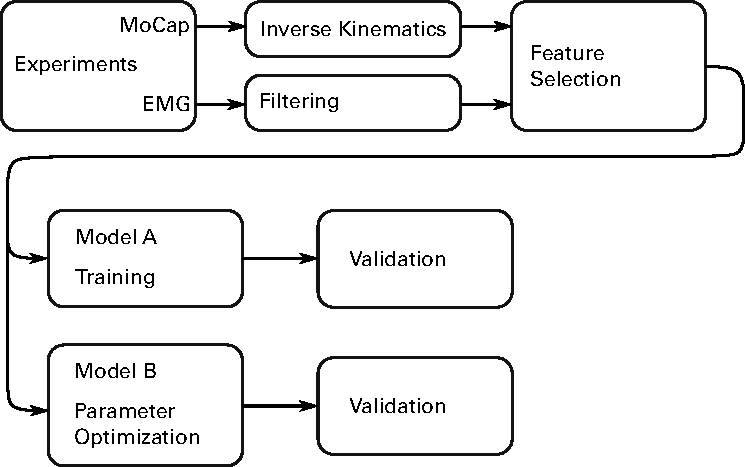
\includegraphics[width=0.8\textwidth]{images/summer_school_study/schematitc.pdf}%
  \caption{Upper Arm Movement Modeling:\\ Schematic workflow of data processing. In experiments, Motion Capture (MoCap) data and EMG signals were recorded. They were processed using inverse kinematics and filtering techniques, respectively. The size of the large datasets was reduced by selecting specific features. Those were used as training inputs for the two models A and B. The trained models were validated using a validation dataset that also originated from experiments.}%
  \label{fig:schematitc}%
\end{figure}%
%
I contributed mainly to the fields of data processing, especially filtering of EMG signals and feature selection, derivation and training of both models, A and B, their validation and the overall programming and visualization of the results. The respective fields are presented more detailed in the following, corresponding sections.

\subsection{Structure of this Chapter}
\Cref{sec:exp_study} gives an overview of the experiments, data processing and feature selection, which resulted in the required datasets. In \cref{sec:study_models}, the two models, A and B, are described. Results including the validation of the models and a discussion are given in \cref{sec:evaluation}. Conclusions follow in \cref{sec:study_conclusion}.

\section{Experimental Study}\label{sec:exp_study}

\begin{figure}%
    \centering%
    \def\svgwidth{5cm}%
    \input{images/summer_school_study/summer_school_study.pdf_tex}%
    \caption{Upper Arm Movement Modeling: \\Experimental setup for the triceps trials. The subject pulls down a rope over a pulley which is connected to a weight with mass $m_w$.
    Angles required for the kinematic formulation are the elbow angle, $\phi_e$, the forearm angle, $\phi_a$, and the angle of the weight, $\phi_w$. The length of the ulna bone is denoted by $\ell_u$.}%
    \label{fig:summer_school_study}%
\end{figure}%

Experiments are required to identify the model parameters for the particular subject. First, the experimental setup is described, then, details on the processing of the measured values are given. Then, the selection of feature points from the experimental data is described.

\subsection{Experimental Trials}

In a series of experiments, eight different actions of flexing and extending the elbow were performed by the subject. Weights of 3 kg and 5 kg were held in the hand during the elbow flexion trials. For the elbow extension trials, a pulley system was installed that redirected the force of the weight such that the downward movement of the forearm acted against the direction of the force. This is shown in \cref{fig:summer_school_study}. A detailed description of the experimental trials can be found in \cite{summerschool2019}.

Time series of position and velocity of the upper arm and the forearm were recorded using a Motion Capture system. It consisted of eight cameras that tracked three markers placed on shoulder, elbow and wrist of the subject. 

The elbow torque $\tau$ was computed as
\begin{equation*}
  \begin{array}{lll}
    \tau = m_w\,g\,\ell_u\,\sin(\phi_w) - m_{a}\,g\,\dfrac{\ell_u}{2}\,\sin(\phi_a),
  \end{array}
\end{equation*}
where $(m_w\,g)$ is the force of the weight, $m_{a}$ is the mass of forearm and hand, $\ell_u$ is the length of the ulna bone and $\phi_a$ and $\phi_w$ are the angles of the forearm and rope, as visualized in \cref{fig:summer_school_study}.

\subsection{Data Processing}
From the captured data, derived quantities of biceps ($B$) and triceps ($T$) muscles were estimated using a geometric model of the upper arm. 
The geometric model is available in the software OpenSim \cite{OpenSim2007} and was customized for the particular subject. The inverse kinematics module of OpenSim was used to estimate the muscle tendon unit lengths, $\ell_{\text{MTU},M}$, contraction velocities, $v_M=\dot{\ell}_M$, and moment arms, $r_{M}$, of the two muscles, $M\in\{B,T\}$.

EMG signals were captured by two electrodes on the skin at the biceps and triceps muscles. For both signals, several preprocessing steps were applied to obtain the inputs for the two models, A and B.

The raw signal was filtered with the same procedure as in \cite{Falisse2016}. First, a fourth-order Butterworth high pass filter with cutoff frequency 30 Hz was applied to reduce non-zero average voltages. Second, the resulting signal was full-wave rectified by taking the absolute value of every measured data point. Third, application of a fourth-order Butterworth low pass filter with 10 Hz cutoff frequency yielded a smoothed signal.
Forth, the resulting filtered EMG signals were normalized to the interval $[0,1]$, such that the value of 1 corresponds to the experimentally determined value of maximum voluntary contraction.

The measured EMG signals on the skin directly correspond to the electric excitation level $u$ in the muscle. Excitation leads to the release of free calcium ions within the sarcomere. Binding of calcium ions to myosin increases the concentration of cross-bridges. This concentration is commonly known as the muscular activation $\alpha$. The muscular activation directly corresponds to the produced force of the muscle \cite{Bayer2017}.

The concentration of free calcium ions is denoted as $\gamma$ and can be computed from the excitation $u$ by the following first order differential equation \cite{Hatze1977}
%
\begin{equation*}
  \begin{array}{lll}
    \dot{\gamma} = m\,(u - \gamma).
  \end{array}
\end{equation*}
%
We used the filtered EMG signal $u$ to obtain values for $\gamma$. \Cref{fig:emg_filtering} shows the raw and filtered EMG signals and the resulting free calcium concentration for a sample of the experimental data.

\begin{figure}%
  \centering%
  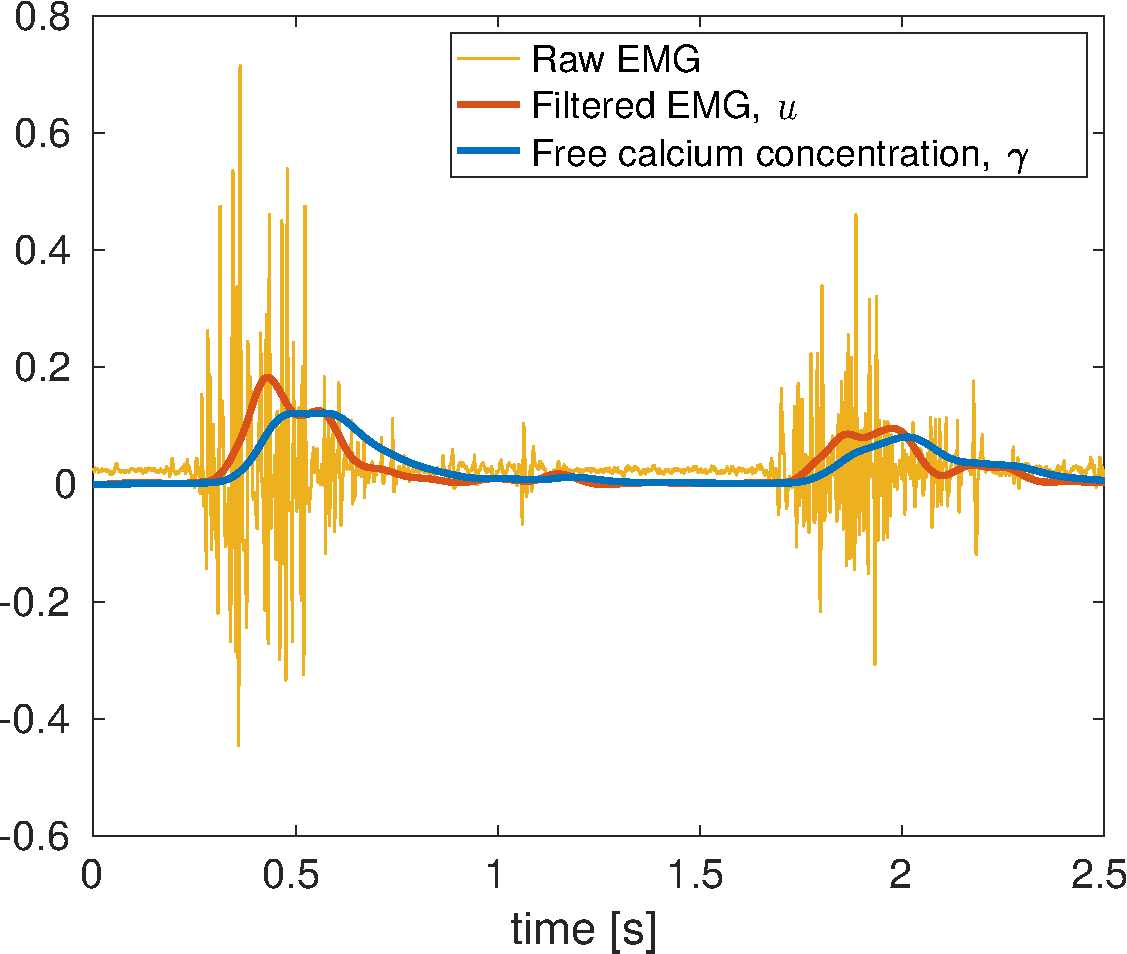
\includegraphics[width=0.8\textwidth]{images/summer_school_study/emg_filtering.pdf}%
  \caption{From raw EMG data of the biceps (yellow) to the filtered signal $u$ (red) and the free calcium concentration $\gamma$ (blue). The data are taken from the beginning of the first elbow flexion experiment. It can be seen that the filtering smooths out the initial signal and removes the constant offset. The free calcium ion concentration follows the filtered EMG with a short delay.}%
  \label{fig:emg_filtering}%
\end{figure}%

The activation of the muscle $\alpha$ does not only depend on the free ion concentration $\gamma$ but also on the current state of muscle contraction. This excitation-contraction coupling has to be described by a dynamic system of ODEs and is included in model B.
Therefore, preprocessing is completed with computing the free calcium concentration $\gamma$ and not the activation $\alpha$.

\subsection{Feature Selection} \label{sec:study_feature_selection}

The eight experimental trials were split into $n_\text{trials}=7$ experiments to be used for model identification and one for validation.
The total number $N$ of captured values in the training experiments was large, such that not all points could be used for training of models A and B.
To reduce the amount of data and, thus, speed up the computation, we selected $n \ll N$ featured values with the assumption that they are representative for the whole data set.
For every experimental trial, we choose the same fixed number $n_\text{per\_trial}$ of data points.
Our selection algorithm identifies $n_\text{per\_trial}$ timesteps, $t_i, i=1, \dots, n$ such that the summed values of the free calcium concentrations $\gamma_B(t_i) + \gamma_T(t_i)$ for biceps and triceps are evenly distributed along the value range.
This leads to $n = n_\text{trials} \cdot n_\text{per\_trial}$ selected data points.

The set of training data $\mathcal{D} = \mathcal{X} \times \mathcal{Y}$ consists of the $n$ selected vectors of the experimental values that are the input to the system of muscles, $\bfx_i \in \mathcal{X}, i=1,\dots, n$, together with the observed output values, $y_i \in \mathcal{Y}, i=1,\dots,n$.
The input vectors contain values for muscle tendon unit lengths, contraction velocities, moment arms and free calcium ion concentrations for biceps and triceps each, $\bfx_i = (\ell_{\text{MTU},B}, \ell_{\text{MTU},T}, v_B, v_T, r_{B}, r_{T}, \gamma_B, \gamma_T)^\top(t_i)$. The output values consist of the elbow torques, $y_i = \tau(t_i)$. This data set, $\mathcal{D}$, serves as training input for both models, A and B.

\section{Models}\label{sec:study_models}

The current section describes the two model approaches that can predict elbow torques from experimental input data. \Cref{sec:data_driven_model} introduces the non-parametric, data driven model A. \Cref{sec:biophysical_model} presents the biophysically based model B. It requires a parameter optimization, which is described in \cref{sec:parameter_optimization}.

\subsection{Data-driven Model A}\label{sec:data_driven_model}

The first modeling approach uses a non-parametric model. Such a model approximates the function $f$ that maps from input to output data points. The function $f$ is learned from the training data set. Regression is used to obtain predictions for new data points. In our case, we use a stochastic model that considers the probability distribution of the model function.

We use the method of \emph{Gaussian Process Regression}. A Gaussian process is a collection of random variables such that the joint distribution of every finite subset of these random variables is multivariate normal (Gaussian).
In our example, each input data point in the space of measured values, $\bfx \in \mathcal{X}$ has an associated random variable $f(\bfx)$ that describes the output of the model for this point.

A Gaussian process, $\mathcal{GP}$, is characterized by a mean function $m(\bfx)$ and a kernel function $k(\bfx,\bfx')$ that models the covariance between any pair $(\bfx, \bfx') \in \mathcal{X} \times \mathcal{X}$ of points. Different choices of kernel functions are possible and can depend on hyperparameters $\bfpsi$. Describing observed values $y$ by a Gaussian process distribution can be expressed as
\begin{equation*}
  \begin{array}{lll}
    f(x) \approx y \sim \mathcal{GP}\big(m(\bfx), k(\bfx,\bfx',\bfpsi)\big).
  \end{array}
\end{equation*}
This representation is non-parametric in the sense that no particular parametric form of the function $y=f(\bfx)$ is assumed whose (biophysical) parameters would be determined. Instead, a generic probabilistic model is constructed using the observed function values at measured inputs $\bfx_i \in \mathcal{X}$.
%More specifically, the conditional distribution $p(y|\bfx)$ considered.

Gaussian Process Regression is based on \emph{Bayesian Inference} to update a prior belief of the model to a posterior model using information contained in observations of the process.
The observed data are the set of measurements $\mathcal{D}$. 

The \emph{prior} distribution $p(\bff\mid\mathcal{X},\bfpsi)$ for the vector of function values $\bff$ is described by the Gaussian process,
\begin{equation*}
  \begin{array}{lll}
    p(\bff\mid\mathcal{X},\bfpsi) = \mathcal{N}(\bff\mid\bfm,\bfK),
  \end{array}
\end{equation*}
with mean values $\bfm = (m(\bfx_i))^\top_{i=1,\dots,n}$ and covariance matrix $\bfK$ with $K_{ij} = k(\bfx_i,\bfx_j,\bfpsi).$

The \emph{likelihood} $p(\bfy\mid f(\bfx), \bftheta)$ describes the probability of an observation $\bfy$ given a particular model $f$. The vector $\bftheta$ denotes additional parameters of the likelihood. 

Using Bayes' rule, the \emph{posterior} distribution $p(\bff\mid\mathcal{D})$ of the function values $\bff$ can be computed from prior and likelihood as
\begin{equation*}
  \begin{array}{lll}
    p(\bff\mid\mathcal{D},\bftheta,\bfpsi) 
      = \dfrac{p(\bfy\mid\bff,\bftheta)\,p(\bff\mid\mathcal{X},\bfpsi)}{p(\mathcal{D}\mid\bftheta,\bfpsi)}.
  \end{array}
\end{equation*}
This results in a measure for the uncertainty of the model $f$ at unobserved points $\bfx_\ast \notin \mathcal{D}$. 

Additionally, the fact that the measured quantities in the experiments are subject to measurement noise can be incorporated into the model.
The assumption 
\begin{equation*}
  \begin{array}{lll}
    y = f(\bfx) + \eps
  \end{array}
\end{equation*}
adds a normally distributed random variable of observational noise $\eps \sim \mathcal{N}(0,\sigma_n^2)$ to the formulation. The noise variance $\theta = \sigma_n^2$ is an additional parameter of the likelihood. 
It is also possible to explicitly model the mean function $m(\bfx)$. By replacing the model $f(\bfx)$ by $g(\bfx) = f(\bfx) + \bfh(\bfx)^\top \bfbeta$, i.e.
\begin{align*}
  %\begin{array}{rlrl}
    y &= f(\bfx) + \bfh(\bfx)^\top \bfbeta + \eps, \quad 
    &\text{ with } f(x) &\sim\mathcal{GP} \big(m(\bfx), k(\bfx,\bfx',\bfpsi)\big),\\[4mm]
    && \eps &\sim \mathcal{N}(0,\sigma_n^2),
  %\end{array}
\end{align*}
we allow for a global trend in the data that is formulated in terms of a vector of explicit basis functions $\bfh(\bfx)$ and corresponding coefficients $\bfbeta$.

The algorithm for Gaussian Process Regression involves estimating the following values from the given data during the training phase. The hyperparameters of the covariance function $\bfpsi$, the noise variance $\bftheta$, and the coefficients of the fixed basis functions $\bfbeta$ are determined by solving an optimization problem. The computation involves matrix inversions and has a computational complexity $\O(n^3)$, i.e. is cubic in the number of data points. For details, the reader is referred to the literature \cite{Rasmussen2005,kuss2006gaussian}.

In our study, training of the Gaussian Process of model A was performed using the ready to use implementation provided by MATLAB.
We parametrized the covariance by a squared exponential kernel and used constant basis functions, $\bfh(x) = 1$. We enabled observational noise, its variance $\bftheta = \sigma_n^2$ was found by optimization during training of the model.

%$p(\bff^\ast | \mathcal{D},\mathcal{X}^\ast)$
\subsection{Biophysical Model B}\label{sec:biophysical_model}

Extension of the elbow is governed by the triceps brachii muscle.
During elbow flexion, three muscles are involved: biceps brachii, brachialis and brachioradialis. For simplicity, only biceps brachii, which contributes most of the moment, is explicitly considered in the current study. The effects of the other two muscle are contained in the biceps brachii model in a lumped manner.

Thus, the biophysical model consists of two Hill-type muscle models, for biceps and triceps, respectively. The muscle models are arranged around a hinge joint for the elbow angle. The muscle forces contribute to the torque at the elbow over their respective moment arms.

Hill-type models describe the macroscopic, dynamic mechanical behavior of an entire muscle along a one-dimensional line of action.
The behavior is formulated by phenomenological, mathematical functions that have to be parametrized to fit experimental observations.

%Such models are often used to compute muscle forces in simulations of various movements, e.g. \cite{Siebert2003}, \cite{Kistemaker2006}.
Multiple variants of Hill-type models exist that use various configurations of mechanical elements to consider different properties and functionalities of the muscle. The original model was proposed in \cite{Hill1938}. It contains a contractile element (CE) and two elastic elements, arranged in series and in parallel to the CE.
The authors of \cite{Siebert2008} compare two different approaches using these three elements. The effect of tension in eccentric contractions is added to the Hill-type model by \cite{Till2008}. The authors of \cite{Gunther2007} add a forth, damping element to account for high-frequency damping of the muscle tissue. In \cite{Morl2012}, electromechanical delay is investigated with and without the additional damping element. 

\begin{figure}%
  \centering%
  \def\svgwidth{0.5\textwidth}
  \input{images/summer_school_study/hilltype.pdf_tex}%
  \caption{Mechanical structure of the Hill-type muscle model. The force generating contractile element (CE) is parallel-connected to the parallel elastic element (PEE) and connected in series to a second parallel-connected structure consisting of the serial elastic element (SEE) and the serial damping element (SDE). The length $l_\text{MTU}$ of the whole muscle tendon unit is composed of the common length $l_\text{CE}$ of CE and PEE and the common length $l_\text{SEE}$ of SEE and SDE. The variable $l_\text{CE}$ is an internal state of the model.}
  \label{fig:hilltype}%
\end{figure}%

\newcommand{\CE}{\text{CE}}
\newcommand{\MTU}{\text{MTU}}

We employ the four-element Hill-type muscle model that is described by \cite{Hilltype2014}. Its structure is visualized in \cref{fig:hilltype}. It consists of four components: the contractile element (CE), the parallel elastic element (PEE), the serial elastic element (SEE), and the serial damping element (SDE). Inputs to the model are the muscular activation $\alpha(t)$, the length $l_\MTU(t)$ and the contraction velocity $\dot{l}_\MTU(t)$ of the muscle tendon unit (MTU).
The output of the model is the muscle force $f_\text{MTU}(t)$. The model contains one internal state variable, the length $l_\text{CE}(t)$ of the CE. The muscle dynamics determine this internal length and its time derivative, the contraction velocity $\dot{l}_\text{CE}(t)$ of the CE.

The resulting force of the MTU is given as sum of the forces of the respective parallel elements as visualized in \cref{fig:hilltype}:
\begin{equation}\label{eq:hill_type0}
  \begin{array}{lll}
    F_\MTU = F_\CE(l_\CE, \dot{l}_\CE, \alpha) + F_\text{PEE}(l_\CE) = F_\text{SEE}(l_\CE,l_\MTU) + F_\text{SDE}(l_\CE,\dot{l}_\CE,\dot{l}_\MTU,\alpha).
  \end{array}
\end{equation}
The force terms of the four elements, $F_\CE, F_\text{PEE}, F_\text{SEE}$ and $F_\text{SDE}$ are described by analytical functions that use a total of 19 parameters. A description of the detailed equations and parameters can be found in \cite{Hilltype2014}. In the following, an overview over the formulation is given with a focus on the piecewise formulated terms that contribute to the overall muscle model. In the following formulations, underlined variables designate constant parameters that either have to be specified or follow from other given parameters.

The muscle output force $F_\text{MTU}$ is computed by the second identity of \cref{eq:hill_type0}, i.e., from the forces $F_\text{SEE}$ and $F_\text{SDE}$. The force $F_\text{SEE}$ acting in the SEE is formulated as a continuous piecewise function with a constant zero, an exponential and a linear branch:
\begin{equation*}
  \begin{array}{lll}
    F_\text{SEE}(\ell_\CE,\ell_\MTU) = \begin{cases}
      0, & \ell_\text{SEE} < \underline{l_{\text{SEE},0}}\\[2mm]
      \underline{K_\text{SEE,nl}}(\ell_\text{SEE} - \underline{\ell_\text{SEE,0}})^{\underline{\nu_\text{SEE}}}, & \ell_\text{SEE} < \underline{\ell_\text{SEE,nll}}\\[2mm]
    \underline{\Delta F_\text{SEE,0}} + \underline{K_\text{SEE,l}}(\ell_\text{SEE} - \underline{\ell_\text{SEE,nll}}), & 
    \ell_\text{SEE} \geq \underline{\ell_\text{SEE,nll}}
    \end{cases}, \quad \text{with } \ell_\text{SEE} = \ell_\MTU - \ell_\CE.
  \end{array}
\end{equation*}

The damping force $F_\text{SDE}$ in the SDE is proportional to the lengthening velocity ${\dot{\ell}_\text{SEE} = \dot{\ell}_\MTU - \dot{\ell}_\CE}$ of this element. It is given by
\begin{equation}\label{eq:sde_force}
  \begin{array}{lll}
    F_\text{SDE}(l_\CE,\dot{l}_\CE,\dot{l}_\MTU,\alpha) \\ \qquad = \underline{D_\text{SDE,max}}\left( (1-\underline{R_\text{SDE}}) \dfrac{F_\text{PEE}(\ell_\CE)+F_\text{CE}(\ell_\CE, \dot{\ell}_\CE, \alpha)}{\underline{F_\text{max}} + \underline{R_\text{SDE}}} \right) (\dot{\ell}_\MTU - \dot{\ell}_\CE).
  \end{array}
\end{equation}
The amount of damping is dependent on the force $F_\MTU$ of the MTU which appears in the nominator of the fraction in \cref{eq:sde_force} as the sum of the forces $F_\text{PEE}$ and $F_\CE$. Formulas for these two forces are given in the following.

The force $F_\text{PEE}$ of the PEE is formulated piecewise as a shifted and cut off polynomial function:
\begin{equation}\label{eq:fpee}
  \begin{array}{lll}
    F_\text{PEE}(\ell_\CE) = \begin{cases}
      0, & \ell_\CE < \underline{\ell_{\text{PEE},0}}\\[4mm]
    \underline{K_\text{PEE}}(l_\CE - \underline{l_{\text{PEE},0}})^{\underline{\nu_\text{PEE}}},& \ell_\CE \geq \underline{\ell_{\text{PEE},0}}
    \end{cases}.
  \end{array}
\end{equation}

The force $F_\CE$ of the CE is the active force produced by the muscle and is given by:
\begin{equation}\label{eq:fce}
  \begin{array}{lll}
    F_\CE(l_\CE, \dot{l}_\CE, \alpha) 
    = \underline{F_\text{max}} \left(
    \dfrac{\alpha\,F_\text{isom}(\ell_\CE) + A_\text{rel}(\dot{\ell}_\CE,\ell_\CE,\alpha)}
    {1 - 
    \frac{\dot{\ell}_\CE}
    {B_\text{rel}(\dot{\ell}_\CE,\ell_\CE,\alpha)\,\ell_{\CE,\text{opt}}}}\right)
    - A_\text{rel}(\dot{\ell}_\CE,\ell_\CE,\alpha).
  \end{array}
\end{equation}
It can be seen that the active force depends on the activation level $\alpha$. 
The formulation of $F_\CE$ contains the two main characteristic curves for muscle forces, the force-length relation and the force-velocity relation.

The force-length relation is modeled by the function $F_\text{isom}(\ell_\CE)$ of isometric force, which describes the relative force for the condition $\dot{\ell}_\CE = 0$. This function is formulated piecewise for CE lengths $\ell_\CE$ smaller and larger than an optimal length $\ell_\text{CE,opt}$. 

The force-velocity relation follows from the auxiliary functions $A_\text{rel}(\dot{\ell}_\CE,\ell_\CE,\alpha)$ and $B_\text{rel}(\dot{\ell}_\CE,\ell_\CE,\alpha)$. These functions have different forms for concentric ($\dot{\ell}_\CE < 0$) and eccentric ($\dot{\ell}_\CE \geq 0$) conditions as well as for the two ranges of CE  length, $\ell_\CE < \ell_\text{CE,opt}$ and $\ell_\CE \geq \ell_\text{CE,opt}$.

\begin{figure}%
  \centering%
  \begin{subfigure}[t]{0.9\textwidth}%
    \centering%
    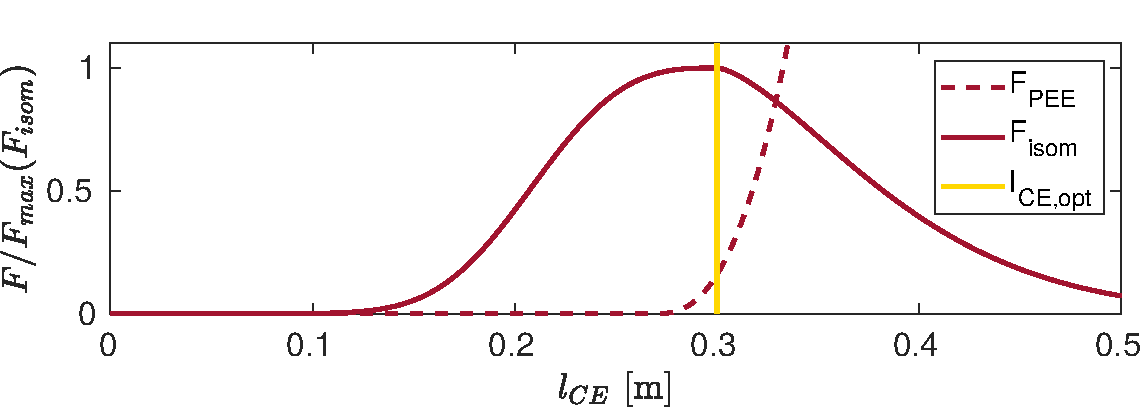
\includegraphics[width=\textwidth]{images/summer_school_study/force_curves_generic_length.pdf}%
    \caption{Force-length curves of the PEE (dashed red line) and isometric force $F_\text{isom}$ (solid red line) for an isometric condition ($\dot{l}_\CE=0$), normalized to the maximum isometric force. The optimal length $l_\text{CE,opt}$ of the CE is shown as yellow vertical line. The force $F_\text{PEE}(l_\CE)$ of the PEE is zero for $l_\CE < 0.9\,l_\text{CE,opt}$. The isometric contraction force $F_\text{isom}$ is formulated piecewise by two branches separated by $l_\text{CE,opt}$.}%
    \label{fig:force_curves_generic_length}%
  \end{subfigure}\\[6mm]
  \begin{subfigure}[t]{0.9\textwidth}%
    \centering%
    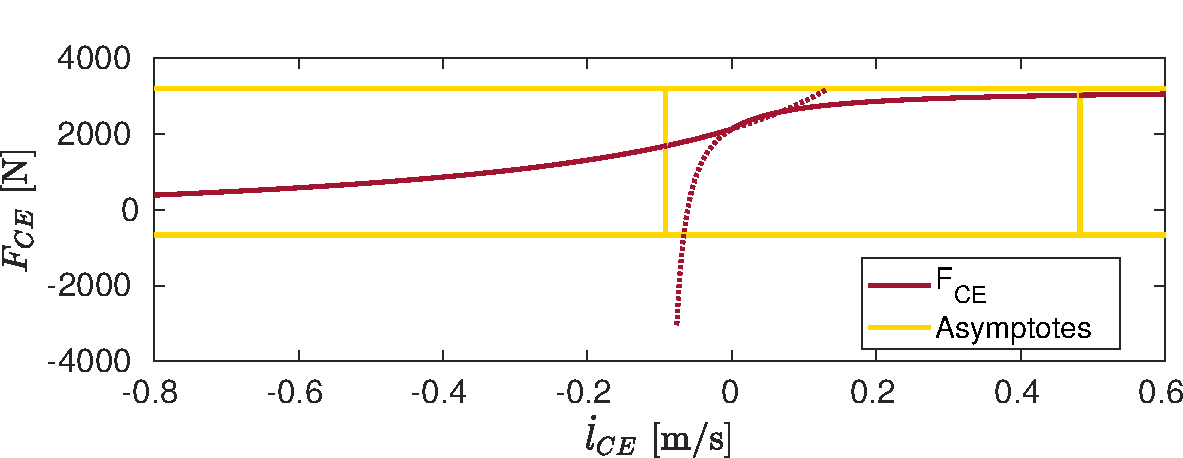
\includegraphics[width=\textwidth]{images/summer_school_study/force_curves_generic_velocity.pdf}%
    \caption{Force-velocity curve $F_\CE(\dot{l}_\CE)$ of the CE at optimal length $l_\CE=l_{\CE,\text{opt}}$, and for activation level $\alpha=0.5$. The function (red solid line) is formulated piecewise, graphs of the base functions of the two branches continue as red dotted lines. Their limits and singularities are visualized by the yellow horizontal and vertical asymptotes.}%
    \label{fig:force_curves_generic_velocity}%
  \end{subfigure}%
  \caption{Force-length and force-velocity relations for the muscle model with generic parameters taken from literature \cite{Hilltype2014}.}%
  \label{fig:force_curves_generic}%
\end{figure}%

\Cref{fig:force_curves_generic} visualizes the two main characteristic curves of the model. 
\Cref{fig:force_curves_generic_length} shows how the generated force depends on the length of the CE. 
The active force $F_\CE$, given by \cref{eq:fce}, is visualized by the solid red line. It has its maximum at the optimal length $l_\text{CE,opt}$ of the CE. This can be explained by the overlap of actin and myosin filaments in the sarcomere. The overlap is lower when the actin filaments are pulled apart or pushed together. A higher overlap leads to a higher force output.

The dashed line in \cref{fig:force_curves_generic_length} represents the passive force $F_\text{PEE}$ of the elastic muscular tissue, formulated in \cref{eq:fpee}. The passive force is essentially generated by the titin proteins in the sarcomere. Only starting from a certain length, the structure exerts reaction forces against lengthening forces to avoid overstretching of the muscle.

\cref{fig:force_curves_generic_velocity} shows the force-velocity relation of the Hill-type model. The curve of $F_\CE(\dot{l}_\CE)$ is composed of two branches: 
The concentric branch for shortening contraction with $\dot{l}_\CE \leq 0$ and the eccentric branch for lengthening contraction with $\dot{l}_\CE > 0$. It can be seen that the generated force increases monotonically over the lengthening velocity. It approaches a limit for maximum positive and negative velocity. These limits can be adjusted by parameters of the model and are exemplary for how the shape of the curves of a Hill-type model can be parametrized.

In addition to the resulting muscle force $F_\MTU$, a formulation for the internal state variable $\ell_\CE$ is required.
The second identity of \eqref{eq:hill_type0} can be solved for the lengthening velocity $\dot{\ell}_\CE$ of the CE to get an evolution equation for the length $\ell_\CE$ of the CE. The derivation and the resulting formula can be found in \cite{Hilltype2014}.

To describe the activation dynamics, i.e., the evolution of the muscle activation ${\alpha \in [0,1]}$, the model of Hatze et al. \cite{Hatze1977} is used.
The activation is computed depending on the free calcium ion concentration $\gamma$ and the length $\ell_\CE$ of the CE by
\begin{equation*}
  \begin{array}{lll}
    \alpha(\ell_\CE,\gamma) = \dfrac{\underline{a_0} + \big(\rho(\ell_\CE)\,\gamma\big)^3}
    {1 + \big(\rho(\ell_\CE)\,\gamma\big)^3}.
  \end{array}
\end{equation*}
The function $\rho$ is given by
\begin{equation*}
  \begin{array}{lll}
    \rho(\ell_\CE) = \underline{c}\,\underline{\eta}\,\dfrac{(\underline{k}-1)\,\ell_\CE}{(\underline{k} - \ell_\CE/\ell_\text{CE,opt})\,l_\text{CE,opt}}.
  \end{array}
\end{equation*}
All used parameter values for the activation dynamics can be found in \cite{Bayer2017}.

In summary, we get the following coupled system of differential-algebraic equations, where $f_\CE$ and $f_\alpha$ denote the respective formulas:
\begin{align}
  F_\MTU &= F_\MTU(\ell_\MTU,l_\CE,\dot{l}_\CE,\alpha),      \label{eq:hill_type1} \\[4mm]
  \dot{l}_\CE &= f_\CE(l_\CE,\ell_\MTU,\dot{l}_\MTU,\alpha), \label{eq:hill_type2}\\[4mm]
  \alpha &= f_\alpha(\gamma, l_\CE).                      \label{eq:hill_type3}
\end{align}

To compute the joint torque in a system of an agonist and antagonist muscle pair, two instances of the presented Hill-type muscle model can be used. In our study considering the upper arm, the torque $\tau$ at the elbow is computed by multiplying the predicted forces $F_{\MTU,B}$ and $F_{\MTU,T}$ of biceps and triceps with the corresponding moment arms $\hat{r}_B$ and $\hat{r}_T$:
\begin{equation}\label{eq:muscle_torque}
  \begin{array}{lll}
    \tau = F_{\MTU,B}(l_{\MTU,B},\dot{l}_{\MTU,B},\alpha_B) \cdot \hat{r}_B - F_{\MTU,T}(l_{\MTU,T},\dot{l}_{\MTU,T},\alpha_T) \cdot \hat{r}_T.
  \end{array}
\end{equation}

\subsection{Parameter Identification for Model B}\label{sec:parameter_optimization}
%
The process of model identification finds the parameters that make the model B predict correct values for the specific subject, i.e., minimizes the error in the predicted outcome for the training data set.

The following minimization is performed:
\begin{align}
  &&\min\limits_{\substack{\bftheta_M,l_{\CE,M}(t), \\\forall M \in \{B,T\}, \,\forall t \in \mathcal{T}}} &\sum\limits_{t\in \mathcal{T}}|\tau(t) - \hat{\tau}(t)|^2
   \label{eq:opt_1}\\[4mm]
  &&\text{s.t. }\forall t \in \mathcal{T}:\quad &\tau(t) = F_{\MTU,B}(t,l_{\CE,B},\bftheta_B) \cdot \hat{r}_B(t) \notag\\
      &&&\qquad\quad- F_{\MTU,T}(t,l_{\CE,T},\bftheta_T) \cdot \hat{r}_T(t),                 \label{eq:opt_2}\\[4mm]
  &&& \dot{l}_{\CE,M}(t) = \dot{\hat{l}}_{\MTU,M}(t),\quad M \in \{B,T\},      \label{eq:opt_3}\\[4mm]
  &&& \bftheta_B, \bftheta_T \in \Theta,                                       \label{eq:opt_4}\\[4mm]
  &&& l_{\CE,M}(t) \in [0,l_{\MTU,M}(t)],\quad M \in \{B,T\}.                  \label{eq:opt_5}
\end{align}

The optimization variables are the parameters $\bftheta_B$ and $\bftheta_T$ for the biceps and triceps Hill-type models and the lengths $l_{\CE,B}(t)$ and $l_{\CE,T}(t)$ of the contractile elements for both models at every point in time. The variables designated as $\hat{\square}$ are the measured quantities from the training experiments. The objective function given in \cref{eq:opt_1} penalizes the difference between computed torque $\tau$ and measured torque $\hat{\tau}$ at every timestep $t \in \mathcal{T}$ of the training data. 

\Cref{eq:opt_2} computes the torque values and follows from \cref{eq:muscle_torque} of the muscle model. For every point in time, the predicted forces $F_{\MTU,B}$ and $F_{\MTU,T}$ are multiplied with the measured moment arms $\hat{r}_B$ and $\hat{r}_T$.

In \cref{eq:opt_3}, the contraction velocities are constrained to the measured values. Because the lengthening velocity $\dot{l}_\CE$ of the CE is an internal quantity and, thus, cannot be observed in experiments, we assume it to be equal to the lengthening velocity of the whole muscle: $\dot{l}_\CE \approx \dot{l}_{\MTU} = \dot{l}_\text{CE} + \dot{l}_\text{SEE}$. This requires the assumption $\dot{l}_{\text{SEE}} \approx 0$ which can be justified given the low dynamic nature of the experiments.

By \cref{eq:opt_4}, we bound each of the parameters $\bftheta_B$ and $\bftheta_T$ to a range between half and twice the generic value from literature.
The lengths of the CEs are constrained by \cref{eq:opt_5} to be positive and smaller than the length of the MTU.

All optimization variables are normalized to improve the numerical conditioning of the optimization problem. 
The parameters $\bftheta_B$ and $\bftheta_T$ are normalized with respect to generic values from literature that were taken from \cite{Gunther2007, Morl2012, Hilltype2014}. The initial values are set to one, which corresponds to the generic literature values.
The internal states $l_{\CE,B}$ and $l_{\CE,T}$, are normalized with respect to the measured MTU lengths $\hat{l}_{\MTU,B}$ and $\hat{l}_{\MTU,T}$ and initialized with zero.

%For training of model B, the optimization problem for the parameters needed to be solved. 
We implemented the Hill-type models and the constraints in MATLAB and used the nonlinear programming implementation, \code{fmincon}, to minimize the given bounded and nonlinear constrained, multivariable function.
In our study, the total number of optimization variables is computed by $2\cdot 19 + 2n = 598$, as each of the parameter vectors $\bftheta_B,\bftheta_T$ had 19 entries. 

\section{Results and Discussion}\label{sec:evaluation}

In the following, results of connecting the two model formulations, A and B, to the experimental data are presented.
At first, \cref{sec:res_feature_selection} gives details on the preprocessed data. The training phase is described in \cref{sec:res_training}. Applying the trained models to the validation data is done in \cref{sec:res_validation}. Then, \cref{sec:res_simplified_a} tests a simplified version for model A. Then, \cref{ref:res_insights_b} shows some insights into the optimized parameter values for model B.

\subsection{Feature Selection}\label{sec:res_feature_selection}
% intro
The experimental data is split into a training and a validation dataset. \Cref{fig:selected_points} shows the processed data of the training data set. In total, we captured $N=\num{34934}$ data points for the seven experimental trials. Out of these, we select $n_\text{per\_trial}=\num{40}$ feature points in every trial, leading to a total of $n=n_\text{per\_trial}\cdot n_\text{trials}=\num{280}$ points. The selected points are visualized by crosses in the top plot of \cref{fig:selected_points}. It can be seen that the algorithm described in \cref{sec:study_feature_selection} distributes the feature points equally along the $\gamma$ axis.

\begin{figure}%
  \centering%
  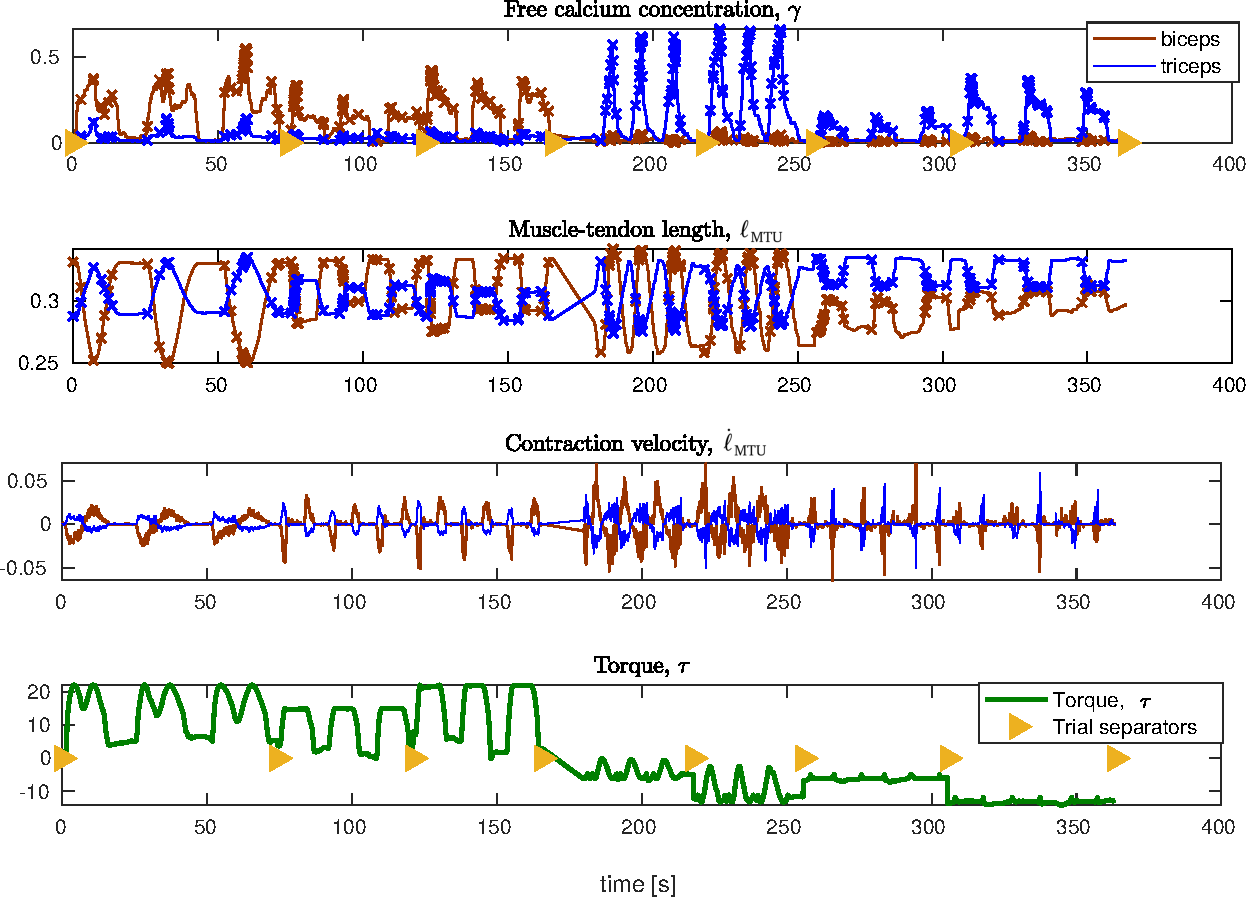
\includegraphics[width=\textwidth]{images/summer_school_study/selected_points.pdf}%
  \caption{Processed experimental values over time that were used for training of both models. The concatenated data of seven trials are shown, which yield an end time of $\SI{363.32}{s}$. The individual trials are separated by the yellow triangles on the $x$-axis. The three upper plots show the values of $\gamma, \ell_\MTU$ and $\dot{l}_\MTU$ for both biceps (brown) and triceps (blue), the bottom plot shows the elbow torque $\tau$. The selected feature points are visualized as crosses in the two top plots. In the upper-most plot, it can be seen that the first three trials, which correspond to elbow flexion, mainly activated the biceps muscle, whereas in the last four trials, corresponding to elbow extension, the triceps is more active.
}%
  \label{fig:selected_points}%
\end{figure}%

\subsection{Training of the Models}\label{sec:res_training}
%
Training of model A consists of estimating the hyperparameters for the Gaussian Process Regression model from the training data.

For model B, the optimization problem for the biophysical parameters is solved. The resulting parameter values and their relation to the initial values are summarized in \cref{tab:model_b_parameters}. It can be seen that none of the final parameter values is limited by the constraints, which would be $\SI{-50}{\percent}$ and +\SI{100}\percent. However, it was observed that including the constraints helps the optimizer to stay in the valid range of meaningful model parameters and, thus, reach the optimum faster.

\begin{table}[t] 
  \centering
  %\begin{scriptsize}
  
    \begin{tabular}{@{}llllll@{}}
%\hline
 %| param              | biceps   |            | triceps  |            %|
 %| ------------------ | -------- | ---------- | -------- | ---------- %|
 %| CE_F_max           | +11.03 % | 4729.97    | -49.04 % | 2171.04    |
 %| CE_l_CEopt         | +31.72 % | 0.40       | -25.36 % | 0.22       |
 %| CE_DeltaW_limb_des | +10.86 % | 0.39       | +10.86 % | 0.39       |
 %| CE_DeltaW_limb_asc | +91.61 % | 0.67       | +5.05 %  | 0.37       |
 %| CE_v_CElimb_des    | +10.86 % | 1.66       | +10.86 % | 1.66       %|
 %| CE_v_CElimb_asc    | -46.39 % | 1.61       | +95.87 % | 5.88       |
 %| CE_A_rel0          | +14.03 % | 0.29       | -20.34 % | 0.20       |
 %| CE_B_rel0          | +77.51 % | 3.99       | +41.38 % | 3.18       |
 %| CE_S_eccentric     | -4.12 %  | 1.92       | +22.92 % | 2.46       |
 %| CE_F_eccentric     | -30.94 % | 1.04       | +36.79 % | 2.05       |
 %| PEE_L_PEE0         | +10.86 % | 1.00       | +10.86 % | 1.00       |
 %| PEE_l_PEE0         | +10.86 % | 0.30       | +10.86 % | 0.30       |
 %| PEE_v_PEE          | +10.86 % | 2.77       | +10.86 % | 2.77       |
 %| PEE_F_PEE          | +10.86 % | 2.22       | +10.86 % | 2.22       |
 %| PEE_K_PEE          | +10.86 % | 1410470.38 | +10.86 % | 1410470.38 |
 %| SDE_D_SE           | +10.86 % | 0.33       | +10.86 % | 0.33       |
 %| SDE_R_SE           | +8.63 %  | 0.01       | -10.99 % | 0.01       |
 %| SDE_d_SEmax        | +8.41 %  | 513.16     | -10.64 % | 422.98     |
 %| SEE_l_SEE0         | -24.95 % | 0.13       | -10.28 % | 0.15       |
 %| SEE_DeltaU_SEEnll  | +59.16 % | 0.07       | +23.58 % | 0.05       |
 %| SEE_DeltaU_SEEl    | +63.34 % | 0.03       | +19.02 % | 0.02       |
 %| SEE_DeltaF_SEE0    | -42.40 % | 327.16     | +64.75 % | 935.78     |
 
% contractile element (CE)
%===========================
%  CE_F_max                         % F_max in [N] for Extensor (Kistemaker et al., 2006)
%  CE_l_CEopt                       % optimal length of CE in [m] for Extensor (Kistemaker et al., 2006)
%* CE_DeltaW_limb_des = 0.35;       % width of normalized bell curve in descending branch (Moerl et al., 2012)
%* CE_DeltaW_limb_asc = 0.35;       % width of normalized bell curve in ascending branch (Moerl et al., 2012)
%* CE_v_CElimb_des = 1.5;           % exponent for descending branch (Moerl et al., 2012)
%  CE_v_CElimb_asc = 3.0;           % exponent for ascending branch (Moerl et al., 2012)
%* CE_A_rel0 = 0.25;                % parameter for contraction dynamics: maximum value of A_rel (Guenther, 1997, S. 82)
%* CE_B_rel0 = 2.25;                % parameter for contraction dynmacis: maximum value of B_rel (Guenther, 1997, S. 82)
%  eccentric force-velocity relation:
%* CE_S_eccentric  = 2;             % relation between F(v) slopes at v_CE=0 (van Soest & Bobbert, 1993)
%  CE_F_eccentric  = 1.5;           % factor by which the force can exceed F_isom for large eccentric velocities (van Soest & Bobbert, 1993)

% paralel elastic element (PEE)
%===============================
%  PEE_L_PEE0   = 0.9;                               % rest length of PEE normalized to optimal lenght of CE (Guenther et al., 2007)
%  PEE_v_PEE    = 2.5;                               % exponent of F_PEE (Moerl et al., 2012)
%  PEE_F_PEE    = 2.0;                               % force of PEE if l_CE is stretched to deltaWlimb_des (Moerl et al., 2012)

% serial damping element (SDE)
%=============================
%* SDE_D_SE    = 0.3;               % xxx dimensionless factor to scale d_SEmax (Moerl et al., 2012)
%* SDE_R_SE    = 0.01;              % minimum value of d_SE normalised to d_SEmax (Moerl et al., 2012)
%  SDE_d_SEmax = SDE_D_SE*(CE_F_max*CE_A_rel0)/(CE_l_CEopt*CE_B_rel0);
                                    % maximum value in d_SE in [Ns/m] (Moerl et al., 2012)

% serial elastic element (SEE)
% ============================
%  SEE_l_SEE0        = 0.172;       % rest length of SEE in [m] (Kistemaker et al., 2006)
%  SEE_DeltaF_SEE0   = 568;         % both force at the transition and force increase in the linear part in [N] (~ 40% of the maximal isometric muscle force)
%  SEE_DeltaU_SEEnll = 0.0425;      % relativ stretch at non-linear linear transition (Moerl et al., 2012)
%* SEE_DeltaU_SEEl   = 0.017;       % relativ additional stretch in the linear part providing a force increase of deltaF_SEE0 (Moerl, 2012)
% 
     \toprule
    \textbf{CE} 
      & $F_{\mathrm{max}}\,[\mathrm{N}]$
      & $l_{\mathrm{CE},opt}\,[\mathrm{m}]$ 
      & $\Delta W_{d} \,[\;]$ 
      & $\Delta W_{a} \,[\;]$ 
      & $\nu_{\mathrm{CE},d} \,[\;]$ \\  \midrule
    Generic & $4260$ & $0.3$ & $0.35$ & $0.35$ & $1.5$  \\ %\hline
    Biceps  & $+\SI{11.0}{\percent}$ & $+\SI{31.7}{\percent}$ & $+\SI{10.9}{\percent}$ & $+\SI{91.6}{\percent}$ & $+\SI{10.9}{\percent}$  \\ %\hline
    Triceps & $-\SI{49.0}{\percent}$ & $-\SI{25.4}{\percent}$ & $+\SI{10.9}{\percent}$ & $+\SI{5.1}{\percent}$ & $+\SI{10.9}{\percent}$  \\ %\hline 
    \addlinespace[2ex]
    \textbf{CE} 
      &  $\nu_{\mathrm{CE},a} \,[\;]$ 
      & $A_\text{rel,0} \,[\;]$  
      & $B_\text{rel,0} \,[\;]$ 
      & $S_\text{ecc} \,[\;]$ 
      & $F_\text{ecc} \,[\;]$\\  \hline
    Generic & $3.0$ & $0.25$ & $2.25$ & $2$ & $1.5$ \\ %\hline
    Biceps & $-\SI{46.4}{\percent}$ & $+\SI{14.0}{\percent}$ & $+\SI{77.5}{\percent}$ & $-\SI{4.1}{\percent}$ & $-\SI{30.1}{\percent}$ \\ %\hline
    Triceps &  $+\SI{95.9}{\percent}$ & $-\SI{20.3}{\percent}$ & $+\SI{41.4}{\percent}$ & $+\SI{22.3}{\percent}$ & $+\SI{36.8}{\percent}$ \\ %\hline
    \addlinespace[2ex]
    \textbf{PEE} 
      & $L_{\mathrm{PEE},0} \,[\;]$ 
      & $\nu_{\mathrm{PEE}} \,[\;]$ 
      & $F_{\mathrm{PEE}} \,[\;]$
      \\ \hline
    Generic & $0.9$ & $2.5$ & $2.0$  \\ %\hline
    Biceps & $+\SI{10.9}{\percent}$ & $+\SI{10.9}{\percent}$ & $+\SI{10.9}{\percent}$  \\ %\hline
    Triceps & $+\SI{10.9}{\percent}$ & $+\SI{10.9}{\percent}$ & $+\SI{10.9}{\percent}$  \\ %\hline
    \addlinespace[2ex]
    \textbf{SDE} 
      & $D_{\mathrm{SDE}} \,[\;]$ 
      & $R_{\mathrm{SDE}} \,[\;]$ 
      \\ \midrule
    Generic & $0.3$ & $0.01$    \\ %\hline
    Biceps & $+\SI{10.9}{\percent}$ & $+\SI{8.6}{\percent}$   \\ %\hline
    Triceps & $+\SI{10.9}{\percent}$ & $-\SI{11.0}{\percent}$  \\ %\hline
    \addlinespace[2ex]
    \textbf{SEE} 
      & $l_{\mathrm{SEE},0}\,[\mathrm{m}]$ 
      & $\Delta F_{\mathrm{SEE},0} \,[\;]$  
      & $\Delta U_\text{l} \,[\;]$  
      & $\Delta U_\text{nll}\,[\;]$
      \\ \hline
    Generic & $0.172$ & $0.0425$ & $0.017$ & $568$ \\ %\hline
    Biceps & $-\SI{25.0}{\percent}$ & $-\SI{42.4}{\percent}$ & $+\SI{63.3}{\percent}$ & $+\SI{59.2}{\percent}$ \\ %\hline
    Triceps & $-\SI{10.3}{\percent}$ & $+\SI{64.75}{\percent}$ & $+\SI{19.0}{\percent}$ & $+\SI{23.6}{\percent}$ \\ %\hline
    \bottomrule
  \end{tabular}

  \caption{Hill-type muscle model parameters of the four elements: CE, PEE, SDE and SEE, initial values given in literature and relative changes of the optimized values. Further explanations of the parameters and references to literature containing their initial values are given in \cite{Hilltype2014}.}
  \label{tab:model_b_parameters}
  %\end{scriptsize}
\end{table}

After training of the models A and B using the selected points of the training dataset, both models were tested by a \emph{resubstitution prediction}, i.e., predicting output from the training input data. The results are shown in \cref{fig:measured_optimized_torque_A} for model A and \cref{fig:measured_optimized_torque_B} for model B. As this evaluation only uses the subset of selected experimental values, the data points have no natural ordering. They were sorted for better visibility.

It can be seen that, for both models, the predicted values are a good fit to the measured values. For model A, the predicted 95\% confidence interval includes the actually measured values almost everywhere. For model B, the predicted values show a higher variance, especially for high torque values.

\begin{figure}%
  \centering%
  \begin{subfigure}[t]{0.48\textwidth}%
    \centering%
    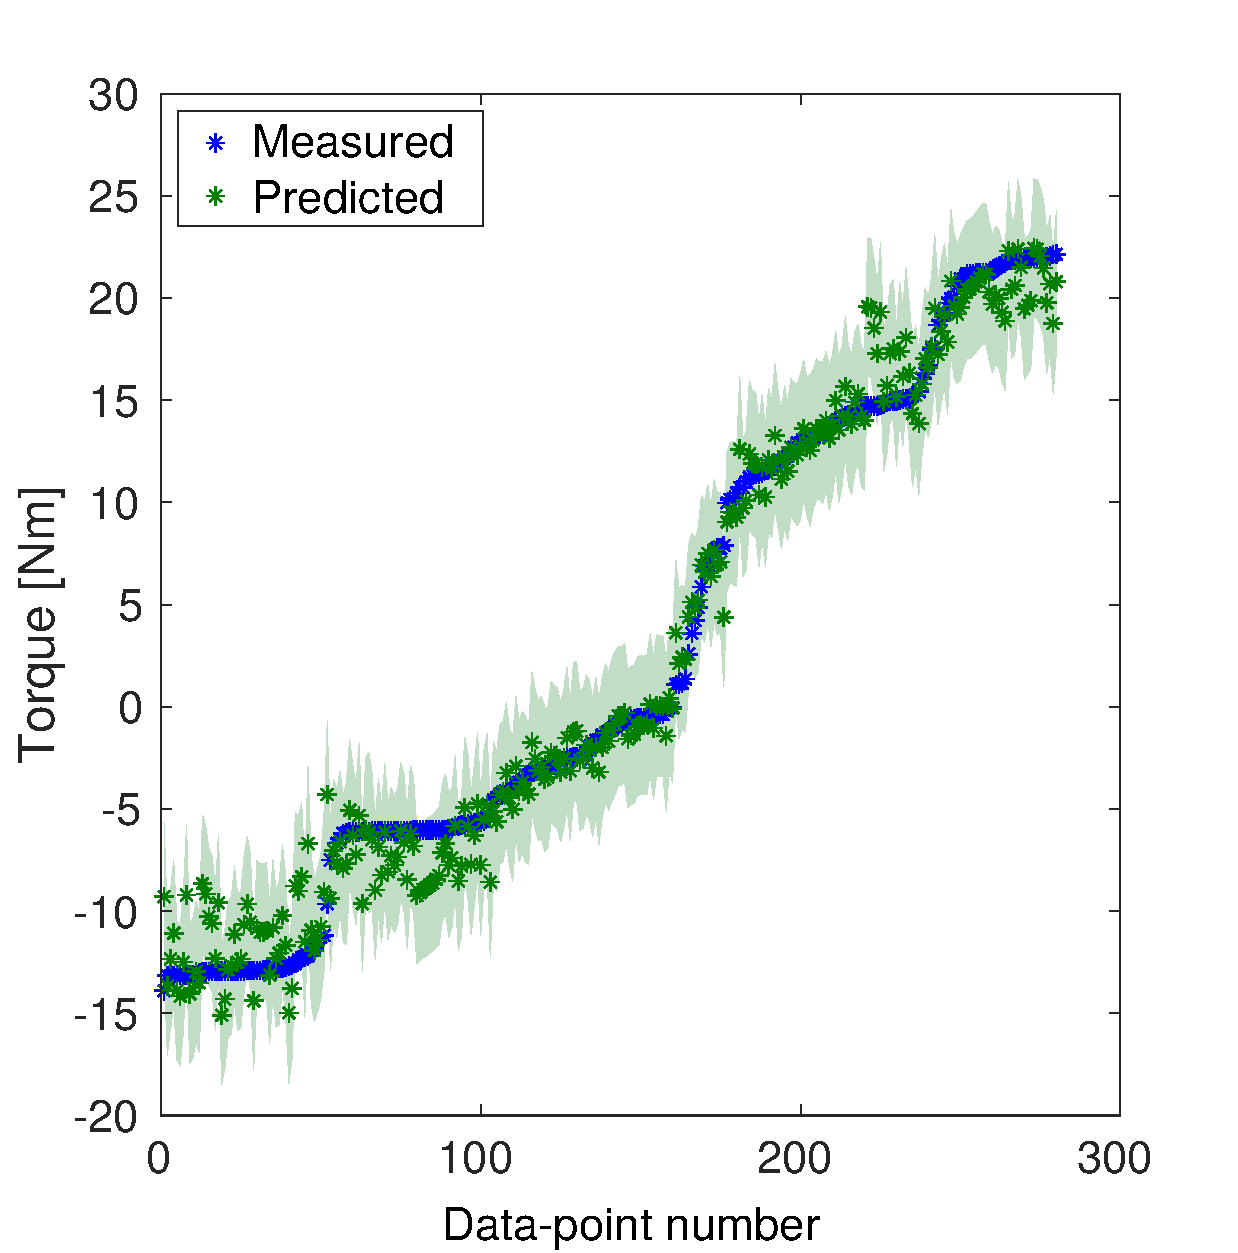
\includegraphics[width=\textwidth]{images/summer_school_study/measured_optimized_torque_A.pdf}%
    \caption{Measured values (blue) and values predicted by model A (dark green), with 95\% confidence interval (light green).}%
    \label{fig:measured_optimized_torque_A}%
  \end{subfigure}%
  \quad
  \begin{subfigure}[t]{0.48\textwidth}%
    \centering%
    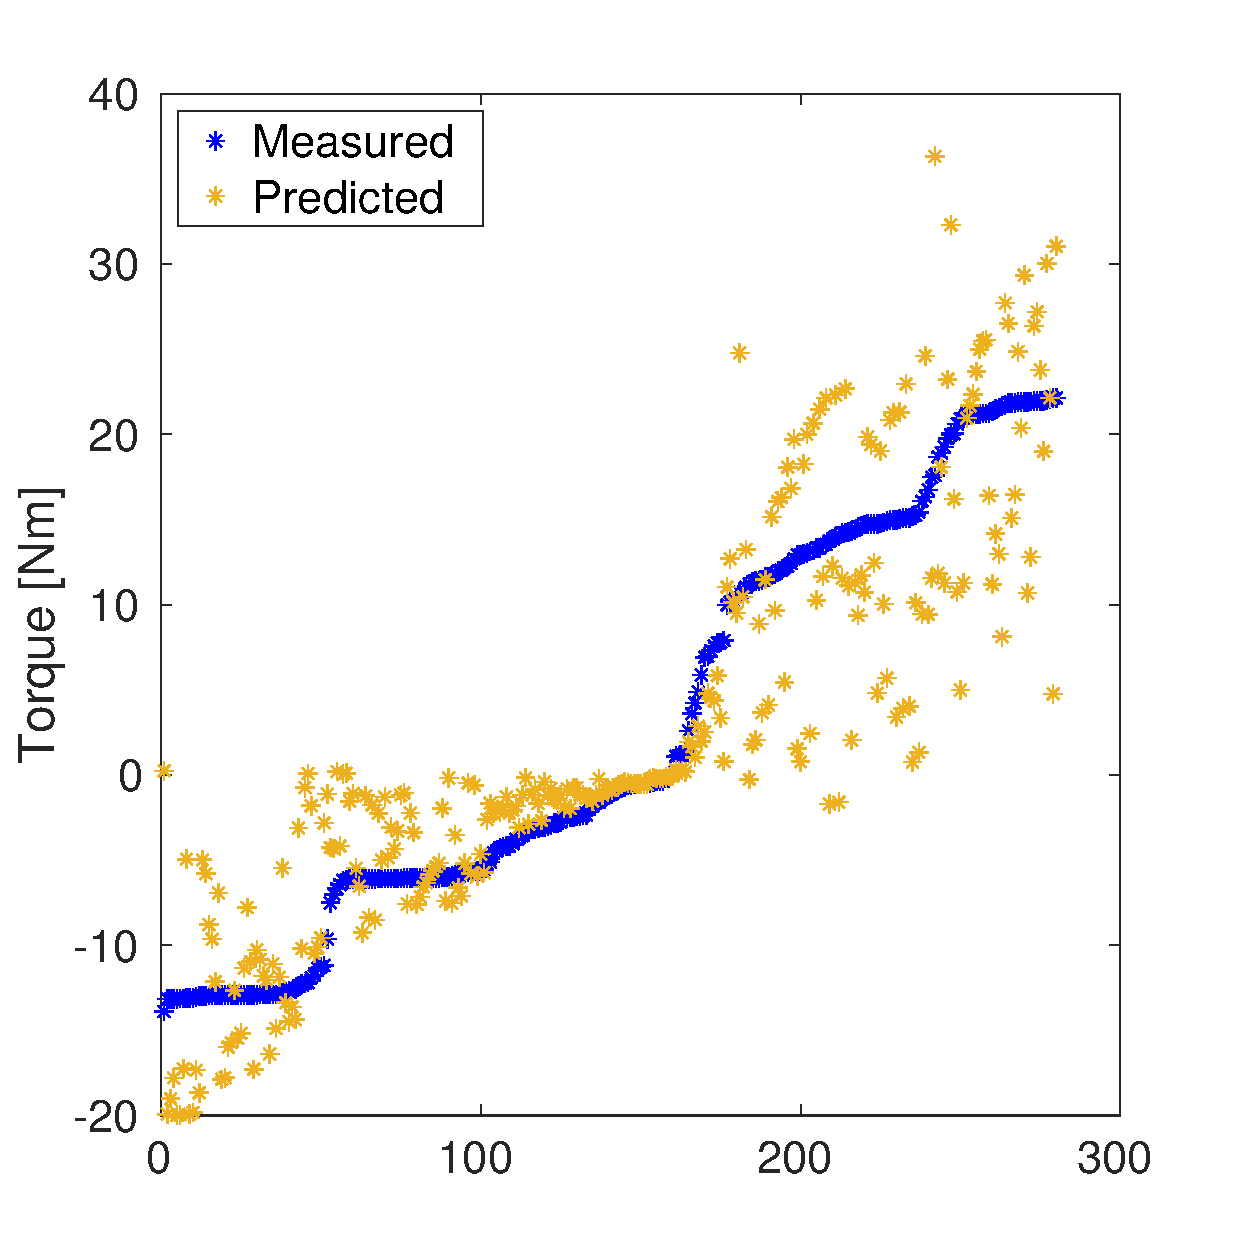
\includegraphics[width=\textwidth]{images/summer_school_study/measured_optimized_torque_B.pdf}%
    \caption{Measured values (blue) and values predicted by model B (orange).}%
    \label{fig:measured_optimized_torque_B}%
  \end{subfigure}%
  \caption{Resubstitution prediction: Measured and predicted torque values for the training data set. The measured points are ordered and numbered by magnitude, the order of the predicted points matches the order of the measured points.}%
  \label{fig:measured_optimized_torque}%
\end{figure}%

\subsection{Validation}\label{sec:res_validation}

The next evaluation uses the validation dataset and compares the predicted outputs of the models with the actual experimental values.
In contrast to the training data, where a small number $n$ of points was selected, we now use all captured values. This involves a total of \num{54e3} data points for a time span of $t=\SI{54}s$. 

\begin{figure}%
  \centering%
  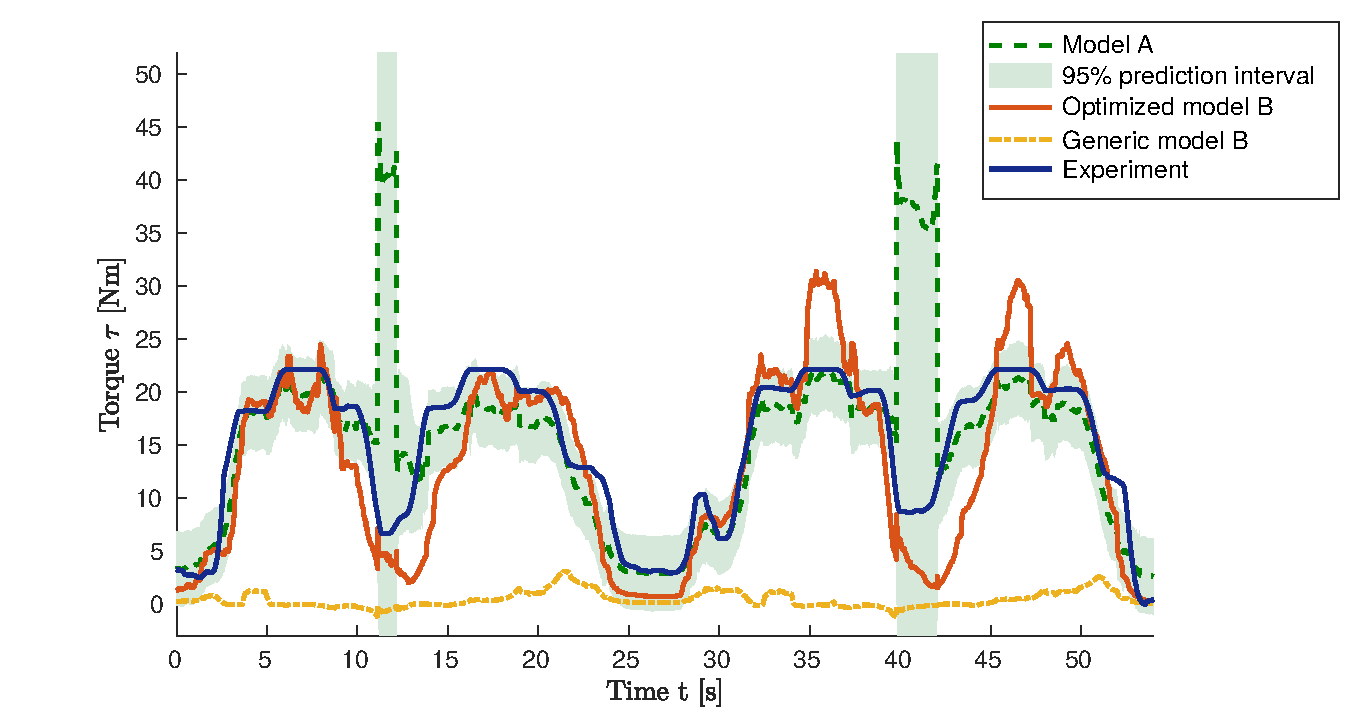
\includegraphics[width=\textwidth]{images/summer_school_study/validation_bv5_40_points.pdf}%
  \caption{Validation: Predicted torque values by model A (green), trained model B (red) and untrained model B (yellow), in comparison to the experimentally measured values (blue), for the validation data set.}%
  \label{fig:validation_bv5_40_points}%
\end{figure}%

The results are shown in \cref{fig:validation_bv5_40_points}. Comparing the green curve for model A with the blue curve for the experimental data, it can be seen that the predicted values match qualitatively for most of the time span. The predicted torque values appear consistently slightly smaller than the real values. Only for the two intervals $[\SI{11}s, \SI{12}s]$ and $[\SI{40}s, \SI{42}s]$ the predicted value is far off. The \SI{95}\percent{} confidence interval that was computed by the Gaussian Process spans a large range for these time intervals which implies that the model prediction is not to be trusted for this area. 

The biophysical model approach, model B, was tested in two variants. First, with the generic parameters from literature (yellow curve), second, with the subject-specific, optimized parameters (red curve). It can be seen that the generic model fails to predict the torque values whereas the trained model predicts reasonable values. These values are worse than most of the predictions from model A, but they succeed in giving a qualitative estimate about a low, medium or high torque output.

The match between model outputs $\tau_i$ and experimental data $\hat\tau_i$ can be quantified using the normalized root-mean-square error (NRMSE). This is a scaled version of the root-mean-square error (RMSE) and can be defined as
\begin{equation*}
  \begin{array}{lll}
    \text{RMSE} = \sqrt{\sum\limits_{i=1}^N (\tau_i - \hat{\tau_i})^2 / N},\\[4mm]
    \text{NRMSE} = \dfrac{\text{RMSE}}{\max\limits_i\{\hat\tau_i\} - \min\limits_i\{\hat\tau_i\}}.
  \end{array}
\end{equation*}
The NRMSE for model A is 0.267 which is worse than the value of 0.163 for the trained model B. The generic model B has the worst NRMSE of 0.547.

\subsection{Simplified Model A}\label{sec:res_simplified_a}
An advantage of model approach A is that it forgoes any biophysical description and the associated type of model error. It is a generic approach that does not require expert knowledge about the physiological structure. In the present study, however, some level of expert knowledge and physiological model was required in preprocessing the MoCap data, i.e. solving the inverse kinematics of the observed forearm movements to get the kinematic quantities of muscle lengths, velocities and moment arms. 

Since model A performed well in the previous validation study, we tested whether good results can also be achieved without this expert knowledge.
Consequently, the next study applies model approach A using only the elbow angle and no muscle lengths, velocities nor moment arms. Thus, the training data consists of input vectors $\bfx_i = (\phi_e(t_i), \gamma_B(t_i), \gamma_T(t_i))^\top \in \mathcal{X}$. In the following, this model is named \say{simplified model A} in contrast to the \say{full model A} that uses the complete set of input variables.

The results are shown in \cref{fig:measured_optimized_A2}. It can be seen that the resubstitution prediction in \cref{fig:measured_optimized_torque_A2} where the trained model is used to predict the training values shows a perfect fit. In contrast to the full model A, \cref{fig:measured_optimized_torque_A}, here, the learned input-output mapping shows no variance. However, the prediction for the validation dataset in \cref{fig:measured_optimized_torque_A3} shows a high error relative to the experimental data. The curve for the experimental data even lies outside the 95\% confidence interval of the prediction at some points. 

The simplified model A has a NRMSE value of 0.461. For comparison, the NRMSE values of the full and simplified model A and the generic and optimized model B are summarized in \cref{fig:nrmse}. 

This evaluation shows that simplified model A gives no useful results where the training input is too scarce. Instead, preprocessing of the measurements using a subject specific geometric model, as done for the full model A, is needed to allow for a useful prediction.

\begin{figure}%
  \centering%
  \begin{subfigure}[t]{0.48\textwidth}%
    \centering%
    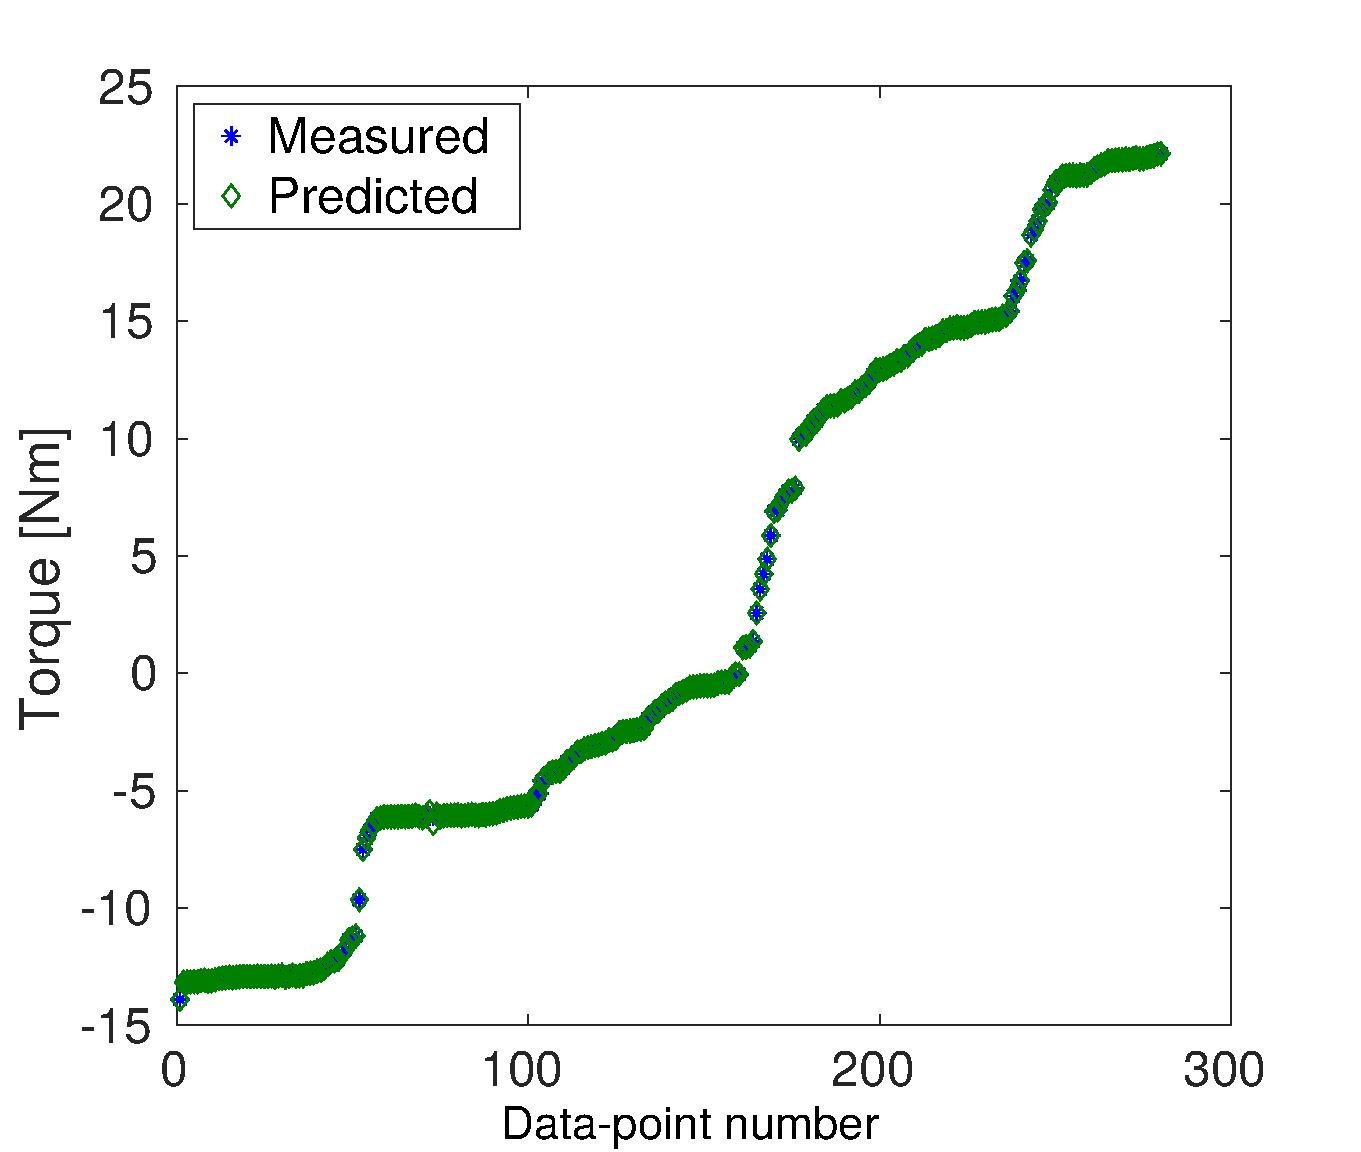
\includegraphics[width=\textwidth]{images/summer_school_study/measured_optimized_torque_A2.pdf}%
    \caption{Measured and predicted torque values of the training dataset, ordered and numbered by magnitude. The measured values (blue) and the values predicted by the Gaussian Process (green) lie on each other.}%
    \label{fig:measured_optimized_torque_A2}%
  \end{subfigure}%
  \quad
  \begin{subfigure}[t]{0.48\textwidth}%
    \centering%
    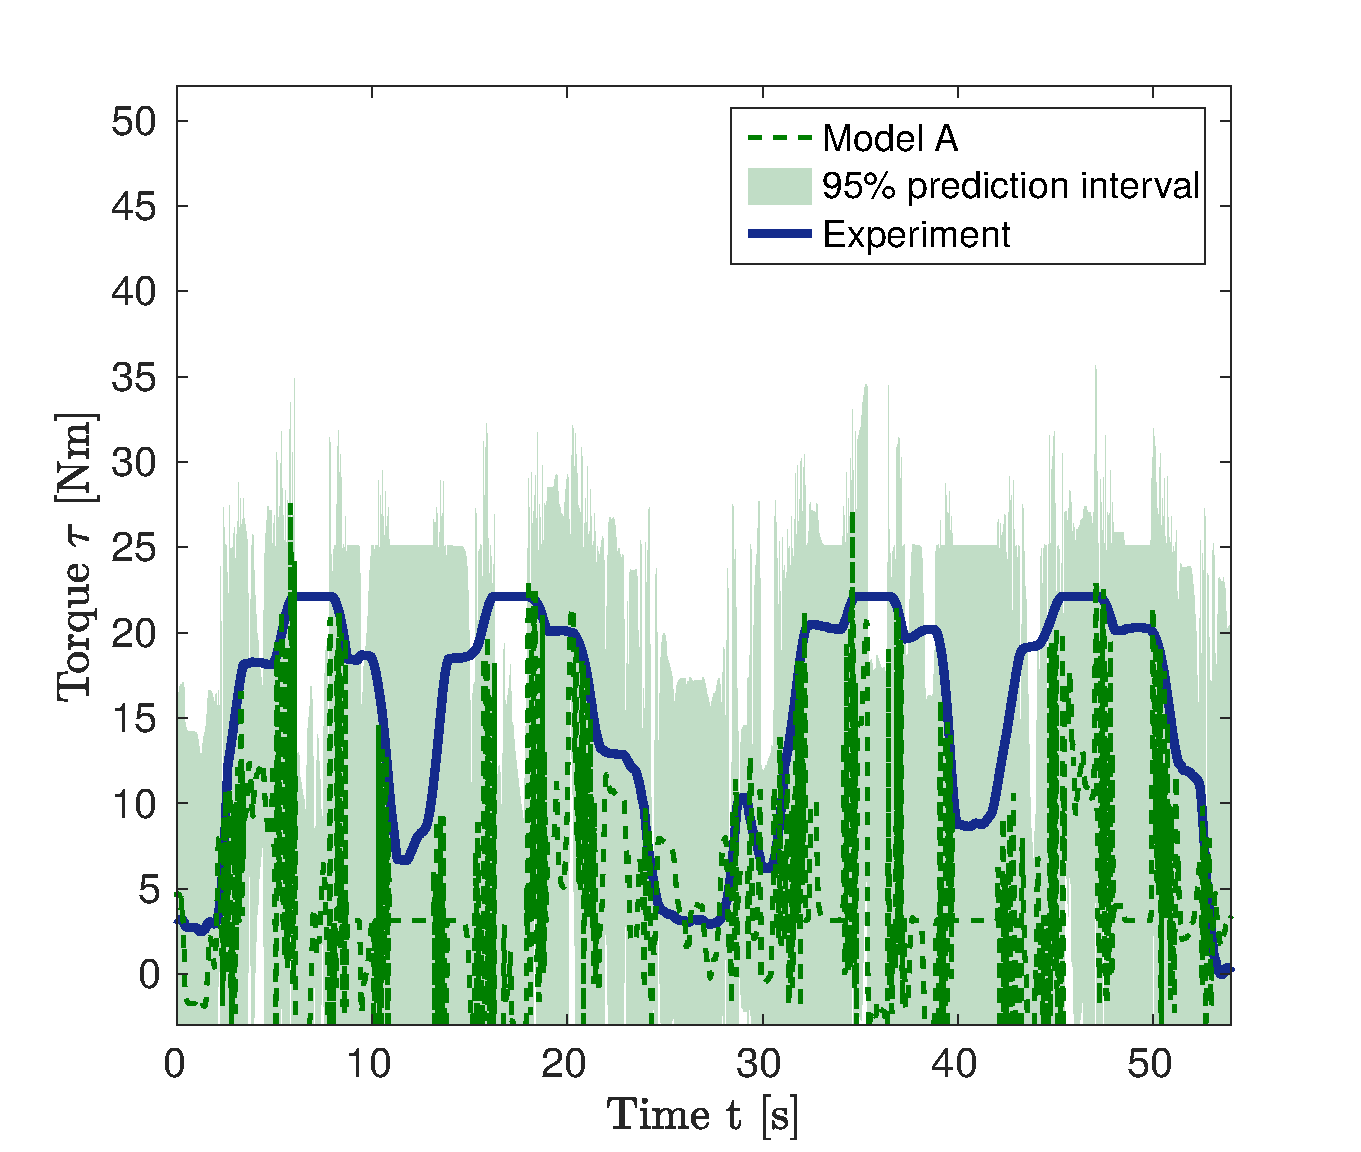
\includegraphics[width=\textwidth]{images/summer_school_study/validation_bv5_40_points_only_gamma_for_training.pdf}%
    \caption{Predicted torque values for the validation trials (green dotted line), 95\% confidence interval (light green) and the reference values of the experiment (blue). The plot reveals bad prediction capabilities of the simplified model A.}%
    \label{fig:measured_optimized_torque_A3}%
  \end{subfigure}%
  \caption{Result for the simplified model A, where, apart from the free calcium ion contractions, only the elbow angles, $\phi_e$, are used as training input instead of MTU lengths, velocities and moment arms.}
  \label{fig:measured_optimized_A2}%
\end{figure}%

\subsection{Insights of Model B}\label{ref:res_insights_b}
An advantage of model approach B is that the trained parameters are physically meaningful and allow insight into the properties of the subject specific model. Furthermore, the quality of the training data can be assessed. \Cref{fig:biceps_working_area} shows the force-length relation of the biceps muscle model using the generic and the optimized parameter values. It can be seen that the subject-specific model has a smaller slope of the force curve. 
All points of the training data set are indicated by red crosses on the curves and show the operating range of the muscle in which the model has been trained. It can be seen that the experimental training data are limited to a small range of the muscle length below its optimal CE length $l_{\CE,\text{opt}}$. In order to improve the quality of the model predictions for this subject, specific additional experimental trials can be designed for model training. They can be designed to fill in values in the missing range of operation, which in this case is for larger muscle extensions.

A low computational time of the offline parameter identification and the online evaluation of the two models would be an important measure for their practical applicability. In the present study, the training phase of Model A, i.e., optimization of the quantities for the Gaussian Process Regression using 280 training data points took \SI{2.24}{\second}. The evaluation of Model A for the validation data set containing \num{54e3} points had a duration of \SI{116}{\milli\second}.

The runtimes for model B were significantly higher. The parameter optimization lasted \SI{25}{\minute} \SI{16}{\second} and the evaluation for the validation data set had a duration of \SI{13}{\second}.

The large differences in runtime between models A and B can be explained by the inefficient implementation of the biophysical model using the MATLAB programming language. During parameter identification, this model needs to be evaluated iteratively in the optimization algorithm. In contrast, the optimization within model A works with an internal implementation of the Gaussian Process which was optimized during development of the particular MATLAB functionality.
In general, the evaluation of Gaussian Process Regression has cubic time complexity whereas, for the parameter optimization of model B, iterative solvers with linear time complexity exist.

\begin{figure}%
  \centering%
  \begin{subfigure}[t]{0.47\textwidth}%
    \centering%
    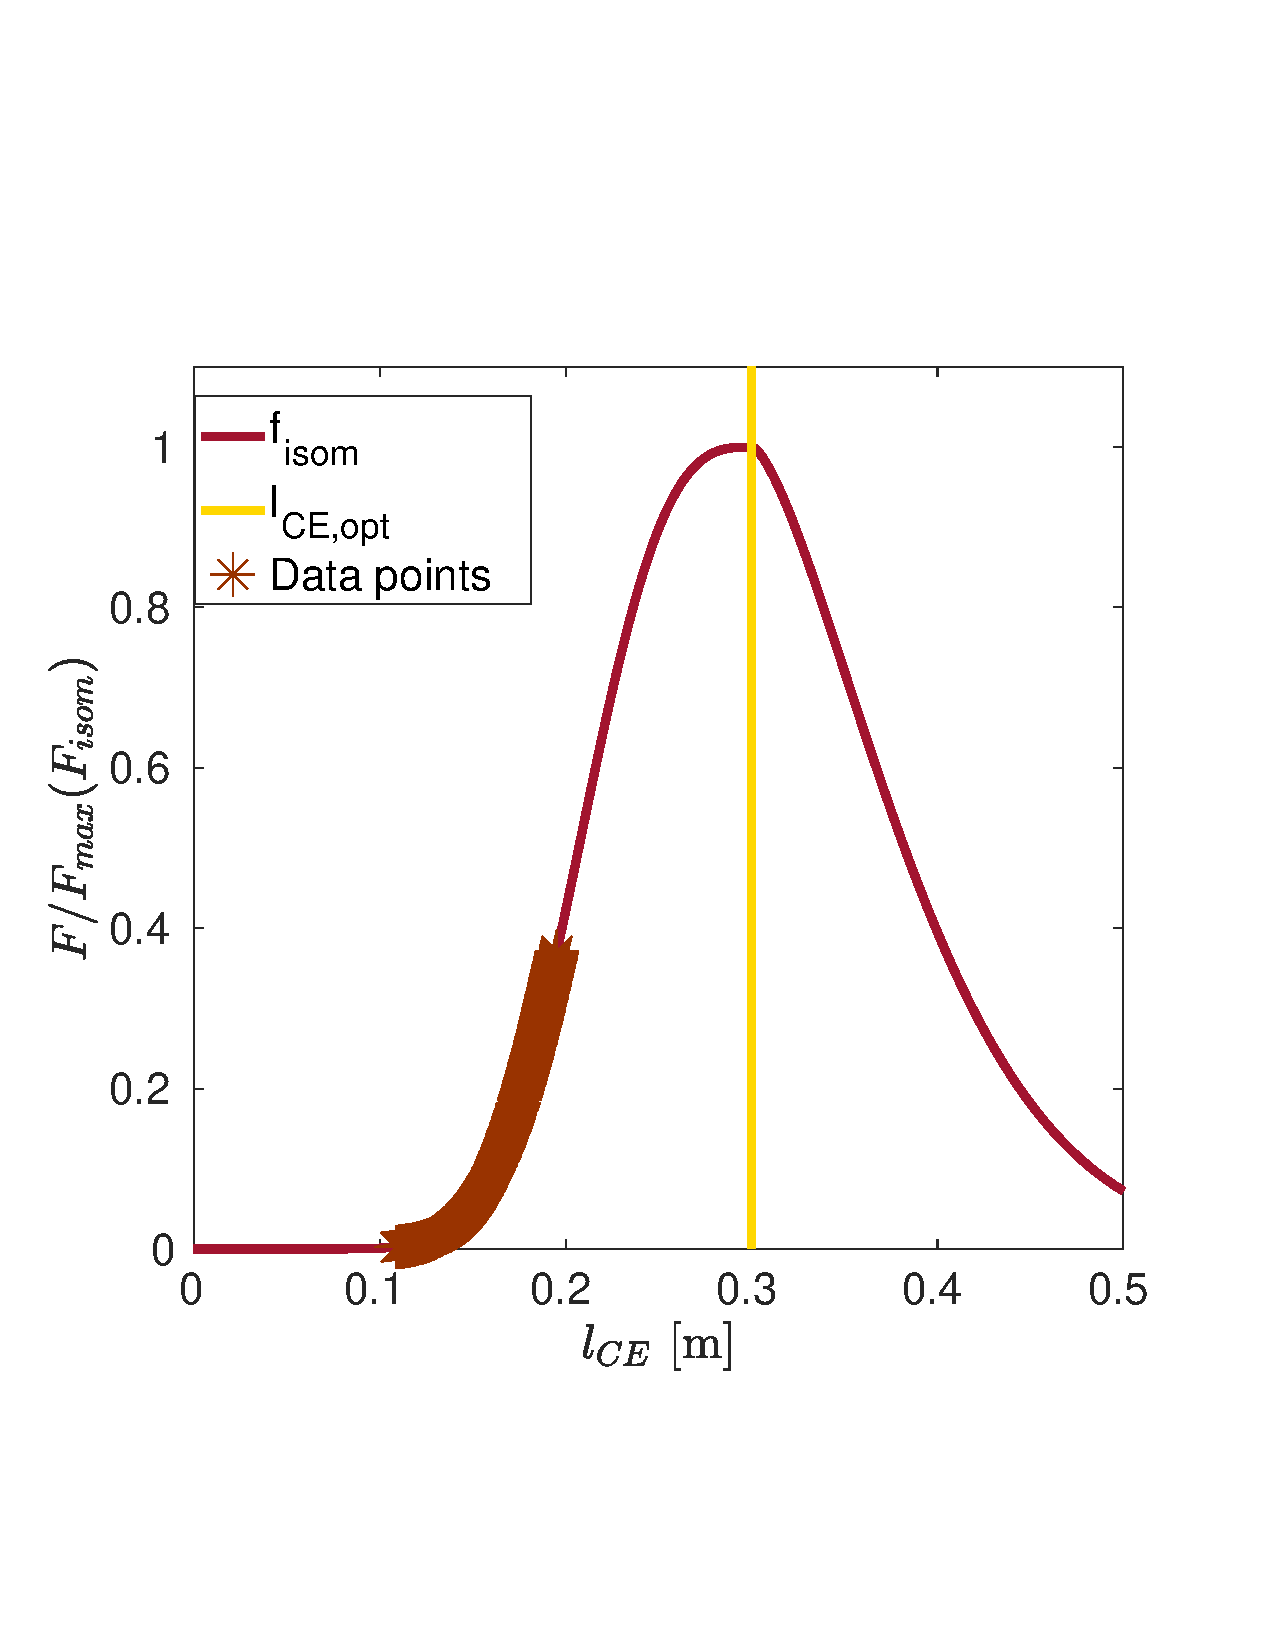
\includegraphics[width=\textwidth]{images/summer_school_study/biceps_initial.pdf}%
    \caption{Model with generic parametrization.}%
    \label{fig:biceps_a}%
  \end{subfigure}%
  \quad
  \begin{subfigure}[t]{0.47\textwidth}%
    \centering%
    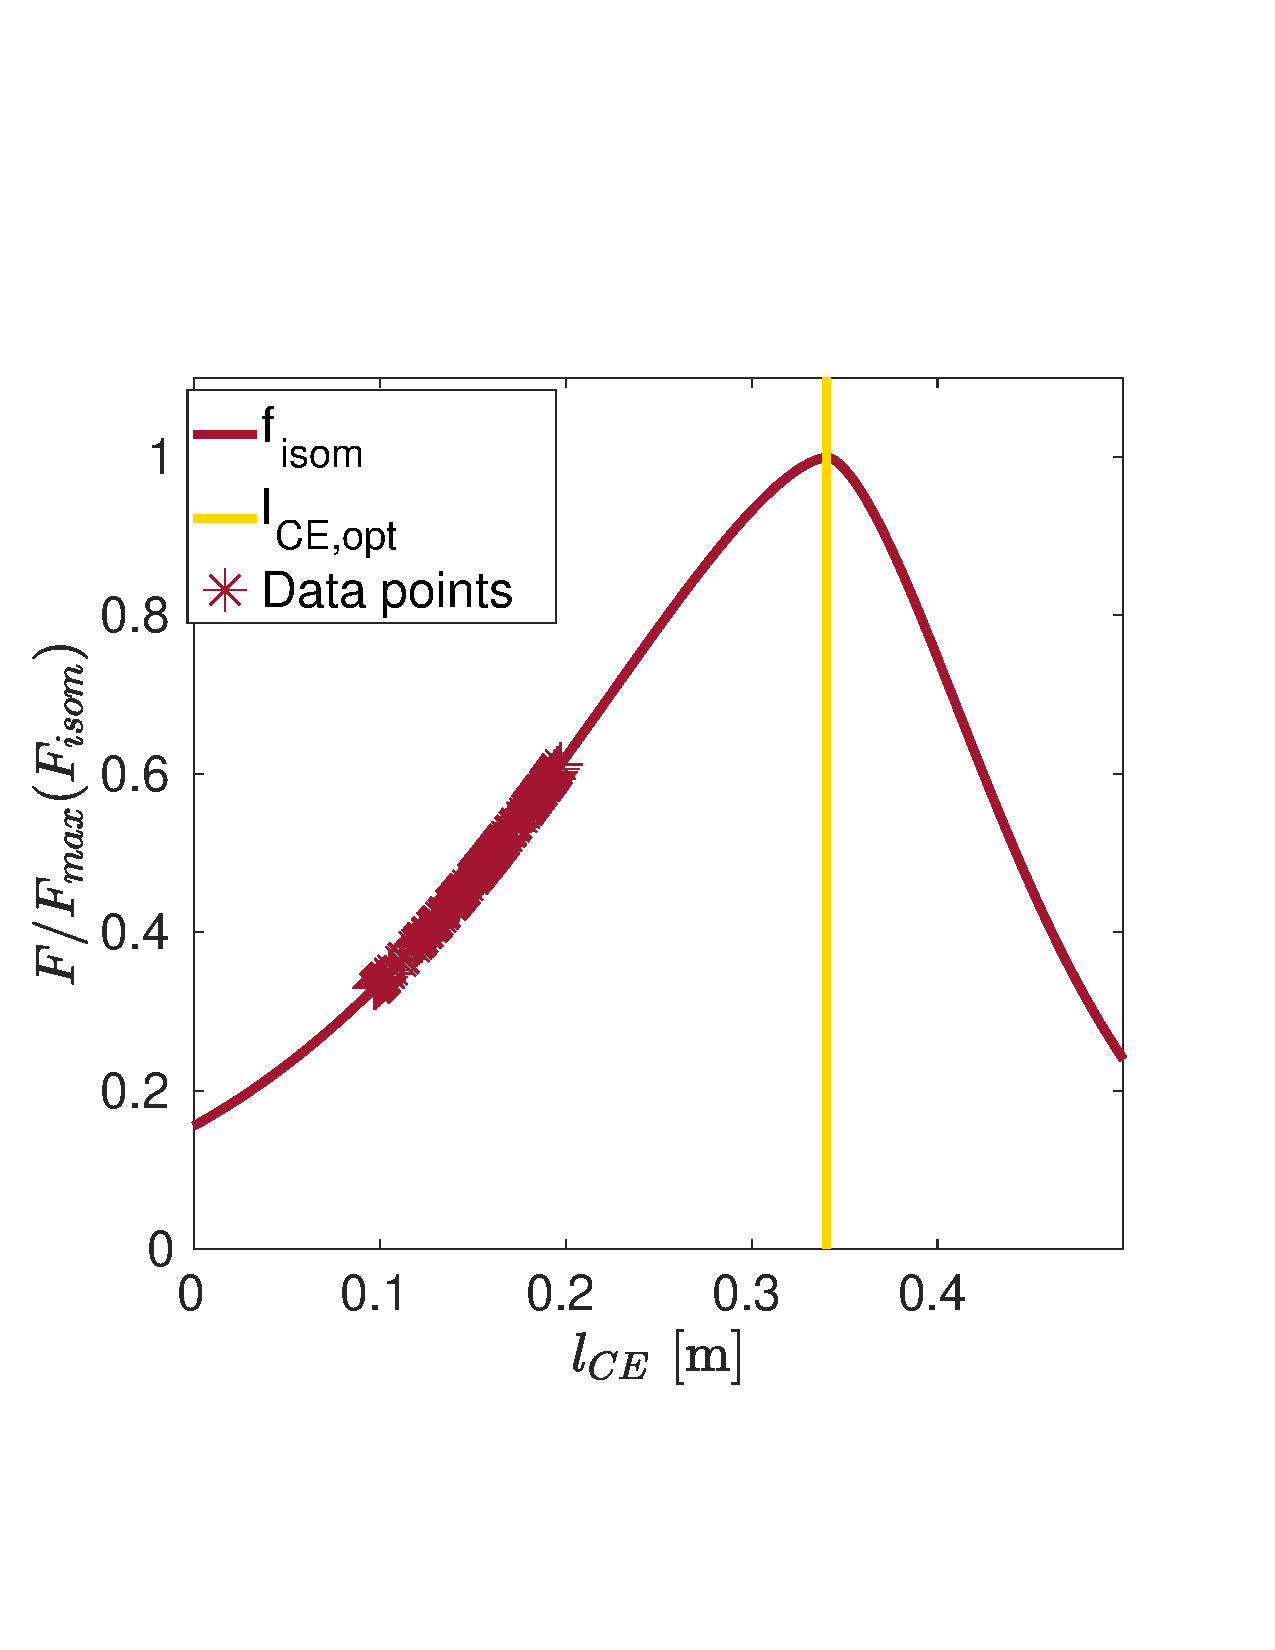
\includegraphics[width=\textwidth]{images/summer_school_study/biceps_optimized.pdf}%
    \caption{Model with subject-specific parametrization.}%
    \label{fig:biceps_b}%
  \end{subfigure}%
  \caption{Isometric force-length relation of the CE for the biceps model, analogue to \cref{fig:force_curves_generic_length}, but additionally with training data points. The points are placed on the model curve and visualize the predicted relative forces for the lengths of the CE that occurred during the training trials.}%
  \label{fig:biceps_working_area}%
\end{figure}%


\begin{figure}%
  \centering%
  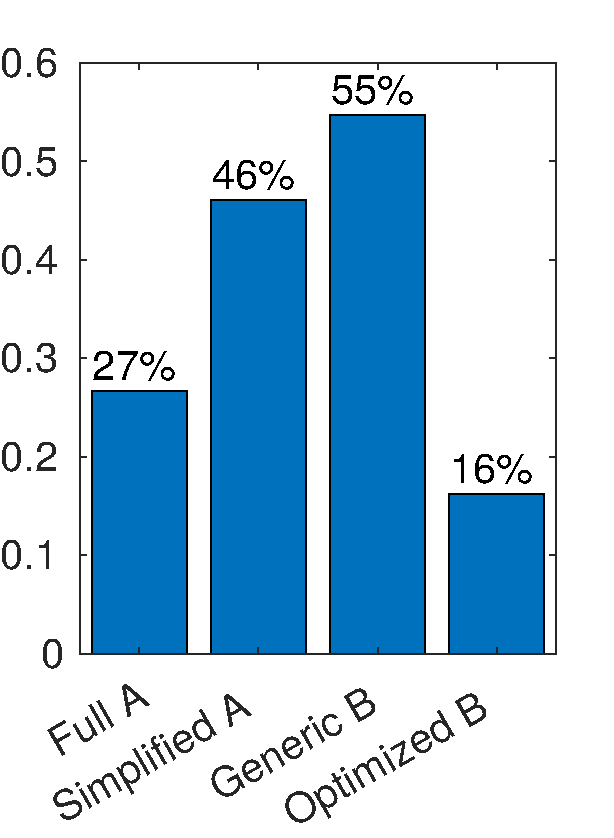
\includegraphics[width=0.35\textwidth]{images/summer_school_study/nrmse.pdf}%
  \caption{Normalized Root Mean Square errors (NRMSE) of the validation trials between the respective models and the measured values. A lower error value means a better fit.}%
  \label{fig:nrmse}%
\end{figure}%

\section{Conclusion}\label{sec:study_conclusion}
In this study, elbow torques during flexion and extension of the upper arm were predicted from motion capture data and EMG measurements. Two models, A and B, were developed. Model A is non-parametric and uses Gaussian Process Regression. Model B is biophysically informed and involves two state-of-the-art Hill-type muscle models for biceps and triceps. Experiments were conducted to generate training and validation data. These training data were used for model parameter identification. Predictions from the two models were compared to real experimental values using the validation data.

Regarding the formulation and implementation, model A requires low effort and no special knowledge about the model, except where experimental motion data is preprocessed for a specific subject. In contrast, model B needs expert knowledge about the biophysical structure and the implementation of all comprised models.

Similar holds for the offline training phase. There are no parameters in model A that have to be tuned manually, which allows a quick start. Conversely, model B requires the appropriate definition of initial values and physiological constraints for the optimization problem. However, this can also be seen as an advantage for model B, as a-priori knowledge can be integrated in such a model.

On the other hand, an advantage of model A is that additional experimental data, e.g., from neighboring muscles or additional sensors, can easily be added to the model. This is not possible with model B, where the model formulation would have to be changed.

Our studies showed that both models were able to predict the levels of torque reasonably. 
\Cref{fig:nrmse} showed the best score for model A, followed by model B. It was also seen that the generic parametrization of model B does not yield a useful prediction. The same is true for a simplified version of model A, where the elbow torque was used as training input instead of derived quantities from the motion capture system that required a complex preprocessing step.

Both models provide possibilities to assess the confidence of their predictions. With model A, confidence intervals can be computed directly from the Gaussian Processes. Their usefulness was shown in the validation where regions with large errors also had a large confidence interval. 
Model B allows insight into force-length and force-velocity characteristics of the two involved muscles. The operating ranges of the muscles during the experiments can be visualized and allow assessing whether the desired model features were covered by the training phase and, thus, will yield a good prediction.

In our study, runtimes were low for model A and high for model B in both offline and online phases. However, this is due to our prototypical implementation of model B. For larger data sizes and a more sophisticated implementation, the reverse effect is expected. The runtime complexity for the training phase is better for model B (linear in time) compared to model A (cubic in time). For the online phase, costly integration over data points is needed for model A whereas model B directly provides a differential equation of the system that can be solved efficiently. 

If EMG is used to control an exoskeleton that supports the movement of the limb, it is known that the measured signals are ahead of the intended movement by a small offset. This is a result of the time delay in the neuromusculoskeletal system. This property gives the assistive exoskeleton a short time to predict the intended movement and thereby allows a seamless integration of the artificial device with human control.

When targeted at such a real-time application, both models could be considered to be integrated into the control. Model A better fits the use case of a device that could be (re\nobreakdash-)calibrated by the patient itself. Because of the built-in estimation of prediction quality, compliance and safety could be ensured more easily even for imperfect training.
Model B would need a controlled environment such as a specialist's laboratory and careful assistance for the calibration process.
After calibration, it would promise a more natural and more responsive experience because of the subject-specific model and possibly smaller compute times.

Where real-time application is not a requirement, biophysically informed models have a high potential to leverage the understanding how the human neuromusculoskeletal system operates for given tasks.
In model B of this study, the kinematics and individual muscle dynamics were described close to the current  understanding of the system. However, several aspects where not modeled as detailed as possible. The pathway from neural stimulation to excitation and activation of the muscle, the recruitment strategies including different motor units, neural feedback loops as well as effects stemming from the 3D geometry of the muscle were not considered. Therefore, this thesis develops a more detailed, biophysically informed model including these properties in the following chapters.

The presented study reproduced what similar studies in literature have shown: Subject-specific model identification for Hill-based torque prediction models can vastly improve the prediction quality compared to generic models. Our work adds to the common knowledge that this holds also for the four-element Hill-type model that was used for model B. Furthermore, a comparison with Gaussian Process Regression was given, various advantages and disadvantages of these two approaches were identified. Future work can test the two models with more subjects and increase the variety of motion in the training experiments. For example, effects resulting from high contraction velocities or eccentric contractions could be investigated to evaluate the model's potential in more complex movements.


% \chapter{Formulation of electrophysiology and muscle contraction}
%    - electrophysiology introduction
%    \section{State of the art}
%    - Hodgkin-Huxley, shorten, advanced models, how it gets solved
%    \section{discretization}
%    - discretization of electrophysiology, operator splitting
%    \section{Standard for formulation of models}
%    - cellml introduction
%    \section{Bidomain}
%    - EMG
%    \section{Multidomain}
%    - multidomain formulation
%    \section{Formulation of solid mechanics}
%    - basics solid mechanics framework, material modeling, 
%    
%    \section{Simulation workflow}
%    - simulation workflow of skeletal muscle
%  
% \chapter{Numerics}
%   \section{Fundamentals of the discretization}
%    \section{Finite element method}
%    - basics FEM formulation of Laplace operator and diffusion equation, boundary conditions
%    \section{Incompressible nonlinear solid mechanics}
%    - incompressibility, penalty formulation vs. mixed formulation\\
%    - governing nonlinear eq.\\
%    - jacobian
%   \section{Numerical schemes}
%    \section{time stepping schemes}
%    \section{linear system solvers}
%    \section{newton algorithm}
%  % 
% \chapter{Simulation software}
%    \section{State of the art}
%    - review on bioengineering simulation frameworks 
%    
%    \section{OpenCMISS}
%  - OpenCMISS introduction, iron zinc cmgui, unstructured\\
%  
%  - Strang splitting, solvers 1D\\
%  - improved interpolation\\
%  - parallelization, issue with 1D \\
%  - 3D parallelization strategies\\
%  - design flaws, memory\\
%    % untergliedern, z.B. schnittstellen parall etc.
%    \section{The simulation framework \emph{opendihu}}
%    - modularity of opendihu, concepts (python c++ build system)
%    \section{Overview of discretization features}
%    - feature overview, implemented equations, ansatz functions, meshes
%    \section{Input and output}
%    - file i/o parallel, i: only local data important for high parallelism, o: paraview
%    \section{In-situ visualization}
%    - in-situ
%    \section{Details on the implementation}
%    \section{Representation of structured meshes}
%    \section{Parallel data handling}
%    - data structures, petsc variables, partitioning, ghost communication
%    \section{Implementation of boundary conditions}
%    - Neumann, Dirichlet boundary conditions
%    \section{Implementation of material formulation and automatic derivation of derivatives}
%    - implementation of solid mechanics with analytic differentiation
%    
%    \section{efficient and configurable data transfer}
%    - data layout details, efficient transfer of variables between solvers
%    \section{Mapping between meshes}
%    - parallel mapping between meshes, invertability of index space represesantion
%    \section{An efficient solver to the Monodomain equation}    
%    - cellml code generator and its optimizations - openmp, simd, vc
%    \section{Details on the partitioning}
%    - fibers emg structure and partitioning
%    \section{Parallelization of the multidomain system}
%    - multidomain parallelization, reordering of matrix
%    \section{load balancing}
%    - load balancing on fiber level
% \chapter{External coupling}
%    - introduction to external coupling, precice
%    \section{coupling with FEBio}
%    \section{coupling with AceFEM}
%  
\chapter{Generation of Meshes}

The formulations of electrophysiology and contraction of tendon and muscle tissue are given on different domains.
The muscle belly forms the domain $\Omega_M$. A layer of fat and skin tissue on top of the muscle is denoted the body domain $\Omega_B$.
On both longitudinal ends, the muscle is attached to tendons, given by the domains $\Omega_{T,1}$ and $\Omega_{T,2}$.

All these domains are placed in the 3D Euclidean space, $\Omega_M,\Omega_B,\Omega_{T,i} \subset \R^3$.
Additionally, formulation of electrophysiology on individual muscle fibers need one-dimensional domains $\Omega_{F,i} \subset \R^3$ for $i \in \{0,\dots,n_f\}$. In such formulation, the whole muscle typically consists of a large number $n_f$ of these fiber domains.
Each domain $\Omega_{F,i}$ is a 1D manifold embedded in the 3D domain. The domains are visualized in \cref{fig:fibers_domains}.

\begin{figure}%
    \centering%
    \def\svgwidth{8cm}%
    \input{images/fiber_creation/domains.pdf_tex}%
    \caption{Visualization of the computational domains: tendons $\Omega_{T,1}, \Omega_{T,2}$, muscle belly $\Omega_M$, body domain $\Omega_B$ and fiber domains $\Omega_{F,i}$.}%
    \label{fig:fibers_domains}%
\end{figure}%

For discretization using the Finite Element Method, we approximate the 3D domains and 1D manifolds, $\Omega_\text{3D}$ and $\Omega_\text{1D}$, 
by a number of 3D elements $\{U_{\text{3D},i}\}_{i=1,\dots,n}$ with $U_{\text{3D},i} \subset \R^3$, respective 1D elements $\{U_{\text{1D},i}\}_{i=1,\dots,n}$, with $U_{\text{1D},i}\subset \R^3$.
An element is given by a number of nodes and their connectivity information. Their disjoint union approximates the overall computational domain,
 $\dot{\bigcup}_{i=1}^{n} U_\text{3D} \approx \Omega_\text{3D}$ and $\dot\bigcup_{i=1}^{n} U_\text{1D} \approx \Omega_\text{1D}$.

The elements can be defined by a mesh. In this section, structured meshes are assumed. 
A 3D structured mesh is homomorphic to a 3D regular cartesian grid. 
The number $n$ of elements is the product of the numbers $n_i, n_j$ and $n_k$ of elements in the three coordinate directions $x,y$ and $z$ of the regular cartesian grid,
 i.e., $n = n_i\,n_j\, n_k$.
Each element can be indexed by a triple $(i,j,k)$ of indices with the ranges $i \in \{0,\dots,n_i-1\}, j \in \{0,\dots, n_j-1\}$ and $k \in \{0,\dots,n_k-1\}$. 
In the program, typically, consecutive indices $\iota$ are used that iterate over all elements $\iota \in \{0,\dots,n-1\}$ and are obtained from the index triples by the mapping 
$(i,j,k) \mapsto \iota = k\,n_i\,n_j + j\,n_i + i$.

The elements can have different numbers of nodes, depending on the spatial order of consistency of the discretization. 
In this section, only 1D elements with two nodes and quadrilaterial 3D elements with $2^3=8$ nodes are considered. 
Higher order elements can be composed geometrically by using the nodes of the respective number of adjacent elements in the structured mesh.
For this purpose, we always generate 3D meshes with an uneven number of elements in the coordinate directions. 
Thus, linear elements with eight nodes or quadratic elements with 27 nodes can be created from the same global set of nodes.

In the following, algorithms for the generation of the needed meshes are presented. 
The requirement is to construct a 3D structured mesh that fills a given volume. This is needed for the muscle and tendon domains, $\Omega_M$ and $\Omega_{T,i}$.
Additionally, for the 3D muscle domain, a specified number of 1D muscle fiber meshes that are embedded in the 3D mesh have to be created. 
The fibers should be positioned to match the anatomy of the muscle. For the biceps and triceps muscles with their fusiform layout,
a streamlined orientation of the fibers is needed.

% overview subsections

\section{Related Works}

\section{Preprocessing of the Muscle Geometry}

The first step towards creating a structured mesh is to obtain a representation of the surface of the muscle. 
Starting point is a human biomedical imaging data set. In this section, two possible workflows are presented how to extract the muscle and tendon surface. 
The two workflows are visualized in \cref{fig:scheme_preprocessing}. The workflow using the branch on the left side in \cref{fig:scheme_preprocessing} is automized but only works for the particular data set and extracting the biceps muscle.
The right branch involves manual steps and is applicable for any muscle geometry.

% overview over subsections

\begin{figure}%
  \centering%
  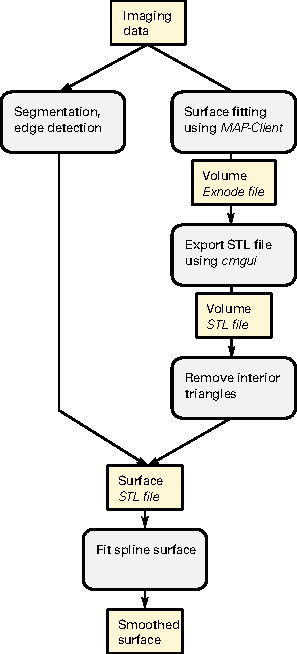
\includegraphics[height=15cm]{images/fiber_creation/scheme_preprocessing.pdf}%
  \caption{Workflow of generating a surface representation of the muscle and tendons from imaging data. Intermediate results are visualized as yellow boxes. Two possible branches are shown. On the left, the imaging data is processed using automatic processing to directly retrieve points on the surface of the muscle. On the right, the same is achieved with three steps of which the first one involves manual adjustments. At the end, a spline surface smooths the collected data from both possibilities to yield the resulting surface representation.}%
  \label{fig:scheme_preprocessing}%
\end{figure}%

\subsection{Data source}
Anatomic images provide the basis for the extraction of muscle geometries.
The used data set originates from the Visible Human Project \cite{visible_human_male} of 
the United States National Library of Medicine. 
The project has published anatomic images derived from a male cadaver, among other data sets.
The data, known as \say{Visible Human Male}, were published in 1994.
Colored images of transversal cross sections were obtain by cryosectioning.
A total of \num{1871} images with dimensions of \num{2048} by \num{1216} pixels and 24 bit color depth visualize the whole human body. Parts of the upper arms are contained in approximately 500 of these images. The size of a pixel is \SI{0.33}{\milli\meter} in transversal direction and \SI{1}{\milli\meter} in axial direction. The size of the complete set of JPEG compressed images is \SI{772}{\mega\byte}. Cropping and selecting the relevant portions of the upper arm extracts a dataset with the size of \SI{35}{\mega\byte}.

An extract of an image of the upper arm is given in \cref{fig:vhp_image}. 
Biceps and triceps brachii muscles can be identified as the dark red tissue. For the biceps, the two muscle heads are visible, separated by the bright diagonal line from bottom left to top right. For the triceps, at least two of the three heads can be identified. The blue background is colored frozen gelatin that was needed during cryosection to stabilize the arms.

\begin{figure}%
  \centering%
  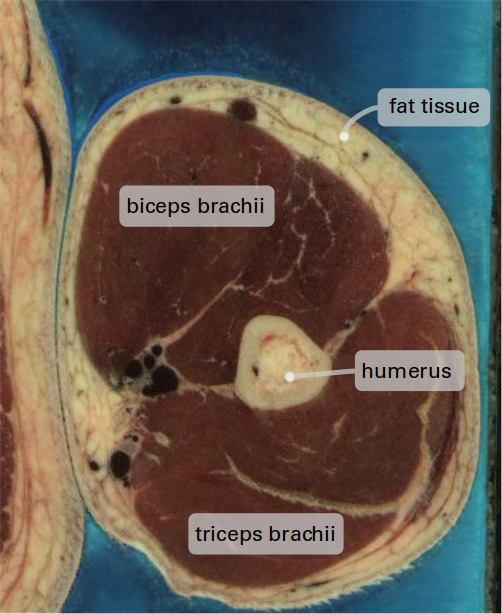
\includegraphics[height=10cm]{images/fiber_creation/vhp.png}% 0483
  \caption{Exemplary extract of image number 483 from the Visible Human Male. A transversal slice of the left upper arm is shown as seen from the bottom. The biceps and triceps muscles as well as the humerus bone can be identified. }%
  \label{fig:vhp_image}%
\end{figure}%

\subsection{Automatic surface extraction}
This section outlines the automatic algorithm to obtain the muscle surface from the Visible Human Male data set. The scheme corresponds to the left branch in \cref{fig:scheme_preprocessing}. The algorithm was implemented as Python script as part of the Bachelor thesis of Kusterer \cite{Kusterer} that was supervised by me.
The algorithm is capable of extracting muscle and bone geometries from the described imaging data.

At first, the color values of the images are used to segment the imaging data into muscle tissue, surrounding tissue and skeletal structure. The algorithm traverses the selected and cropped relevant parts of the images. For example, to segment the biceps muscle, the image region of pixels coordinates $(x,y)$ with $x \in [1300,1720] $ and $ y\in[1030,1720]$ are considered in the images with numbers 284 to 778. 

For every such part of an image, pixels that match a certain range in the RGB color space are marked and categorized. The categories are muscle tissue and, for comparison, also bone tissue. The corresponding color ranges are given in \cref{tab:color_ranges}.
This color based classification does not succeed everywhere as the white shade corresponds not only to bone material but also to fat and other tissue. Therefore, the algorithm removes artifacts located near the outer gelatine from the set of pixels categorized as bone. 

\begin{table}
  \centering%
  \begin{tabular}{l|lll}
    \hline
    & red & green & blue\\
    \hline
    muscle & $60 - 100$& $30-75$   & $15-60$\\
    bone   & $145-255$ & 1$35-205$ & $60-160$\\
    \hline
  \end{tabular}
  \caption{Ranges in the RGB color space to identify pixels of muscle and bone segments. The numbers correspond to 24 bit colors with the range $[0,255]$ for every color channel.}%
  \label{tab:color_ranges}%
\end{table}

Exemplary results for image number 483 are given in the left column of \cref{fig:vhp_image}.
It can be seen that the marked regions for muscle and bone have gaps in the interior resulting from differently colored tissue inside muscles and bones. On some images, the set of pixels also includes small objects outside the actual muscle and bone regions.

To reduce the gaps and small objects, the morphological operations \emph{closing} and \emph{opening} are performed on the data. These operations consist of \emph{dilation} and \emph{erosion} steps. Both are pixel based operations that traverse the dataset and for every pixel consider a window of $3\times 3$ pixels centered at the current position. Dilation picks the maximum value and erosion the minimum value from this window and assigns it as the pixel's value in a new image. In our case, values of zero and one correspond to non-categorized and categorized pixels, respectively.

Closing consists of dilation followed by erosion and closes small gaps or holes in the marked objects. Opening consists of erosion followed by dilation and removes small artifacts outside the actual bone and muscle areas. It was found effective to perform each dilation and erosion twice in sequence to yield good results with almost no more holes and unwanted small objects.

Next, the algorithm determines the contours of all regions with marked pixels. This leads to lines with a width of one pixel that enclose the muscle and bone areas. The right column of \cref{fig:extraction} shows the results after this step. It can be seen that the morphological operations close numerous gaps. In some images, as in the considered example, the muscle area gets split into multiple smaller enclosed regions which is not desired. However, proper contours of the biceps are found in the majority of images. 

\fboxsep=0mm   % padding thickness
\fboxrule=1pt   % border thickness
\begin{figure}%
  \centering%
  \fcolorbox{black}{black}{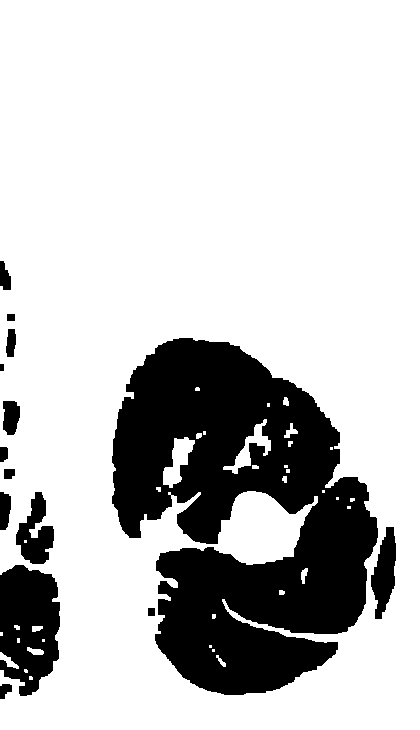
\includegraphics[height=7cm,trim=0 0 0 6cm, clip]{images/fiber_creation/extraction_segmentation_482.png}}\quad%
  \fcolorbox{black}{black}{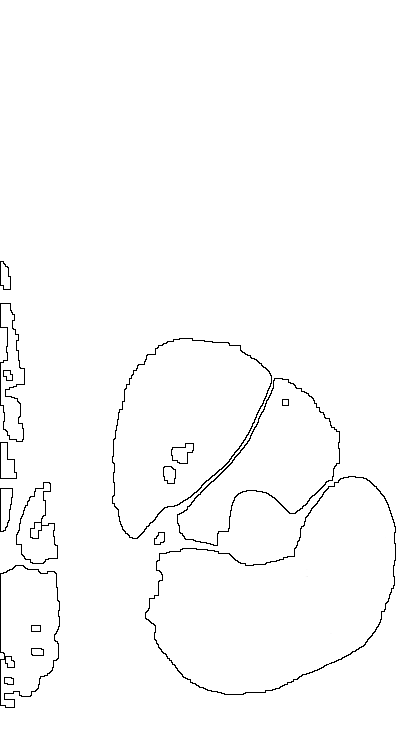
\includegraphics[height=7cm,trim=0 0 0 4cm, clip]{images/fiber_creation/extraction_contour_482.png}}\vspace*{5mm}\\
  \fcolorbox{black}{black}{
\includegraphics[height=7cm,trim=0 0 0 6cm, clip]{images/fiber_creation/extraction_bone482.png}}\quad%
  \fcolorbox{black}{black}{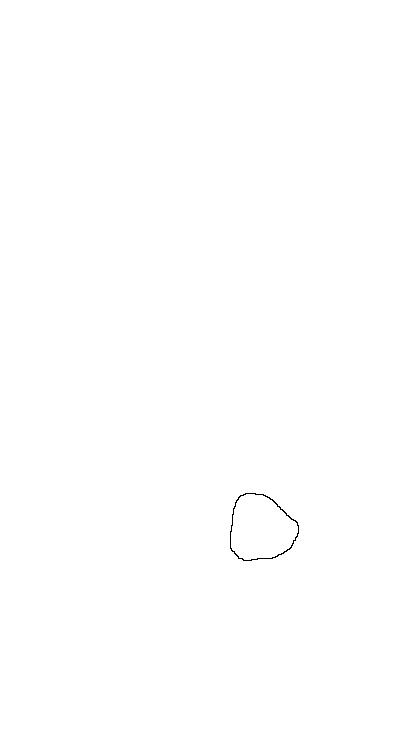
\includegraphics[height=7cm,trim=0 0 0 6cm, clip]{images/fiber_creation/extraction_surface_bone482.png}}%
  \caption{Intermediate steps of the algorithm to determine surface geometry of muscles and bones. The left columns shows pixels from the image in \cref{fig:vhp_image} that were categorized to be muscle tissue (top) and bone material (bottom). The right column shows a later step in the algorithm, where the surface of muscle (top) and bone (bottom) is estimated.}%
  \label{fig:extraction}%
\end{figure}%

In the next step, a single contour for each of muscle and bone is obtained in every image. If there are multiple contours per image, the one that is located the most in upper right location within the image is selected for the muscle. If all contours in an image are shorter than 20 pixels, this is a sign of bad segmentation quality and the whole image gets discarded.

The result is a set of contours for muscle and bone in the cross-sectional planes of the images. Combining these, we get a point cloud in 3D space that approximates the surface of the biceps muscle and the surfaces of the considered bones humerus, ulna and radius. Using these points, a spline surface can be fitted and subsequently triangulated. Resulting surfaces for the biceps and humerus bones are shown in \cref{fig:extraction_result}.
%
\begin{figure}%
  \centering%
  \begin{subfigure}[t]{0.48\textwidth}%
    \centering%
    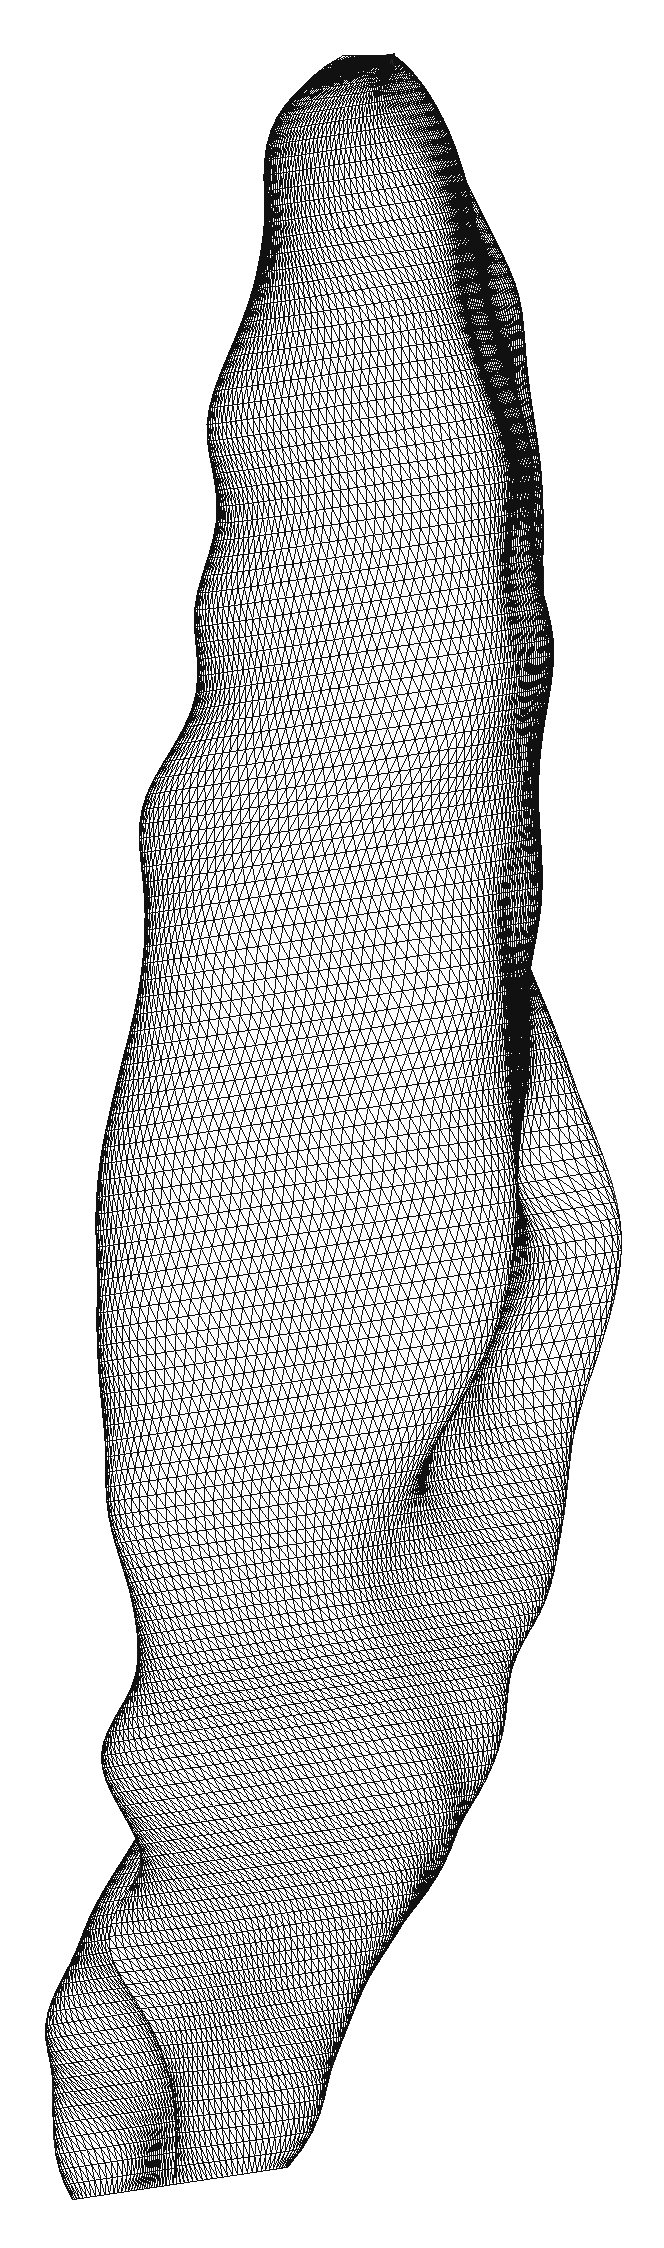
\includegraphics[height=6cm]{images/fiber_creation/extraction_biceps.png}%
    \caption{Surface of the biceps brachii muscle. At the right side of the muscle, the groove of the humerus bone can be seen.}%
    \label{fig:extraction_result_biceps}%
  \end{subfigure}
  \begin{subfigure}[t]{0.48\textwidth}%
    \centering%
    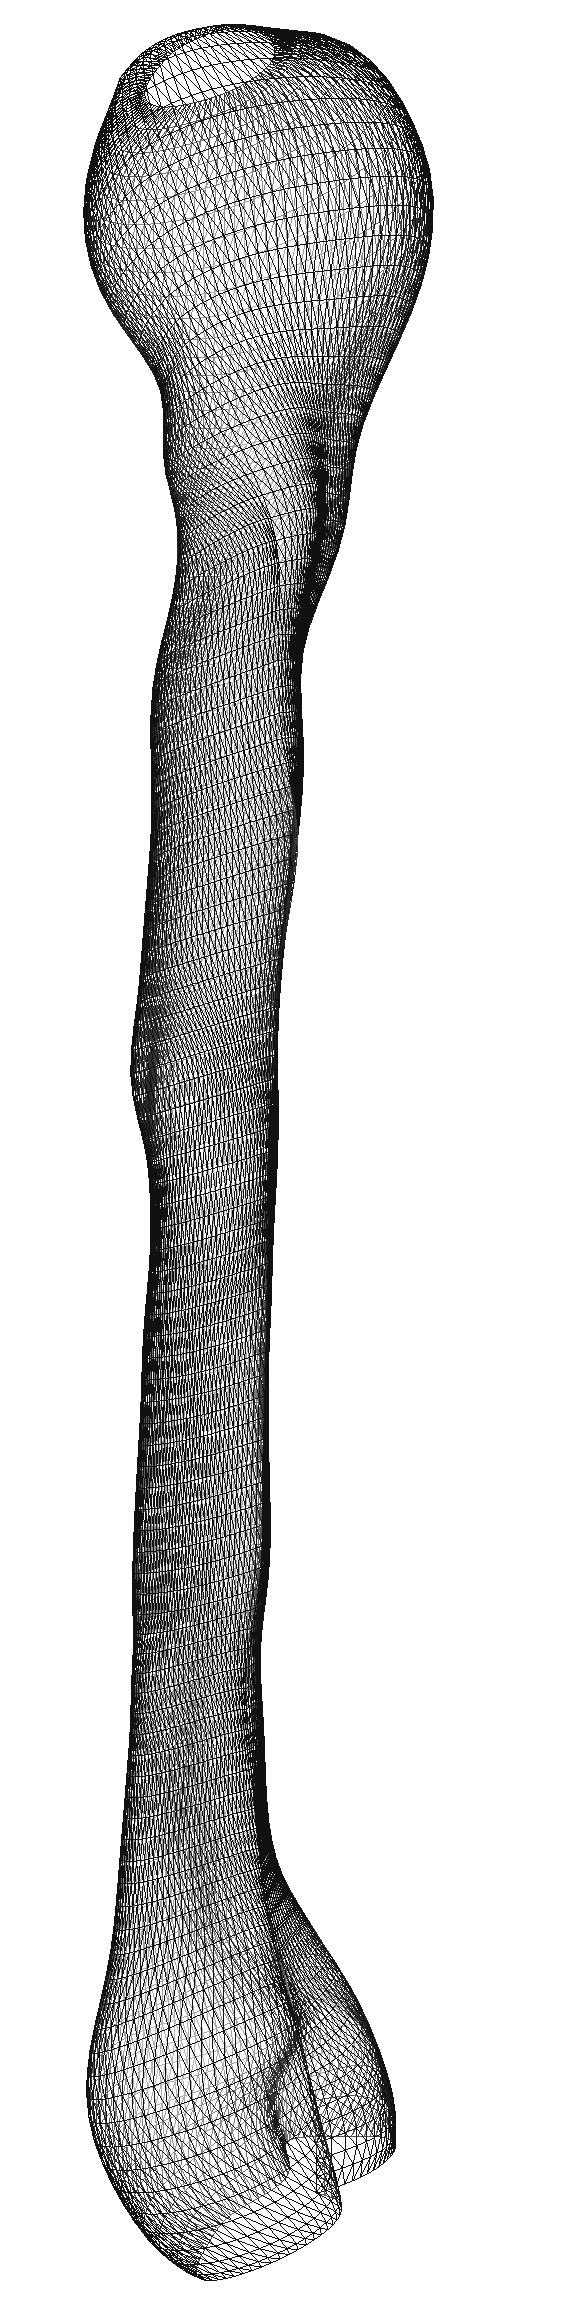
\includegraphics[height=6cm]{images/fiber_creation/extraction_humerus00.png}%
    \caption{Surface of the humerus}%
    \label{fig:extraction_result_humerus}%
  \end{subfigure}    
  \caption{Resulting surfaces of biceps and humerus bone obtained by the automatic surface extraction algorithm.}%
  \label{fig:extraction_result}%
\end{figure}%

The runtime for the algorithm is \SI{121}{\minute} on a AMD Ryzen 5 1600 processor with 6 cores, 3.2 GHz and \SI{16}{\giga\byte} RAM, of which a maximum of \SI{2}{\giga\byte} was used at maximum. Because processing of the images can be done in parallel, the runtime can be reduced to approximately half (\SI{62}{\minute}) using 2 threads and to a quarter (\SI{30}{\minute}) using 6 threads.

The advantage of the presented algorithm is that the outcome solely depends on the imaging data and, thus, no modeling error by manual approximation of the geometry occurs. For example, the obtained surfaces of biceps and humerus geometrically fit perfectly into each other. Intermediate steps are stored as black and white images. By editing these between the steps of the algorithm, manual tweaking is possible and could lead to increased quality of the results.

A disadvantage is that it relies on color information in the imaging data to differentiate between muscle and other tissue. Because the involved tissue has similar colors, these differences are often small. Furthermore, the color ranges need to be determined experimentally. Therefore, the algorithm is not very robust with respect to image noise and needs adjustments when it should be used to extract other muscles. Expert knowledge about the location and shape of human muscles cannot be used easily to improve the results of the algorithm.

A different approach is to manually segment the imaging data and construct surfaces with the help of a tool. This approach is described in the following section.

\subsection{Manually guided surface extraction}\label{sec:surf_extr}

The manually guided segmentation is done using the \emph{MAP client} of the Musculoskeletal Altas Project (MAP) \cite{mapclient}. This application allows to create and execute a workflow to achieve data processing and simulation tasks. In a graphical window, the user can place and connect various workflow steps. When executing the workflow, each step shows a dialog where the required configuration can be entered or the operations can be performed on a visual presentation of the data at this workflow stage. 

Possible workflow steps include source and sink operations such as reading image data and writing meshes. Imaging data such as the 2D images from the Visual Human Male can be visualized in a 3D representation. The user can place points in the 3D space and try to match borders of the muscles and structures to extract from the data.
Further workflow steps allow to create meshes of predefined geometrical shapes, such as cubes and cylinders and merge them into a common mesh. These meshes can be fitted to point clouds of user defined points. This is done by a least squares approach minizing the distances between user created points and the mesh surface.

The MAP client has a plugin architecture and allows to create new workflow steps. It includes features from OpenCMISS, especially data processing formats and tools from OpenCMISS Zinc. Meshes can be created with 3D cubic Hermite elements that allow a high geometric modelling flexibility with a low number of nodes. Such meshes are stored in the OpenCMISS file format of \code{exnode} and \code{exelem} files.

As a result, meshes of individual muscles or the whole human organism can be created. \Cref{fig:vhp_geometry} shows meshes that were create from the cryosectioning data of the Visible Human Male. In \cref{fig:vhp_total} almost the whole body has been extracted. In \cref{fig:vhp_detail}, the mesh consisting of cubic Hermite elements is visualized. A relatively coarse mesh width suffices to model a smooth surface of the body. When exported in the exfiles format from the MAP client, the data can be visualized, e.g., using \emph{cmgui}, the visualization tool of OpenCMISS Zinc.

\begin{figure}%
  \centering%  
  \begin{subfigure}[t]{0.48\textwidth}%
    \centering%
    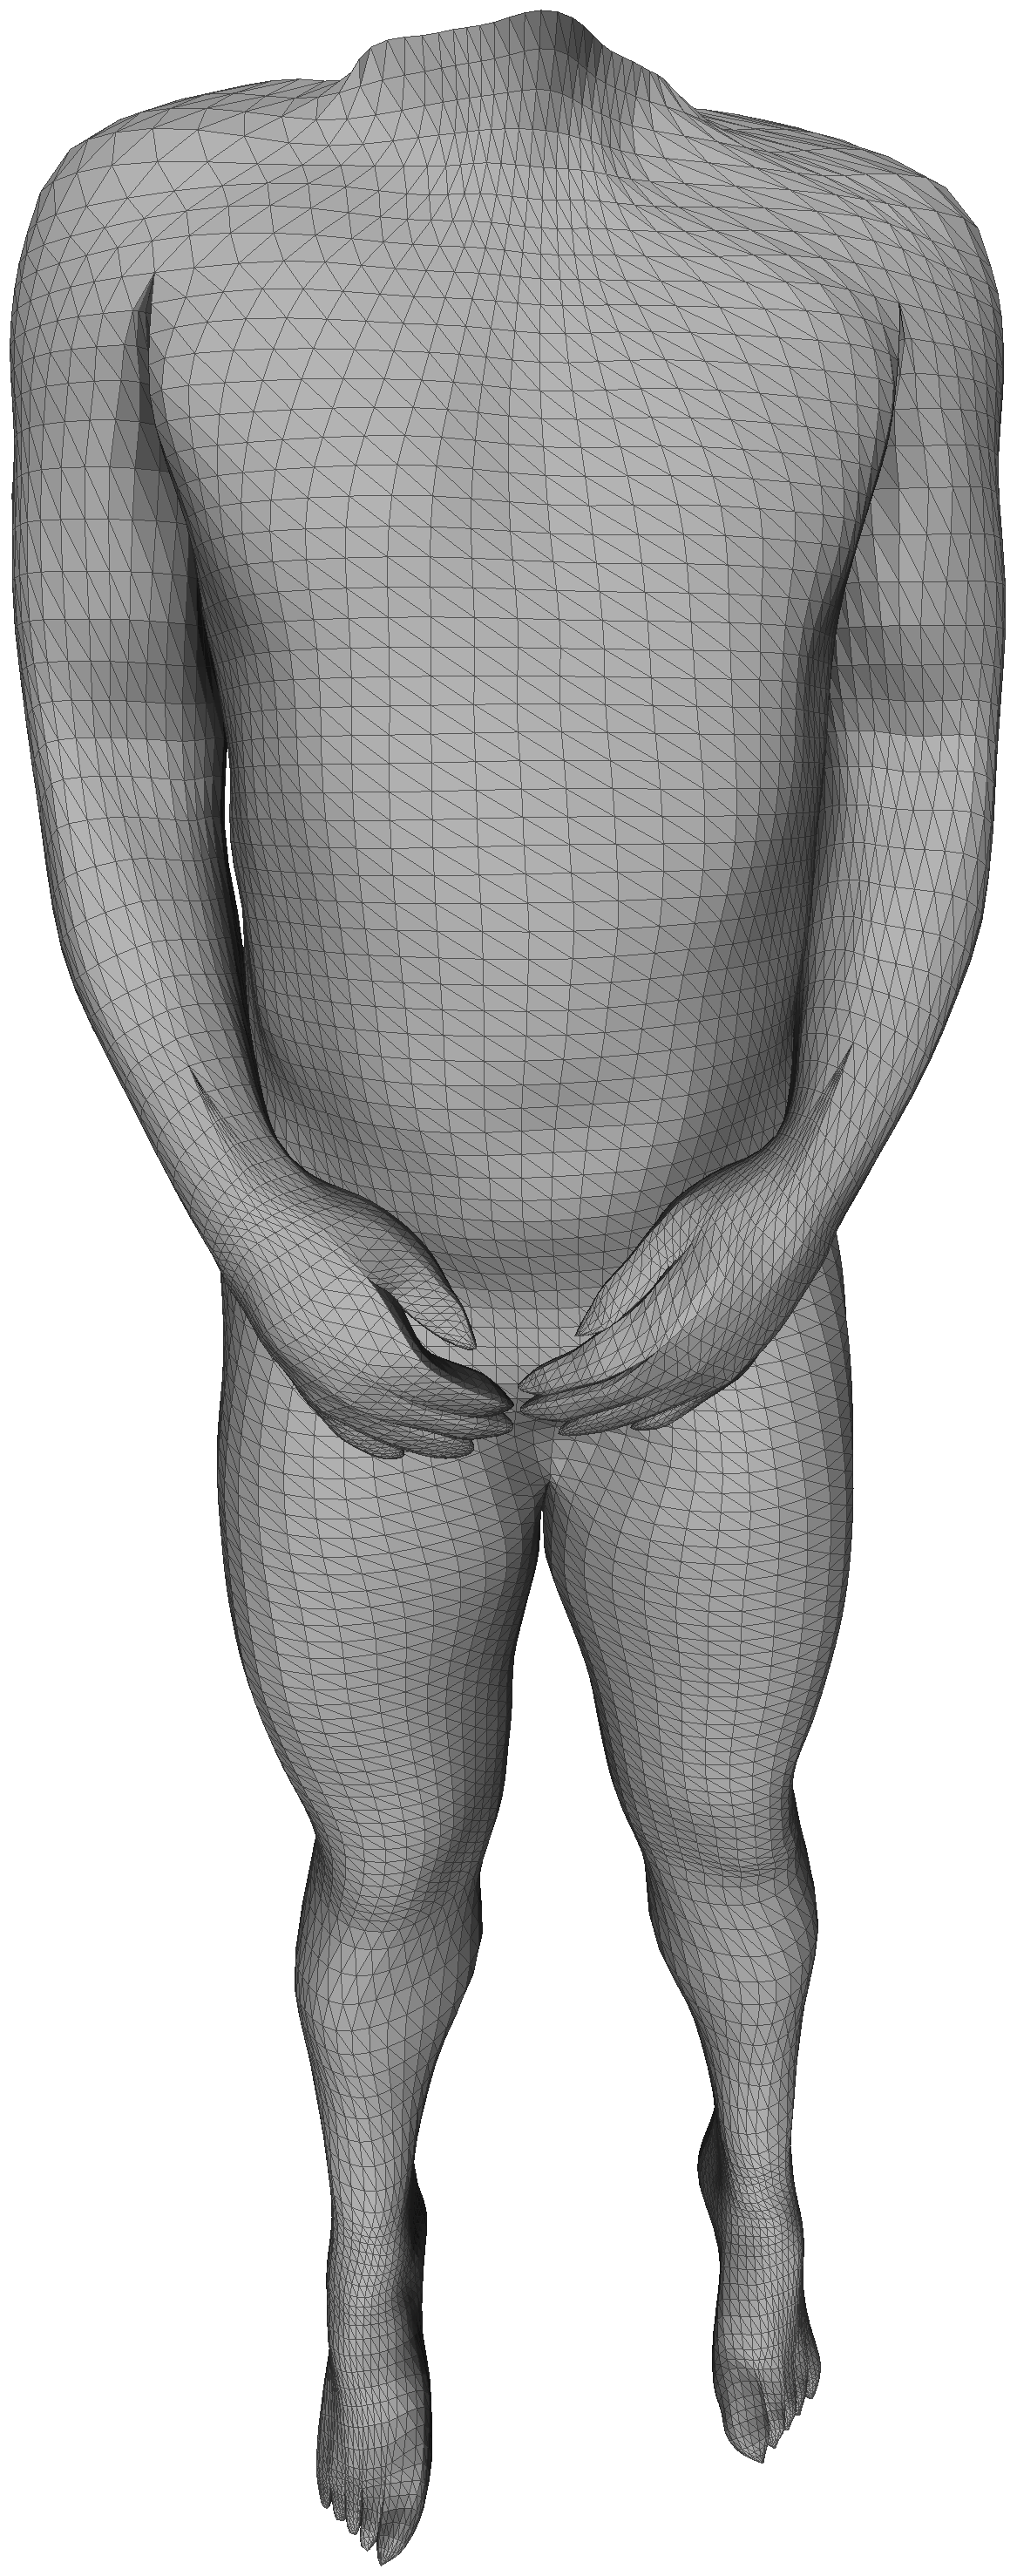
\includegraphics[height=10cm]{images/fiber_creation/skin00.png}%
    \caption{Mesh of the trunk and limbs, surface has been triangulated for visualization.}%
    \label{fig:vhp_total}%
  \end{subfigure}
  \quad
  \begin{subfigure}[t]{0.48\textwidth}%
    \centering%
    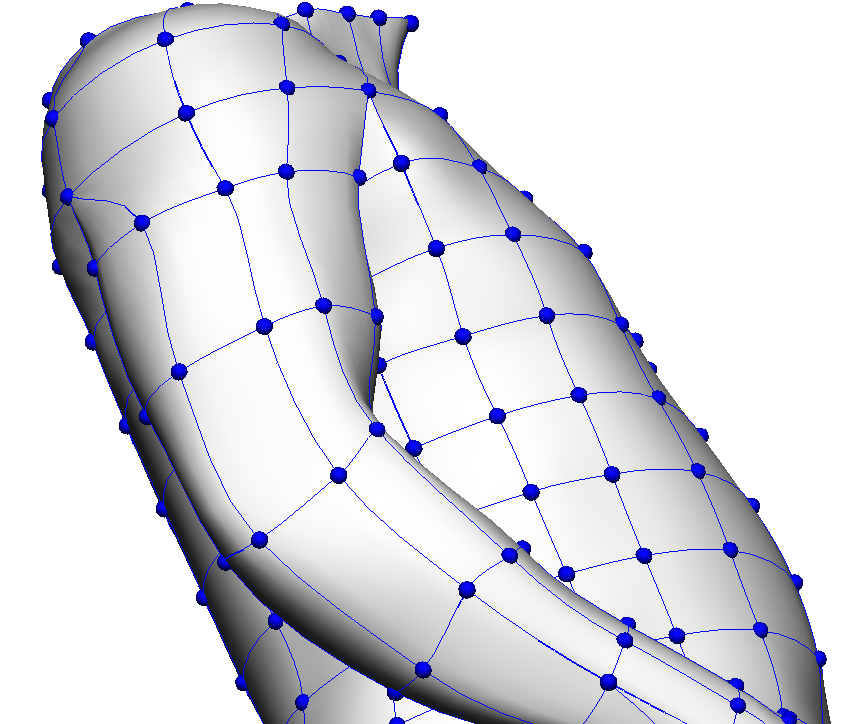
\includegraphics[height=7cm]{images/fiber_creation/elements4.png}%
    \caption{Detail view of part of the right upper arm and the trunk with blue nodes and contours of a mesh with cubic Hermite elements.}%
    \label{fig:vhp_detail}%
  \end{subfigure} 
  \caption{Mesh of the Visible Human Male from the Visible Human Project.}%
  \label{fig:vhp_geometry}% 
\end{figure}%

The mesh width of the meshes obtained using the MAP client was chosen such that the surface fitting yielded good results. The meshes are not necessarily ready for use in a simulation, especially if a  high mesh resolution is desired. 
Apart from the mesh width also the type of elements can be different than what is needed for a Finite Element simulation. Our goal is to obtain meshes with linear or quadratic Lagrange elements with configurable mesh widths for the specified upper arm muscles, such as the biceps brachii.

Therefore, the next step of the workflow, as visualized by the right branch of \cref{fig:scheme_preprocessing}, is to transform the volume mesh into a surface mesh which then can be used as basis for further meshing. This is visualized with the example of the biceps muscle in \cref{fig:biceps_processing}. The basis is the Hermite mesh shown in the left-most image.

\begin{figure}%
  \centering%
  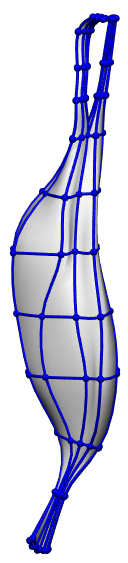
\includegraphics[height=10cm]{images/fiber_creation/exfile.png}\quad%
  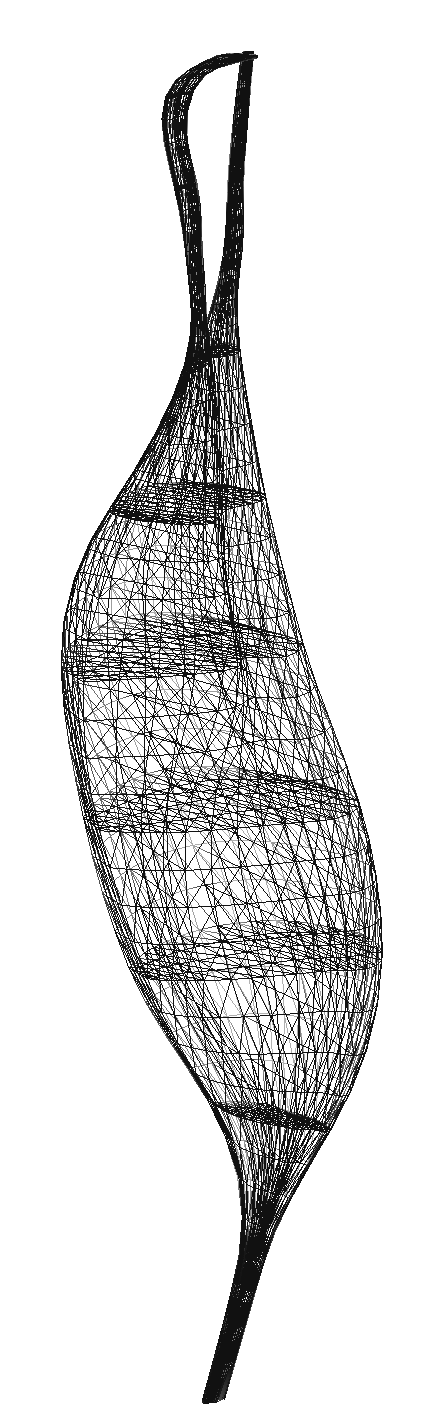
\includegraphics[height=10cm]{images/fiber_creation/biceps23.png}%
  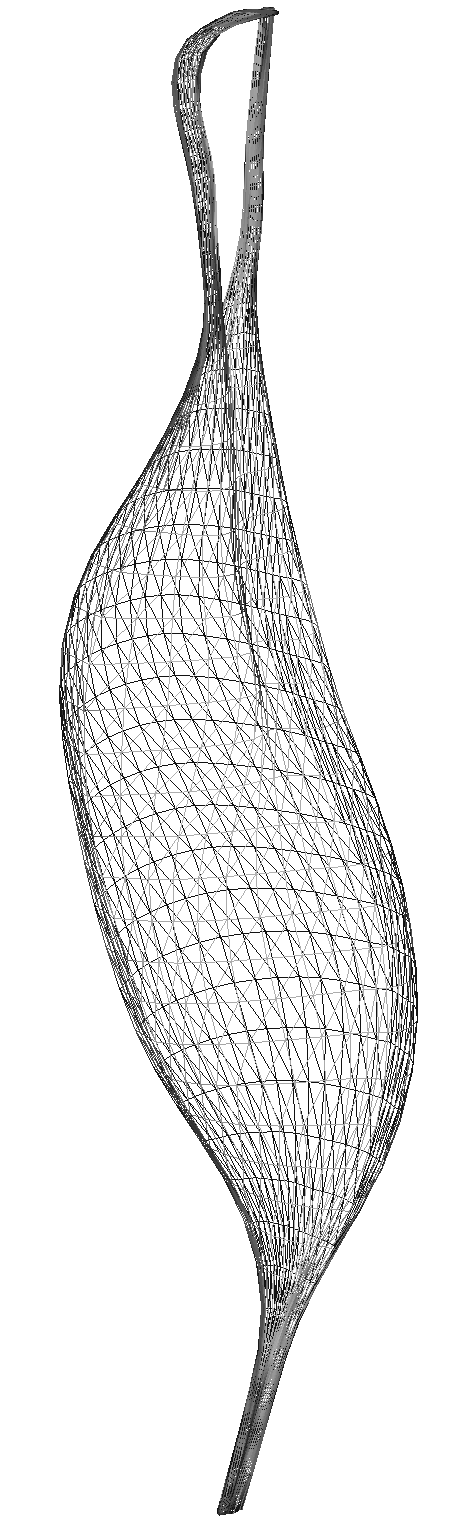
\includegraphics[height=10cm]{images/fiber_creation/biceps22.png}%
  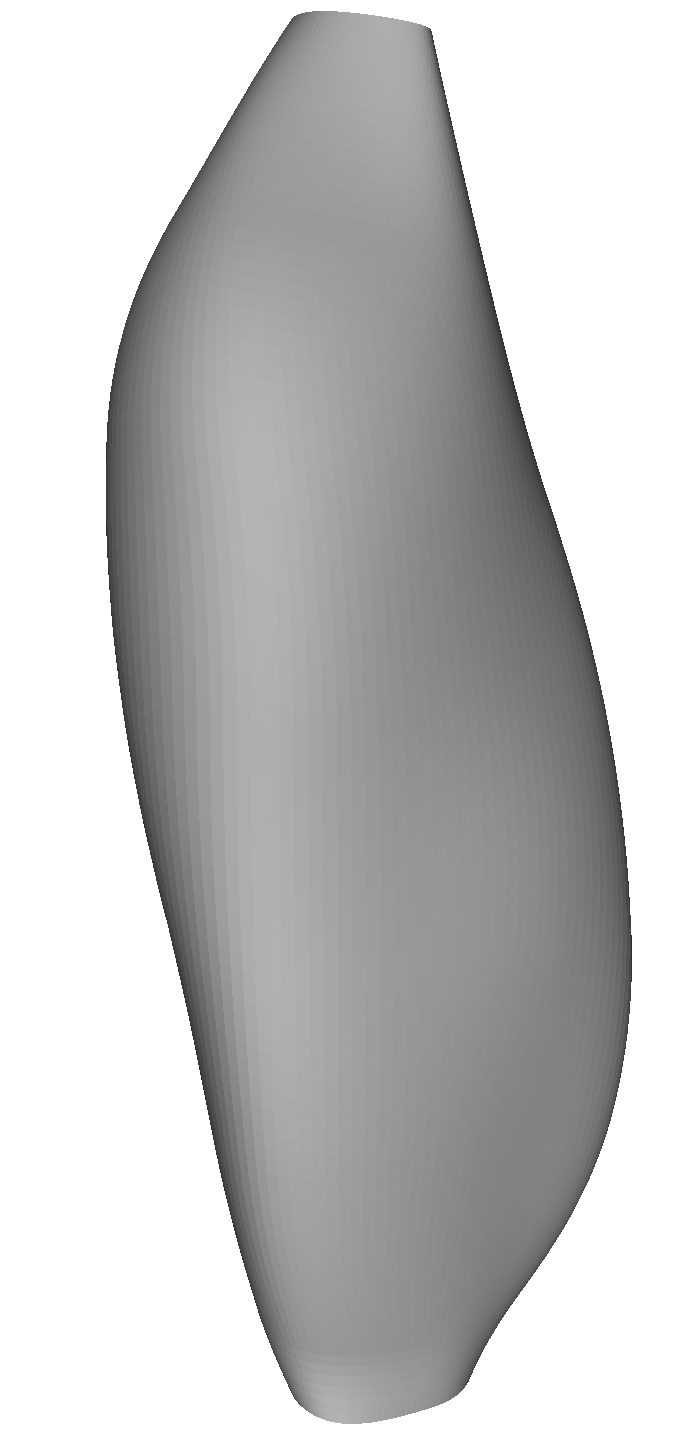
\includegraphics[height=10cm,trim=-2cm 0 0 -2cm, clip]{images/fiber_creation/splines00.png}%
  \caption{Processing the geometry of the biceps brachii muscle. From left to right: mesh with cubic Hermite elements, STL mesh with inside triangles, STL surface mesh where triangles lying inside have been removed, Spline surface of the muscle belly.}%
  \label{fig:biceps_processing}%
\end{figure}%

The Hermite elements can be triangulated and stored as an STL file using the tool \code{cmgui}. This process triangulates the non-planar faces of all Hermite elements. This leads to a dataset with triangles on the surface and in the inside of the volume, as can be seen in the second image of \cref{fig:biceps_processing}. At this stage, the use of the MAP and OpenCMISS related tools is finished and further processing steps are performed using tools from opendihu that we developed on our own.

A Python script removes the triangles in the inside of the volume. The detection whether a triangle is inside the volume is done by casting four rays from the center of gravity of the triangle and determining if the rays intersect any other triangles. The rays have directions $(x,y,z) = (\pm1,\pm1,\frac13)$, where the $z$ axis is oriented along the muscle and the $x$ and $y$ are oriented in radial direction. The ray-triangle intersection is done using the fast Möller-Trumbore algorithm \cite{ray-triangle}. For every ray, all triangles are checked.
Only if all four rays intersect at least one more triangle, the starting triangle is considered to be inside the volume and subsequently removed from the dataset. 

This algorithm has a quadratic time complexity $\O(n^2)$ in the number of triangles $n$. It could be improved by organizing the triangles in a spatially adaptive data structure, such as an octree. Since this preprocessing step has to be performed only once for a given geometry the runtime is not a concern and there is no need for such optimization.

The result of this operation is a triangulated surface, shown in the third image of \cref{fig:scheme_preprocessing}. The next step is to create a Spline surface of the muscle belly, as shown in the right-most image of \cref{fig:scheme_preprocessing}. This is described in the next section.

\subsection{Fitting a Spline surface}\label{sec:nurbs}
The surface representation of the muscle could be obtain from either the left or the right branch of the preprocessing workflow in \cref{fig:scheme_preprocessing}. The surface is given by a point cloud or a number of triangles. To remedy eventual outliers or unphysiological sharp edges from the segmentation, a Spline surface is fitted to the data. This leads to a smooth surface representation and later to a better conditioned Finite Element mesh in the simulation. However, this step is optional. It is also possible to use the surface triangulation from previous section \ref{sec:surf_extr} for the meshing algorithm in the next section \ref{sec:ser_alg_meshes}.

Nonuniform rational B-Splines (NURBS) are used for the surface. A NURBS surface is a generalization of a B-Spline surface. From a modeling point of view, B-spline surfaces have three advantages. First, the B-spline surface can be constructed with given smoothness properties.  Second, the definition of a particular B-spline surface builds on geometric information, which simplifies their creation. More specifically a control polygon mesh in the 3D space is defined. Its convex hull is guaranteed to contain the surface. Third, the geometric parameters of a B-spline surface have only local impacts on the shape of the surface. This allows a B-spline surface of a fixed, low polynomical degree to approximate point clouds with any number of points without loosing approximation quality.

A limitation of B-spline surfaces is that circular and spherical shapes cannot be represented. This limitation is overcome by NURBS surfaces. NURBS surfaces are defined as the perspective projection into 3D space of a B-spline surface in 4D space.

The mathematical description is given in this section, following the notation of \cite{piegl2012nurbs}. The building blocks are the B-spline basis functions of polynomial degree $p$. Given a knot vector 
%
\begin{align*}
  \Xi = (\xi_1, \xi_2, \dots, \xi_k), \quad \text{with } a=\xi_1 \leq \xi_2 \leq \cdots \leq \xi_k = b,
\end{align*}
%
the $i$th B-spline basis function $N_{i,n}$ of degree $n$ is defined recursively starting with the piecewise constant function $N_{i,0}$ for $n=0$,
%
\begin{align*}
  N_{i,0}(\xi) = \begin{cases} 
    1 \, &\xi_i \leq \xi < \xi_{i+1},\\[2mm]
    0 &\text{else},
  \end{cases}
\end{align*}
and using the following relation to define the functions of higher degree, $n > 0$,
\begin{align*}
  N_{i,n}(\xi) = \dfrac{\xi - \xi_i}{\xi_{i+n} - \xi_i} N_{i,n-1}(\xi) + \dfrac{\xi_{i+n+1} - \xi}{\xi_{i+n+1} - \xi_{i+1}} N_{i+1,n-1}(\xi), \quad i > 0.
\end{align*}
Because neighbouring entries in the knot vector can be equal, the fraction $0/0$ can occur. In this case, $0/0 := 0$ is defined.

A B-spline curve $\bfC \in \R^d$ of polynomial degree $p$ is defined as
%
\begin{align*}
  \bfC(u) = \s{i=1}{l}N_{i,p}(u)\,\bfP_i, \quad u \in [a,b].
\end{align*}
%
The coefficients $\bfP_i \in \R^d, i=1, \dots, l$ to the basis functions $N_{i,p}$ are called \emph{control points} and define the control polygon. The number $l$ of basis functions and control points is determined from the number of knots $k$ in an open knot vector and the polynomial degree $p$ as $l = k-p-1$.

The number of equal entries in series in the knot vector is the \emph{multiplicity} of the respective knot value. Usually \emph{open} knot vectors $\Xi$ are used where the first and the last knot occur with a multiplicity of $p+1$.
This make the first and last points of the B-spline curve coincide with the control polygon, $\bfC(a) = \bfP_1$ and $\bfC(b) = \bfP_l$.

The multiplicities of the knots in the knot vector encode information about the smoothness of the B-spline curve. If the knot value $\hat{\xi}$ has a multiplicity of $m$, the B-spline curve will be $p-m$ times continuously differentiable at $\C(\hat{\xi})$.
% This can be seen from the fact that there exist $m$ basis functions with a support that begins at $\hat{\xi}$.

An exemplary B-spline curve is shown in \cref{fig:bspline_curve}. It uses a \emph{non-uniform} knot vector for polynomial degree $p=3$, where the differences between neighbouring knot values $\xi_{i+m} - \xi_i$ vary. The effect of different multiplicities can be seen. $m=p=3$ places the knot on the respective control point, as for $\xi=49$ in the example. $m=p-1=2$ places the knot on the control polygon, as in the example at $\xi=10$. A lower multiplicity $m < p-1$ does not yield to a higher smoothness and in turn does not force the curve on the control polygon. It can also be seen that the B-spline curve stays inside the convex hull of the control polygon which is a property of all B-spline curves \cite{piegl2012nurbs}.
%
\begin{figure}%
  \centering%
  \def\svgwidth{8cm}%
  \input{images/fiber_creation/bspline_curve.pdf_tex}%
  \caption{Exemplary B-spline curve (red) of degree $p=3$ for the knot vector $\Xi = (0,0,0,0,7,10,10,49,49,49,50,50,50,50)$, control points (blue) and control polygon (black).
  Positions of the curve $\bfC(\xi_i)$ at the knots $\xi_i$ are indicated by the red squares and the knot value $\xi$ and its multiplicity $m$ is given. The effect of moving one control point is shown in green.}%
  \label{fig:bspline_curve}%
\end{figure}%
%
The effect of moving one of the 10 control points is visualized with green color in the \cref{fig:bspline_curve}.
The B-spline basis function $N_{i,p}$ has a local support of $S=(\xi_i,\xi_{i+p+1})$. Consequently, only the corresponding part of the curve, $\bfC(\xi)$ for $\xi \in S$ changes.

A B-spline surface is given as tensor product of two B-spline curves:
\begin{equation}\label{eq:bspline_surface}
  \begin{array}{lll}
    \bfS(u,v) = \s{i=1}{l^{(1)}}\s{j=1}{l^{(2)}} N^{(1)}_{i,p^{(1)}}(u)\,N^{(2)}_{j,p^{(2)}}(v)\, \bfP_{i,j},
  \end{array}
\end{equation}
with two polynomial degrees $p^{(1)},p^{(2)}$, ansatz functions $N^{(1)}, N^{(2)}$, numbers of ansatz functions $l^{(1)}, l^{(2)}$ and corresponding knot vectors.

For NURBS, B-spline curves and surfaces are formulated using \emph{homogeneous coordinates}. Every point in Cartesian coordinates $(x,y,z) \in \R^3$ has a set of homogeneous coordinates $(\tilde{x},\tilde{y},\tilde{z},w)=(x\,w,y\,w,z\,w,w)$. Thus, the Cartesian coordinates can be obtain by the \emph{perspective division}, i.e. dividing all but the last coordinate by the weight $w$.

A NURBS surface is given by the same definition as the B-spline surface in \cref{eq:bspline_surface} except that the control points $\bfP_{i,j} \in \R^3$ are enriched with scalar weights $w_{i,j}$ and, thus, replaced by $(\bfP_{i,j}, w_{i,j}) \in \R^4$. The resulting surface $\bfS$ is given in homogenous coordinates. Executing the perspective division yields the form:
%
\begin{align*}
  &\bfT(u,v) = \s{i=1}{l^{(1)}}\s{j=1}{l^{(2)}} R_{i,j}(u,v) \,\bfP_{i,j},\\[4mm]
  &\text{with } R_{i,j}(u,v) = \dfrac{N_{i,p^{(1)}}(u)\,N_{j,p^{(2)}}(v)\,w_{i,j}}{\s{r=1}{l^{(1)}}\s{s=1}{l^{(2)}} N_{r,p^{(1)}}(u)\,N_{s,p^{(2)}}(v)\,w_{r,s}}.
\end{align*}
The new rational basis functions $R_{i,j}$ and the possibly non-uniform knot vectors give rise to the name non-uniform rational B-spline surface.

In order to find a NURBS surface for the given triangulated surface of a muscle, at first, the part of the geometry corresponding to the tendons is removed) such that the resulting triangles model only the muscle belly. The belly has a length of \SI{12.8}{\mm}.

Then, twelve cross sections are extracted from the surface triangles. The result are twelve horizontal circumference rings. On each ring 9 equidistant points are sampled. The first point is appended after the last point in every ring, such that in total we obtain a grid of $10 \times 12$ points. The least squares surface approximation algorithm by \cite{piegl2012nurbs} is used to fit a NURBS surface to the points. The implementation of the algorithm is given by the NURBS-Python (geomdl) library. Polynomial degrees of $p^{(1)} = 3$ and $p^{(2)}=2$ are used where the first dimension corresponds to the cross-sectional direction of the muscle. The knot multiplicity is chosen as $m=1$ for both coordinate directions to obtain a two times respective one times continuously differentiable surface in $u$ and $v$ direction. The resulting NURBS surface and the control polygon is visualized in \cref{fig:biceps_splines_control_points}. Note that the control polygon is different from the grid of points against which the surface is fitted.
%
\begin{figure}%
  \centering%
  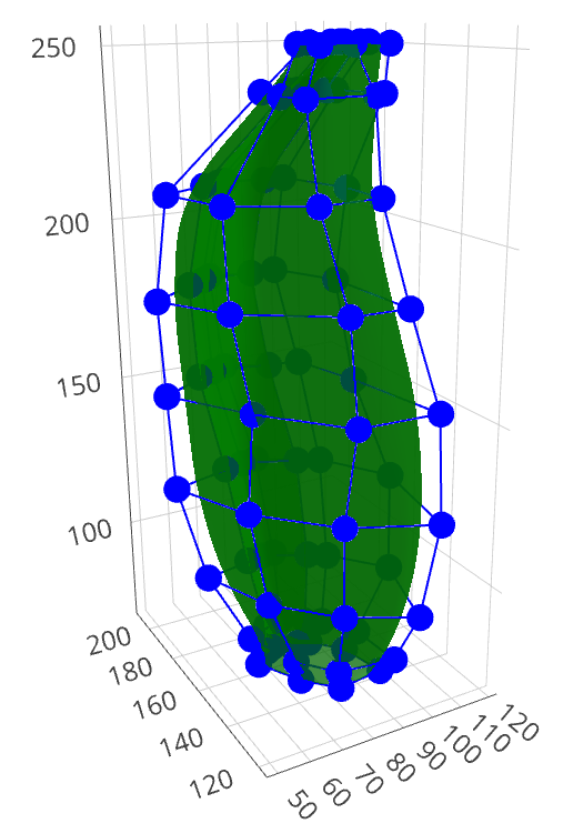
\includegraphics[width=0.35\textwidth]{images/fiber_creation/splines01.png}%
  \caption{Fitted NURBS surface of the biceps muscle (green) and the control polygon (blue).}%
  \label{fig:biceps_splines_control_points}%
\end{figure}%
%
\Cref{fig:biceps_splines_wrong} shows the result of this approach. It can be seen the surface is non-differentiable and has a kink at the seam line where the first and last points of each ring meet. The reason is that the surface fitting algorithm does not pose any conditions on the tangents at the edges of the fitted NURBS surface. Since no implementation of a fitting algorithm specifically for a tubular NURBS surface is available, the point grid is modified. The series of 9 equidistant points on each ring is replicated twice and the first point is again added as the last point. This leads to a grid of $(3\cdot 9+1) = 28 \times 12$ points which wraps around the muscle volume three times. The fitting algorithm is executed on this grid. The resulting NURBS surface also wraps around the muscle three times with the two ends being again not properly fitting to each other. From these three wraps, the middle one is extracted. This corresponds to restricting the NURBS surface $\bfT(u,v)$ from $(u,v) \in [0,1]^2$ to $(u,v) \in [0.4,0.733]\times [0.1]$.

The result is depicted in \cref{fig:biceps_splines_seam} and it can be seen that the tangents now match very well between the two sides of the NURBS surface. Furthermore, the comparison with the inital approach in \cref{fig:biceps_splines_wrong} shows that an artifical bulge at the top of the muscle in the perspective of the visualization is removed. The overall shape of the muscle now looks smoother and more natural. Also in comparison with the result of the automatic algorithm in \cref{fig:extraction_result_biceps}, the results of this approach are smoother.

The generated tubular surface has two holes at the top and bottom which prevent it from being an enclosing surface to the muscle belly volume. The borders of these holes each lie in a plane and, thus, the missing surface is treated as being planar when the 3D meshes are created.
%
\begin{figure}%
  \centering%
  \begin{subfigure}[t]{0.48\textwidth}%
    \centering%
    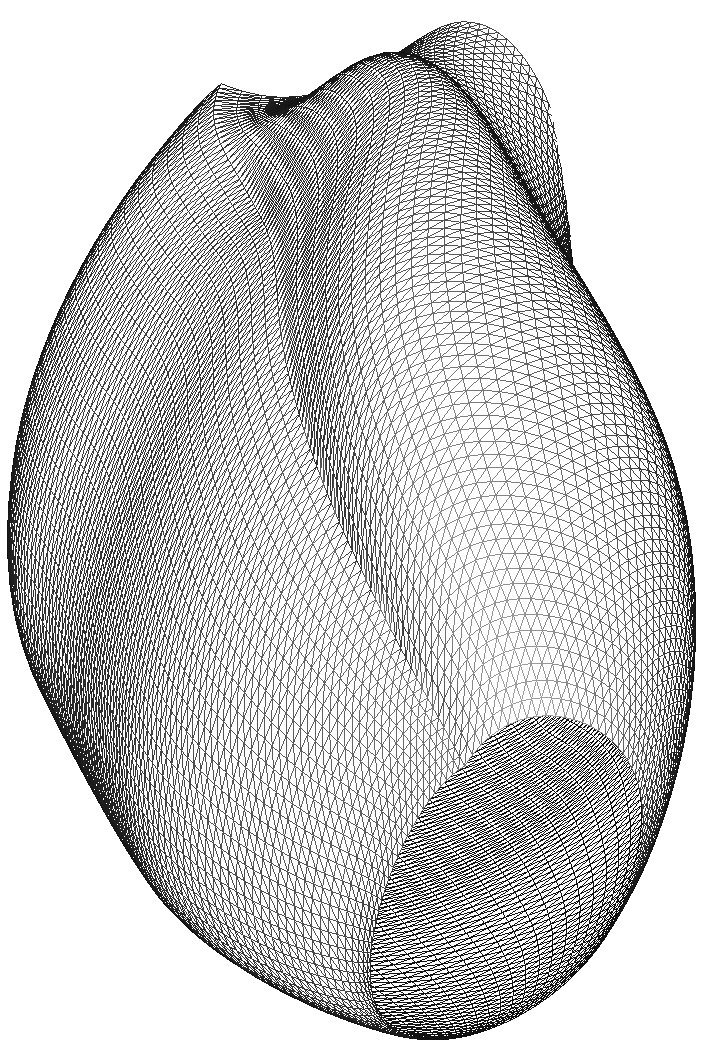
\includegraphics[height=8cm]{images/fiber_creation/splines_wrong00.png}%
    \caption{First approach with $10 \times 12$ points. The kink at the seam line along the muscle is clearly visible.}%
    \label{fig:biceps_splines_wrong}%
  \end{subfigure}
  \quad
  \begin{subfigure}[t]{0.48\textwidth}%
    \centering%
    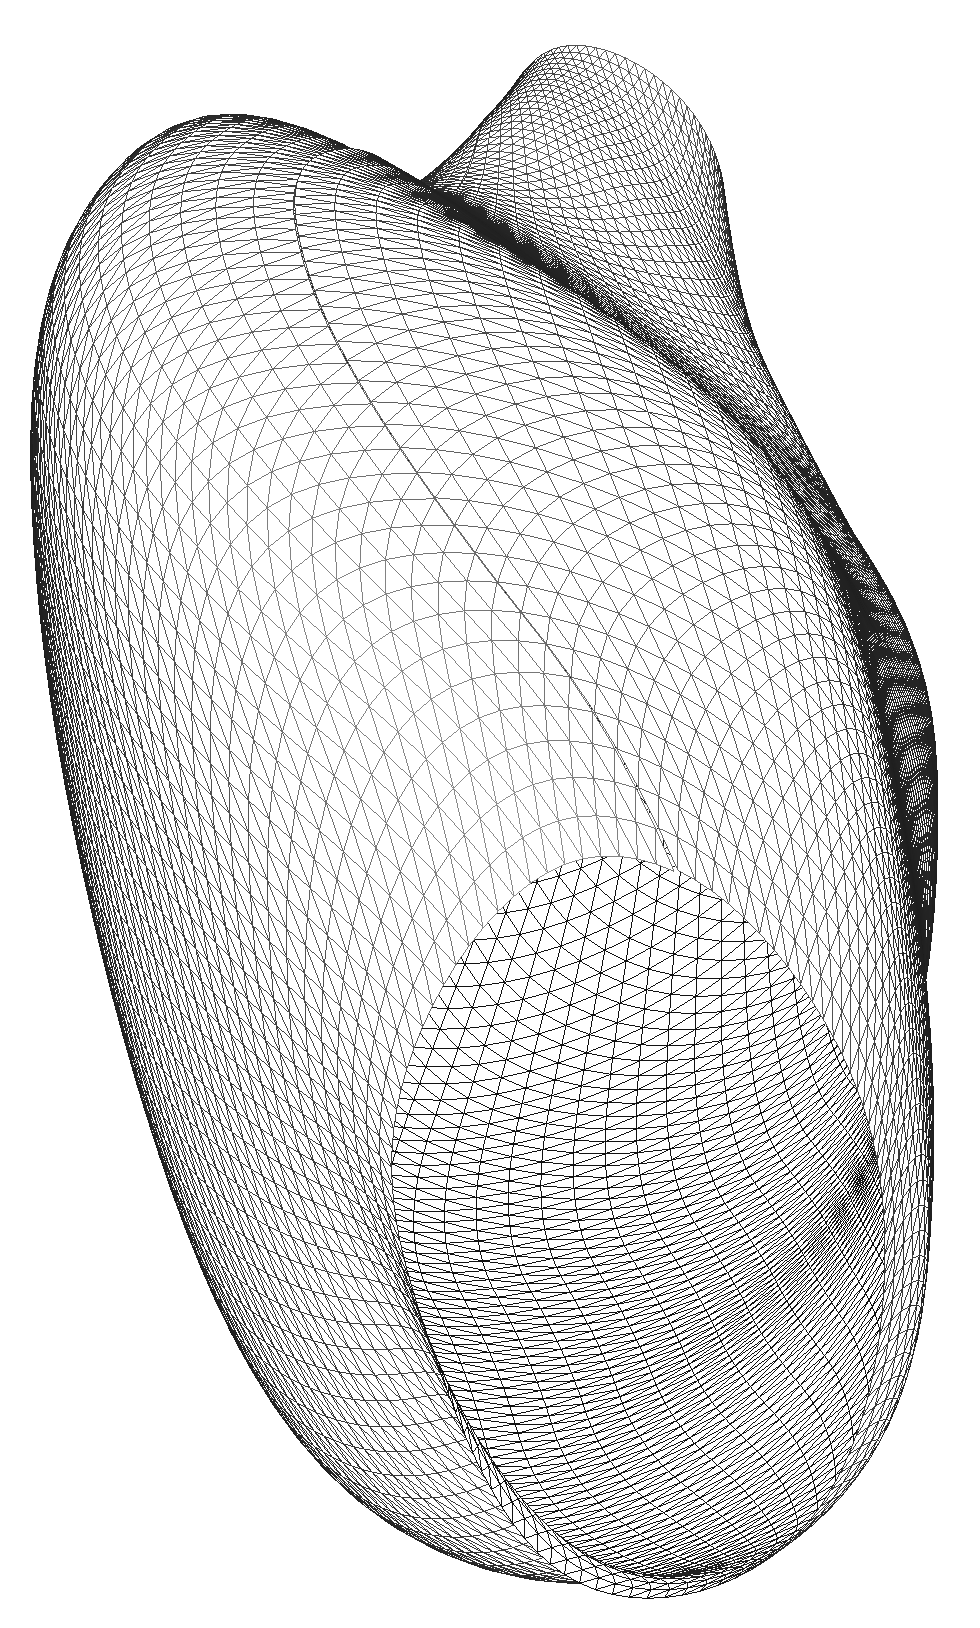
\includegraphics[height=8cm]{images/fiber_creation/splines_seam00.png}%
    \caption{Second, improved approach with $28 \times 12$ points. It can be seen that the tangent at the seam line matches very well.}%
    \label{fig:biceps_splines_seam}%
  \end{subfigure}
  \caption{Fitted NURBS surface of the biceps muscle, triangulated for visualization purposes.}%
  \label{fig:biceps_splines}%
\end{figure}%
%
\section{Serial Algorithm to Create Muscle and Fiber Meshes}\label{sec:ser_alg_meshes}
Next, a 3D mesh for the muscle volume and 1D meshes for muscle fibers need to be generated from the surface representation described in the last sections. In this section, first an algorithm for the 3D mesh is described. Then, a second algorithm that reuses results from the first algorithm is presented which generated one dimensional meshes for muscle fibers. Both algorithms are executed in serial. A derived algorithm that can run in parallel and, thus, on a distributed memory hardware can handle larger datasets is given in the next section, \cref{sec:parallel_algorithm}.

The serial algorithm for generation of the 3D mesh is presented in \cref{alg:serial_algorithm_1} and the steps visualized in \cref{alg:serial_algorithm_1}. Input is the set of triangles at the tubular surface of the muscle. The tubular surface is oriented along the $z$ axis. In the following descriptions the muscle in considered to be oriented upright such that $z$ axis points in vertical direction towards the top. The borders at bottom and top have a constant $z$ coordinate.
%
\begin{algorithm}
  \begin{algorithmic}[1]%
    \Procedure{Create\_3D\_mesh}{}
    \Require triangulated tubular surface
    \Ensure structured 3D volume mesh
    \Statex
    \State Slice geometry           \label{alg:1.1}
    \State Triangulate 2D slices      \label{alg:1.2}
    \State Compute harmonic maps $u, v$      \label{alg:1.3}
    \State Construct regular grid in parameter space and map to slices            \label{alg:1.4}
    \State Form 3D quadrilateral elements between the 2D slices’ meshes   \label{alg:1.5}
    \EndProcedure
  \end{algorithmic}%
  \caption{Serial algorithm}%
  \label{alg:serial_algorithm_1}%
\end{algorithm}%

\subsection{Slicing of the geometry}
The first step in line \algref{alg:serial_algorithm_1}{alg:1.1} states to slice the geometry. This means that horizontal \say{slices} of the cross-sectional area are extracted from the surface mesh. First, the muscle is divided into equidistant positions $z_i, i=1,\dots,n$ along the $z$-axis where the slices are to be extracted. As can be seen in \cref{fig:serial_alg_0}, $n=13$ $z$ coordinates are selected. Next, for every position $z_i$, all surface triangles $T_j$ that intersect the plane $Z_i = \{\bfp=(x,y,z) | z=z_i$\} are considered and the intersection lines $P = T_j \cap Z_i$ are computed. The method of computing plane-triangle intersection is described in the following.

Given is a triangle $T$ with points $\bfp^{1},\bfp^2,\bfp^3 ∈ \R^3$ and a value $\hat{z}$, the wanted result is the set of points $P = T ∩ \{\bfp = (\bfp_x,\bfp_y,\bfp_z) \mid \bfp_z=\hat{z}\}$ which corresponds to a line segment $\overline{\bfp^a\bfp^b}$. 

We describe the points in the triangle by two barycentric coordinates $\xi_1$ and $\xi_2$ as
\begin{equation}\label{eq:barycentric_triangle}
  \begin{array}{lll}
    \bfp(ξ_1,ξ_2) = (1-ξ_1-ξ_2)\,\bfp^{1} + \xi_1\,\bfp^{2} + \xi_2\,\bfp^{3},  \\[4mm]
    \text{with }\xi_1+\xi_2 \leq 1, \quad 0 \leq \xi_1,\xi_2 \leq 1.
  \end{array}
\end{equation}
By letting $\bfp_z(ξ_1,ξ_2) = \hat{z}$ we calculate the equation for the line segment $\overline{\bfp^a\bfp^b}$ in barycentric coordinates to be
\begin{equation*}
  \begin{array}{lll}
    ξ_1 = m\cdot ξ_2 + c,\quad
    m = -\dfrac{\bfp_z^{3} - \bfp_z^{1}}{\bfp_z^{2} - \bfp_z^{1}}, \quad c = \dfrac{\hat{z} - \bfp_z^{1}}{\bfp_z^{2} - \bfp_z^{1}}, \quad \bfp_z^2 \neq \bfp_z^1.
  \end{array}
\end{equation*}
For $\bfp_z^1 = \bfp_z^2 \neq \bfp_z^3$ we swap $\bfp_z^2$ and $\bfp_z^3$.

%
%  # x(xi1,xi2) = (1-xi1-xi2)*x^{1} + xi1*x^{2} + xi2*x^{3},  xi1+xi2 <= 1, 0 <= xi1,xi2 <= 1
%  # x_3(xi1,xi2) = z_value  =>  (1-xi1-xi2)*x^{1} + xi1*x^{2} + xi2*x^{3} = z_value
%  #                         =>  xi1*(x^{2} - x^{1})  +  xi2*(x^{3} - x^{1})  =  z_value - x^{1}
%  #                         =>  xi2 = ((z_value - x^{1}) - xi1*(x^{2} - x^{1})) / (x^{3} - x^{1})
%  #                         =>  xi2 = (z_value - x^{1})/(x^{3} - x^{1}) - xi1 * (x^{2} - x^{1})/(x^{3} - x^{1})
%  #                         =>  xi1 = (z_value - x^{1}) / (x^{2} - x^{1})  - xi2 * (x^{3} - x^{1}) / (x^{2} - %x^{1}) 
We consider the three sides $\overline{\bfp^1\bfp^2}, \overline{\bfp^2\bfp^3}$ and $\overline{\bfp^3\bfp^1}$ of the triangles and check which of them is intersected by the $z=\hat{z}$ plane.
\begin{enumerate}
\item On the triangle side $\overline{\bfp^1\bfp^3}$ we have the condition $ξ_2 = 0$ and the side intersects the plane 
at $\bfp(0,-c/m)$ 
iff $0 \leq c \leq 1$. 
\item On the triangle side $\overline{\bfp^1\bfp^2}$, the condition $ξ_1 = 0$ holds and the side intersects the plane 
at $\bfp(c,0)$ 
iff $m\neq 0 \wedge 0 \leq -c/m \leq 1$. 
\item The third triangle side $\overline{\bfp^2\bfp^3}$ is intersected for $ξ_1=(c+m) / (1+m)$
at $\bfp(ξ_1,1-ξ_1)$ 
iff ${m \neq -1 \wedge 0 \leq (c+m)/(1+m) \leq 1}$.
\end{enumerate}
Only if exactly two of these three conditions for intersection of the triangle sides are met, there is an intersecting line segment $\overline{\bfp^a\bfp^b}$ with $\bfp^a \neq \bfp^b$ and the two intersection points $\bfp^a$ and $\bfp^b$ on the triangle sides need to be computed. The case $\bfp^a = \bfp^b$ and the case where two or more of the triangle points are lying on the $z=\hat{z}$ plane are handled separately.

After the presented computations are performed for all planes $Z_i$ and all triangles $T_j$, we have a number of line segments that form a geometric \say{ring} for each $z$ plane. The line segments are ordered according to their adjacency and a counter-clockwise orientation with respect to the $z$ axis is ensured.
The length of each ring is computed. A number $m=16$ of equidistant points is selected on each ring.

Because the selected points on the rings are later used as border points of the volume mesh, their position relative to each other should be in a tidy manner. When viewing the points on the surface in a $x-z$ or $y-z$ projection, they should approximately form a uniform regular grid. With given rings and number $m$ of equidistant points per ring, only the position of one point per ring is not yet fixed. We define a first condition that relates the point positions of two neighbouring rings and a second condition for one point at the bottom-most ring.

The first condition should ensure that the point positions on neighbouring rings are as similar as possible. This is done by minimizing the distance between the one point on every ring that is fixed first.
In the algorithm, the $z$ planes are traversed from bottom to top. The first point $\tilde{p}_{i,0}$ on a ring at $z=z_i$ is determined from the first point $\tilde{p}_{i-1,0}$ of the previous ring at $z=z_{i-1}$ as the one with the minimal distance $|\tilde{p}_{i,0} - \tilde{p}_{i-1,0}|$. Thus, the searched point $\tilde{p}_{i,0}$ has the property that the line between $\tilde{p}_{i,0}$ and $\tilde{p}_{i-1,0}$ and the tangent of the ring are perpendicular.

Given any point $\bfp$ on the ring at $z_i$ and the tangent vector $\bfu$ at this point, we can project the connection vector $\bfv$ from the start point $\tilde{p}_{i-1,0}$ of previous ring to $\bfp$, $\bfv = \tilde{p}_{i-1,0} - \bfp$, onto the tangent $\bfu$. This leads to the plumb foot point $\bfp_0$ by the computation
\begin{equation*}
  \begin{array}{lll}
    \bfp_0 = \bfp + t\,\bfu \quad \text{with }t = \dfrac{\bfv \cdot \bfu}{|\bfu|^2}.
  \end{array}
\end{equation*}
Performing this calculation for every line segment on a ring allows to select the plumb foot $\bfp_0$ with the smallest distance to the start point $\tilde{p}_{i-1,0}$ of the previous ring to be the start point $\tilde{p}_{i,0}$ of the current ring.

With this first condition, all points are fixed relative to each other. The definition of one point, the start point $\tilde{p}_{0,0}$ of the bottom-most ring, is missing. The second condition therefore fixes this point by a prescribed plane $x = \hat{x}$ and selecting $\tilde{p}_{0,0}$ such that its $x$ coordinate lies in this plane. From the (usually two) points that meet this condition, the one with lower $y$ coordinate is selected. The actual value of $\hat{x}$ is determined experimentally such that the resulting point positions are visually uniform. Because of the shape of the biceps muscle, especially the groove where the humerus bone is located, not every value leads to a good result.

The resulting grid of points on the biceps surface is visualized in \cref{fig:serial_alg_0}. It can be seen that every points of the same ring have the same $z$ coordinate. By connecting neighbouring points, a regular grid can be formed. This overall grid in this $x-z$ perspective view has rather vertical connection lines and looks relatively uniform, compared with the gray surface triangulation mesh of the biceps geometry. The spacing between the points is lower at the top and bottom of the muscle because of the smaller circumference at these locations.

%
\begin{figure}%
  \centering%
  \begin{subfigure}[t]{0.48\textwidth}%
    \centering%
    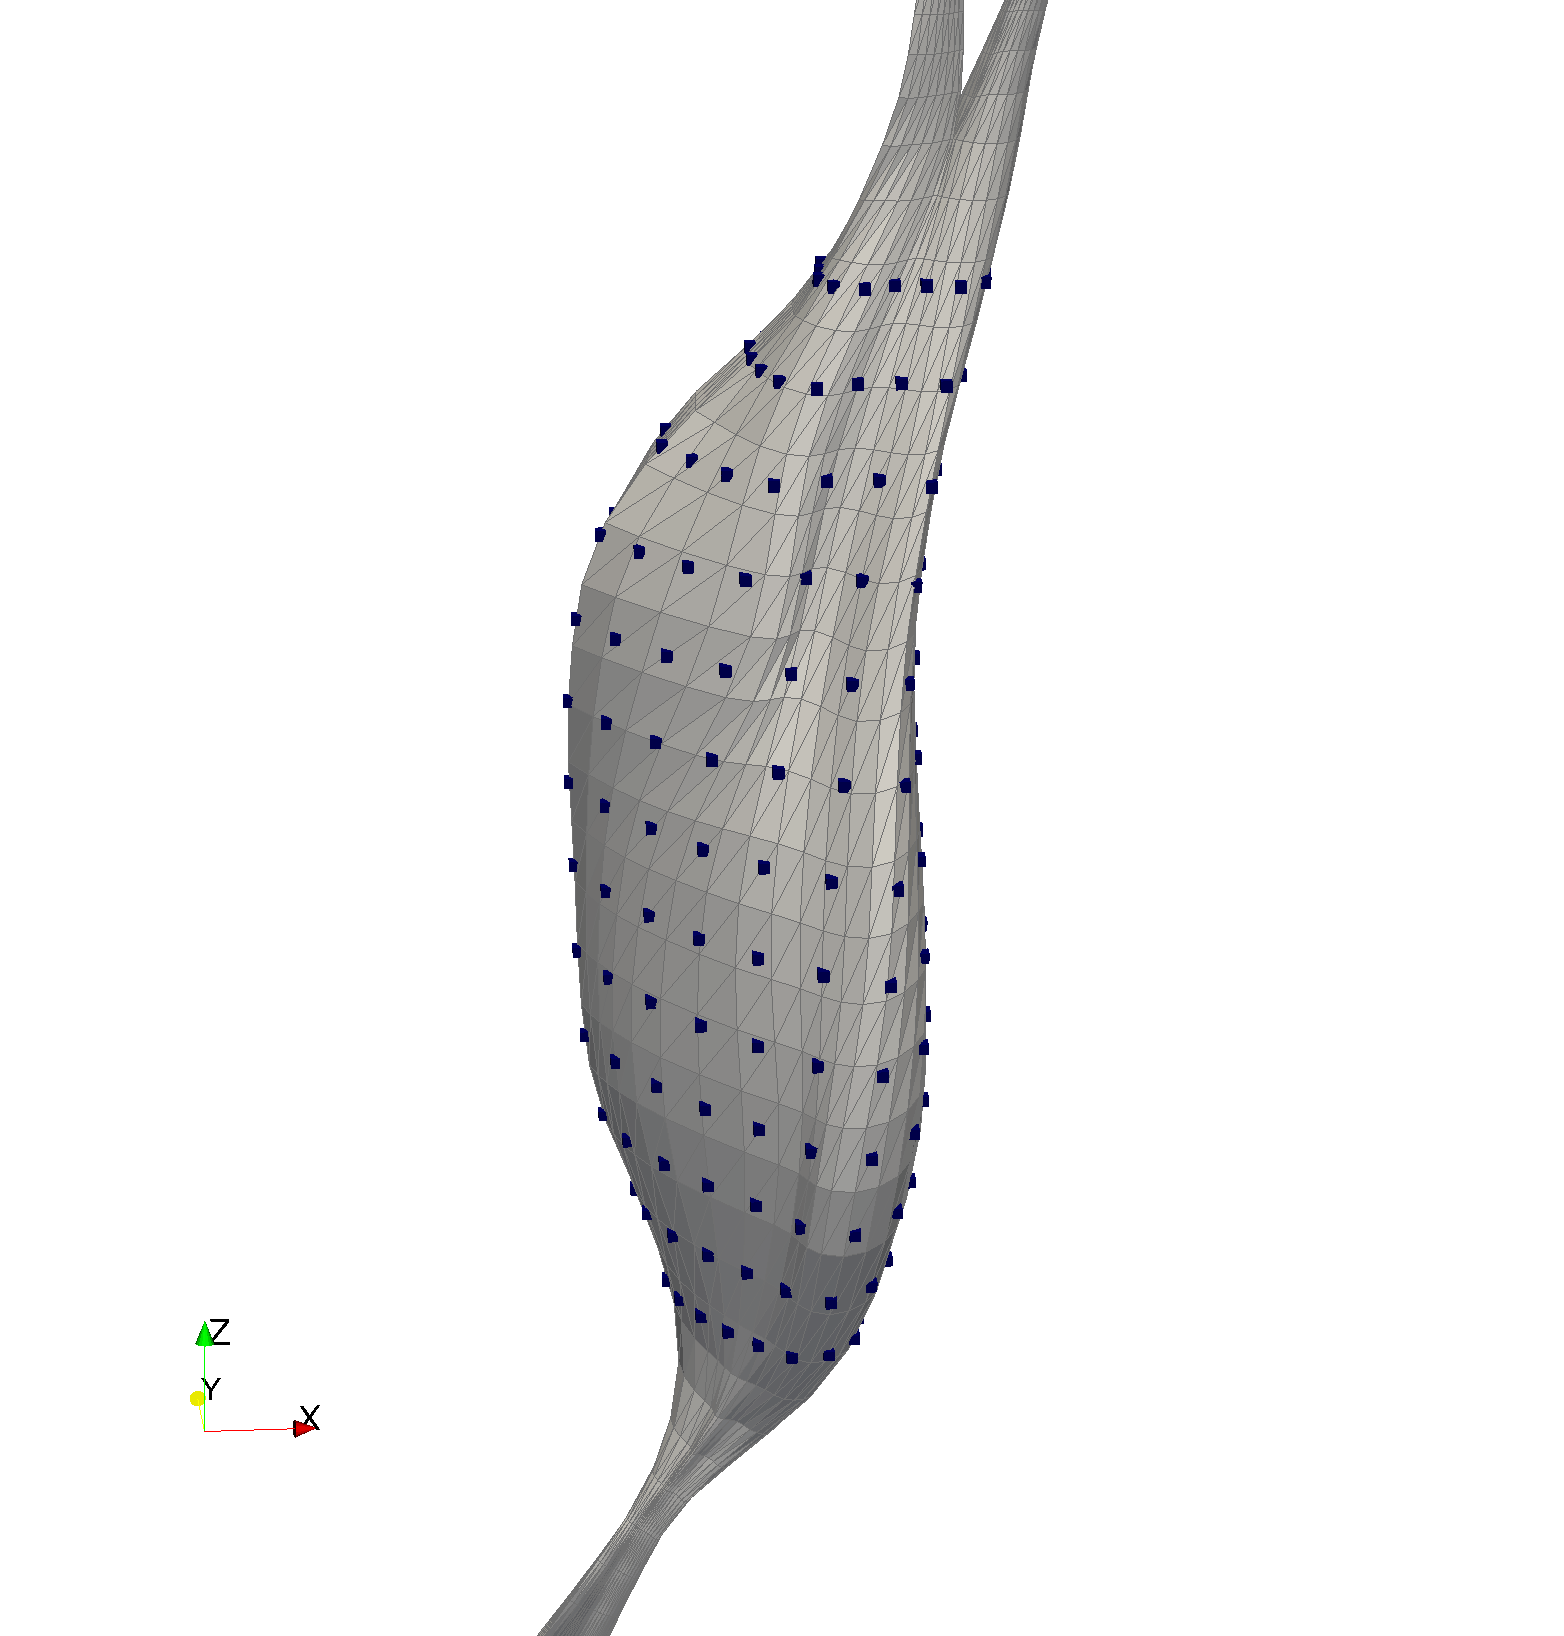
\includegraphics[height=10cm]{images/fiber_creation/serial_alg_0.png}% [trim=left bottom right top, clip]
    \caption{Extracted border points (blue) on the biceps surface mesh (gray). This is the result of line \algref{alg:serial_algorithm_1}{alg:1.1}.}%
    \label{fig:serial_alg_0}%
  \end{subfigure}
  \quad
  \begin{subfigure}[t]{0.48\textwidth}%
    \centering%
    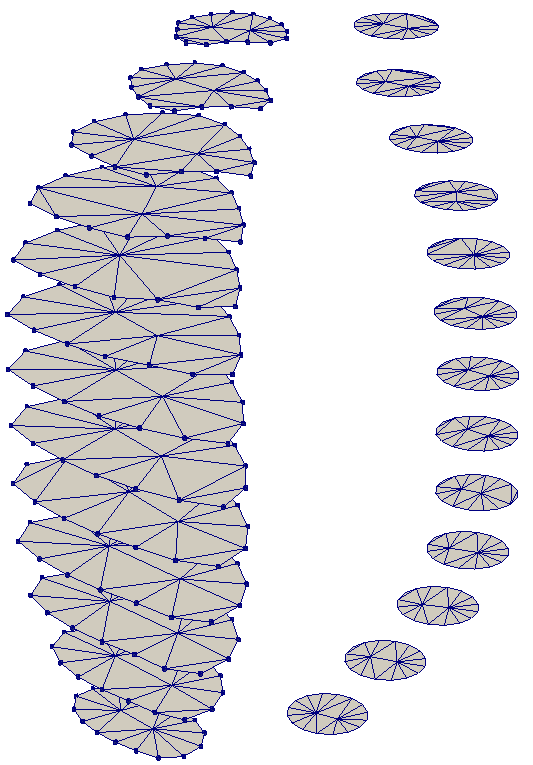
\includegraphics[height=10cm]{images/fiber_creation/serial_alg_3.png}%
    \caption{The generated triangulation of the slices (left) and the image $\bfy(\bfx)$ of the triangulation under the harmonic map (right). This figure shows the result of lines \algref{alg:serial_algorithm_1}{alg:1.2} and \algref{alg:serial_algorithm_1}{alg:1.3}.}%
    \label{fig:serial_alg_3}%
  \end{subfigure}\\
  \centering%
  \begin{subfigure}[t]{0.49\textwidth}%
    \centering%
    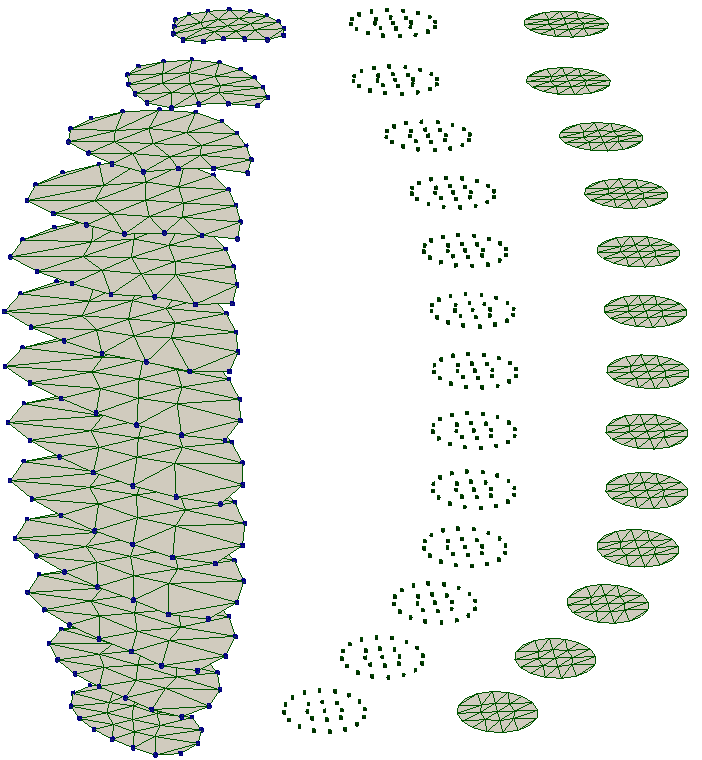
\includegraphics[height=10cm]{images/fiber_creation/serial_alg_4.png}%
    \caption{Grid in parameter space (right) and muscle domain (left), result after line \algref{alg:serial_algorithm_1}{alg:1.4}.}%
    \label{fig:serial_alg_4}%
  \end{subfigure}
  \hfill{}
  \begin{subfigure}[t]{0.4\textwidth}%
    \centering%
    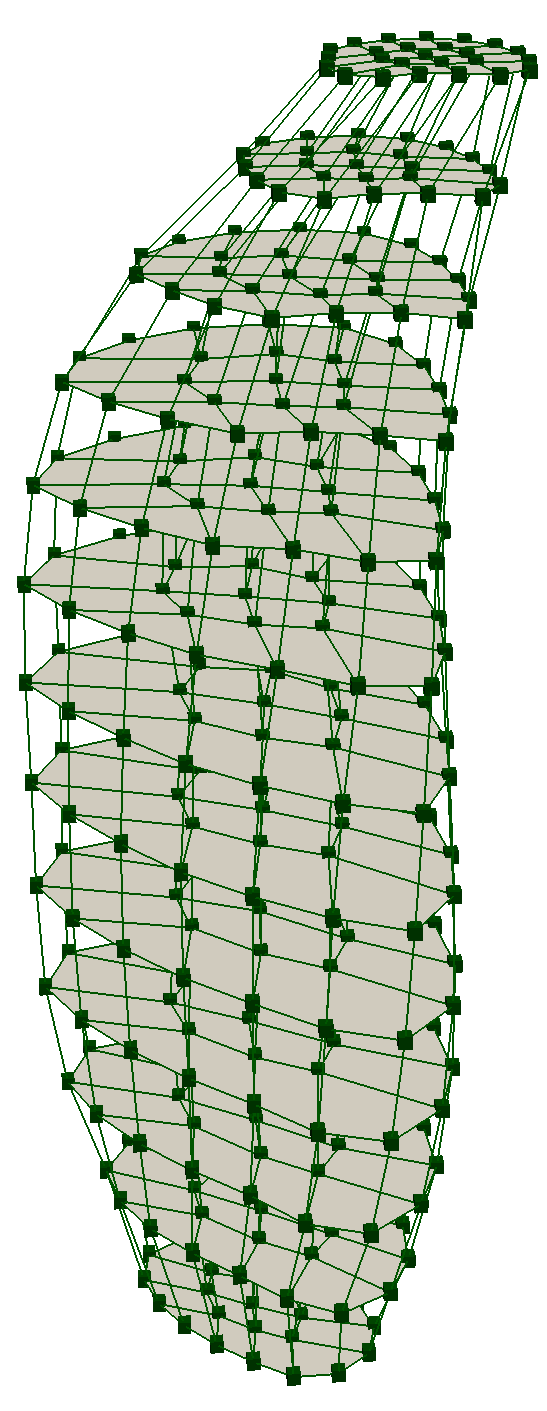
\includegraphics[height=10cm]{images/fiber_creation/serial_alg_8.png}%
    \caption{3D elements formed by connecting the slices, result after line \algref{alg:serial_algorithm_1}{alg:1.5}.}%
    \label{fig:serial_alg_8}%
  \end{subfigure}
  \caption{Steps of the serial algorithm, \cref{alg:serial_algorithm_1}, executed directly on the surface mesh of the biceps muscle (not the B-spline surface).}%
  \label{fig:serial_alg}%
\end{figure}%
%

\subsection{Triangulation of the Slices}
The points of each ring enclose a planar, polygonal surface, a \say{slice} $S_M$ of the muscle.
The next step in the algorithm, line \algref{alg:serial_algorithm_1}{alg:1.2}, is to triangulate the extracted slices, i.e. construct triangles that decompose the polygons. This is visualized at the left side in \cref{fig:serial_alg_3}.

Three different methods have been selected to construct the triangulation. The first and second methods are based on Delaunay triangulations, the third method constructs a custom triangulation.
\Cref{fig:triangulations} visualizes results of the three methods.

The first method uses the Delaunay tesselation algorithm from the spatial algorithms and data structures module of the Python package SciPy. The Quickhull algorithm \cite{quickhull} is used which triangulates the convex hull of the points. In consequence, the triangulation of concave slices have triangles that lie outside the interior of the slice. An advantage is that the triangulation uses all given points and no new points are added.

The example in \cref{fig:triangulation_0} shows a concave slice. At the bottom of the domain, the triangles are outside the slice and almost degenerate.

The second method uses a Delaunay refinement algorithm described in \cite{Delaunay2002} and implementated in the \emph{Triangle} software \cite{shewchuk96b}. A conforming, constrained Delaunay triangulation is created. The triangulation correctly handles convex and concave domains.
Conforming means that the triangulation uses the given points at the border. Additional points at the border as well as in the interior are added. The triangulation is constraint to generate triangles with minimum angles of 20 degrees and a maximum area $A$ that is set to a value dependend on the area of the bounding box. In consequence, all generated triangulations have a guaranteed mesh quality in terms of angles and about the same size and number of triangles.

Comparing the result of the second method in \cref{fig:triangulation_1} with the result of the first method in \cref{fig:triangulation_0} shows the better triangulation quality as the triangles all have higher angles.

The third method places one additional point in the center of gravity of the given points. Triangles are constructed by connecting the center point with two adjacent points on the border, for all given points. The resulting triangulation resembles a pie chart. For some concave slices, this method also creates triangles that partly lie outside the slice. The advantage of this approach is its simplicity.

\Cref{fig:triangulation_2} shows the result for an exemplary slice. Here, in contrast to the first method, the third method creates a valid triangulation despite the concave domain.

\begin{figure}%
  \centering%
  \begin{subfigure}[t]{0.31\textwidth}%
    \centering%
    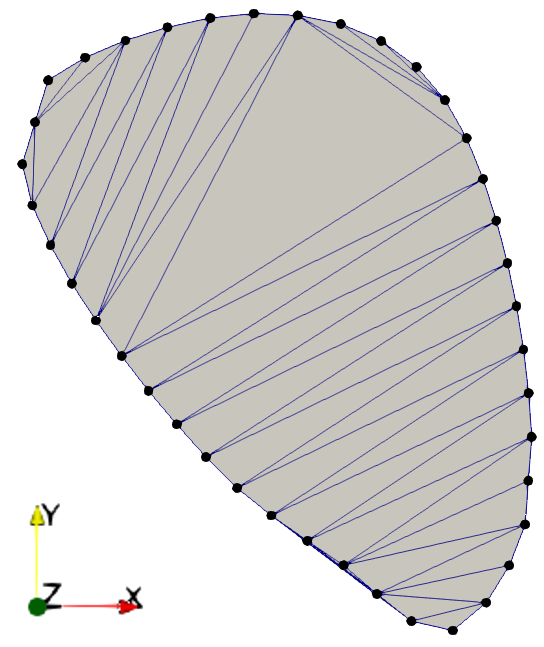
\includegraphics[width=\textwidth]{images/fiber_creation/triangulation_0.png}%
    \caption{First triangulation method}%
    \label{fig:triangulation_0}%
  \end{subfigure}
  \quad
  \begin{subfigure}[t]{0.31\textwidth}%
    \centering%
    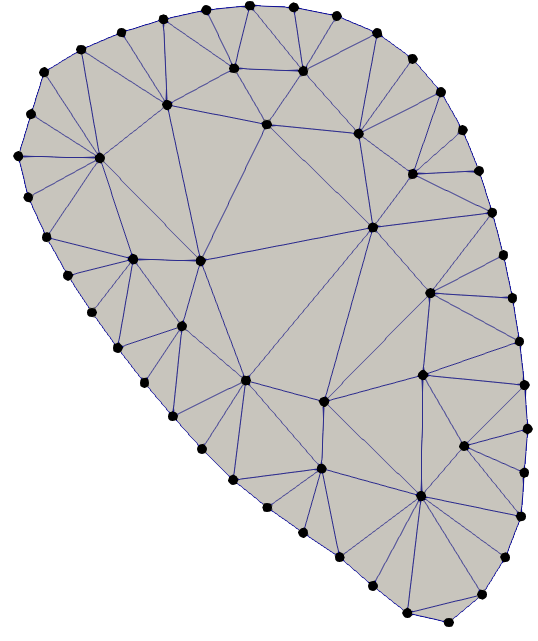
\includegraphics[width=\textwidth]{images/fiber_creation/triangulation_1.png}%
    \caption{Second trian\-gulation method}%
    \label{fig:triangulation_1}%
  \end{subfigure}
  \quad
  \begin{subfigure}[t]{0.31\textwidth}%
    \centering%
    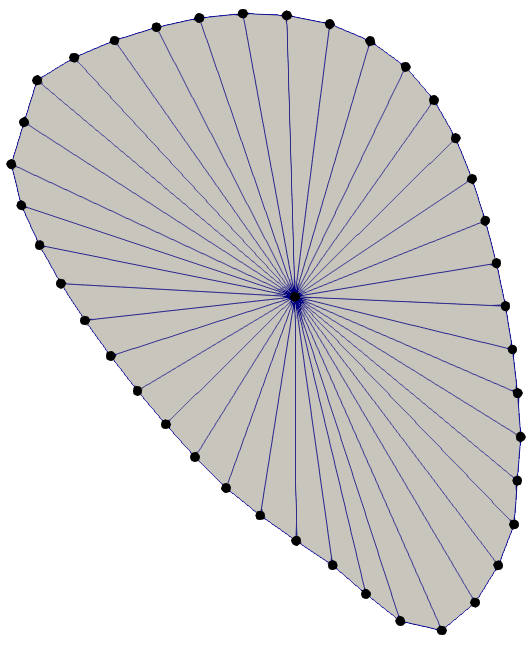
\includegraphics[width=\textwidth]{images/fiber_creation/triangulation_2.png}%
    \caption{Third triangulation method}%
    \label{fig:triangulation_2}%
  \end{subfigure}
  \caption{Result of different triangulation methods for a slice in the center of the biceps muscle.}%
  \label{fig:triangulations}%
\end{figure}%

\subsection{Harmonic Maps}
The next step is line \algref{alg:serial_algorithm_1}{alg:1.3}, compute the harmonic maps $u$ and $v$. For a given slice $S_M$, these functions map from $S_M$ to coordinates $u,v\in \R$ of a parameter domain $\Omega_P \subset \R^2$. The parameter domain is either a unit circle or a unit square.

The vector $\bfy(\bfx) := (u(\bfx), v(\bfx))^\top$ for $\bfx \in S_M$ is interpreted as position in $\Omega_P$. The maps are constructed such that the border $∂S_M$ of the slice $S_M$ is evenly mapped to the border $∂\Omega_P$ of the parameter domain $\Omega_P$.
The mapping $\bfy: S_M \to \Omega_P$ is bijective and harmonic, i.e. the Laplace operator of $u$ and $v$ is zero.

More specifically, the definition is
%
\begin{equation}\label{eq:def_harmonic_maps}
  \begin{array}{l}
    u : S_M \to \R, \quad v : S_M \to \R,\\[4mm]
    Δu(\bfy) = 0, \quad Δv(\bfy) = 0 \quad \forall \bfy \in S_M.
  \end{array}
\end{equation}
%
For a uniform parametrization $\bfp:[0,1] \to ∂S_M$ of the border $∂S_M$ of the slice, i.e., 
%
\begin{align*}
  \p{l(t)}{t} = c \in \R \quad \forall t \in [0,1], \quad \text{where } l(t) := \i{0}{t} |\bfp'(\tau)| \,\d\tau,
\end{align*}
%
we require the mapping of the parametrization to be also uniform, i.e.,%
\begin{align*}
  \p{l_P(t)}{t} = c_P \in \R \quad \forall t \in [0,1], \quad \text{where } l_P(t) := \i{0}{t} |\bfy'\big(\bfp(\tau\big)| \,\d\tau.
\end{align*}
%
This leads to the following Dirichlet boundary conditions that close the definition in \cref{eq:def_harmonic_maps}:%
\begin{align}\label{eq:bc_harmonic_maps}
  u(\bfx_\text{M,border}) = u_\text{P,border}, \quad v(\bfx_\text{M,border}) = v_\text{P,border}.
\end{align}
%

\Cref{eq:def_harmonic_maps,eq:def_harmonic_maps} describes a boundary value problem of ordinary differential equations in $u$ and $v$. We solve it using the Finite Element Method and the spatial discretization given by the triangulation of the slices.

The first step is to compute the prescribed border points in parameter space,\\
 ${(u_\text{P,border}, v_\text{P,border})^\top}$. When using the first and third triangulation methods, the border points on the slices are  equidistant and therefore the same number of points need to be sampled equidistantly on the border $∂\Omega_P$ of the parameter space.
If the second triangulation method which added additional points is used, also the same number of points  are created on the border $∂\Omega_P$ of the slice as are given on the slice $∂S_M$. The border points are created such that the relations of their distances is the same on $∂\Omega_P$ as for the original points on $∂S_M$.

Using the standard procedure of the Finite Element method for $\nabla u(\bfx) = 0$ on $S_M$ and $u=f(\bfx)$ on $∂S_M$, e.g. as outlined in \cite{Remacle2010}, leads to the weak form with ansatz and test functions $\phi$,
\begin{align}\label{eq:est_fe_w}
    \i{S_M}{} (\nabla u^\top \nabla \phi + \nabla f(\bfx)^\top \nabla \phi) \,\d \bfx = 0 \quad \forall \phi \in \mathcal{H}_0^1.
\end{align}
Standard linear hat functions are used on the triangles with the interpolation property $\phi_i(\bfx_j) = \delta_{ij}$. Using the barycentric parametrization of triangles with points $\bfp^1,\bfp^2$ and $\bfp^3$ introduced in \cref{eq:barycentric_triangle} we get for the ansatz functions and their derivatives within the elements
%
\begin{align*}
  \phi^{(e)}_1 &= (1 - \xi_1)(1 - \xi_2), \quad&
  \phi^{(e)}_2 &= \xi_1 (1 - \xi_2), \quad &
  \phi^{(e)}_3 &= (1 - \xi_1) \xi_2,\\[4mm]
  \nabla \phi^{(e)}_1 &= (\xi_2-1, \xi_1 - 1)^\top, \quad&
  \nabla \phi^{(e)}_2 &= (1-\xi_2, -\xi_1)^\top, \quad&
  \nabla \phi^{(e)}_3 &= (-\xi_2, 1-\xi_1)^\top.
\end{align*}
The superscript $\square^{(e)}$ refers to the definition of the functions within elements. The usual global assembly involves composing the global, nodal functions $\phi_i(\bfx)$ for nodes indexed by $i=1, \dots, n_\text{nodes}$ and using a mapping between the barycentric coordinates $\xi_1,\xi_2 \in [0,1]^2$ inside the elements to the global coordinates $\bfx \in S_M$.

Inserting the discretization
\begin{align*}
  u_h(\bfx) = \s{i=1}{n_\text{nodes}} u_i\,\phi_i(\xi_1(\bfx), \xi_2(\bfx))
\end{align*}
into \cref{eq:est_fe_w} leads to the form
\begin{equation}\label{eq:est_weak_form}
  \begin{array}{lll}
    \s{i=1}{n_\text{nodes}}u_i \i{S_M}{} \nabla_\bfx \phi_i^\top \nabla_\bfx \phi_j \,\d\bfx + \s{i=1}{n_\text{nodes}} f_i \i{S_M}{} \nabla_\bfx \phi_i^\top \nabla_\bfx \phi_j \,\d \bfx = 0\,\quad \forall j=1,\dots,n_\text{nodes}.
  \end{array}
\end{equation}
The integrations are executed element-wise and over the elemental coordinates $\xi_1,\xi_2$. 

The transformation to elemental coordinates involves the computation of the Jacobian $J=\d\bfx/\d\bfxi$ of the mapping between element coordinates $\bfxi = (ξ_1,ξ_2)$ and global coordinates $\bfx$. From the definition \cref{eq:barycentric_triangle} it follows that
\begin{align*}
  J = \d{\bfx}{\bfxi} = [\bfp^2-\bfp^1, \bfp^3-\bfp^1].\\[4mm]
\end{align*}
The metric tensor for this mapping is given by
\begin{align*}
  \mathcal{M} := \left(\d{x}{\bfxi}\right)^T \, \left(\d{x}{\bfxi}\right).
\end{align*}
%
The transformation of the integrals in \cref{eq:est_weak_form} introduces an additional integration factor of $\sqrt{\det{\mathcal{M}}}$.

We get the following matrix equation:
\begin{align}\label{eq:est_fe_system}
  M_u \bfu = -M_f\,\bff,
\end{align}
with the vector $\bfu$ of nodal solution values, the vector $\bff$ of nodal Dirichlet boundary condition values at the border and the global stiffness matrices $M_u$ and $M_f$. The two global stiffness matrices are assembled from the element stiffness matrices $M^\text{el}$ for the degrees of freedom at all nodes respectively at the border nodes. The entries of the element stiffness matrices are given by
\begin{align*}
  M^\text{el}_{i,j} = \i{0}{1}\i{0}{1-\xi_1}   \nabla \phi_i^{(e)}(\xi_1,\xi_2)^\top \, \mathcal{M}^{-1} \, \nabla \phi_j^{(e)}(\xi_1,\xi_2) \, \sqrt{\det{\mathcal{M}}}  \,\d\xi_2\d\xi_1.
\end{align*}
By solving \cref{eq:est_fe_system} for $\bfu$ we get the discretized harmonic map $u$.
The Finite Element formulation and computation for $v$ is analogous and uses the same global stiffness matrices.

\Cref{fig:harmonic_map_solution} visualizes the triangulation of $S_M$ and the solutions $u(\bfx)$ and $v(\bfx)$ in the first two plots. The color range from bright yellow to dark violet corresponds increasing values of $u$ and $v$. It can be seen that the $u$ values increase from left to right whereas the $v$ values increase from bottom to top, corresponding to the horizontal and vertical coordinate axis $y_1$ and $y_2$ of $\Omega_P$.


Applying the computed harmonic map $\bfy(\bfx)$ to the triangulation of the slices results in a triangulation of the parameter domain $\Omega_P$. This is shown in the third plot of \cref{fig:harmonic_map_solution} and in \cref{fig:serial_alg_3}.
The generated triangulation of the slices was generated using the second triangulation method with the constrained Delaunay triangulation. On the right, the image $\bfy(\bfx)$ under the harmonic map of the triangulation in the slices is shown on the unit circle parameter domains.

\begin{figure}%
  \centering%
  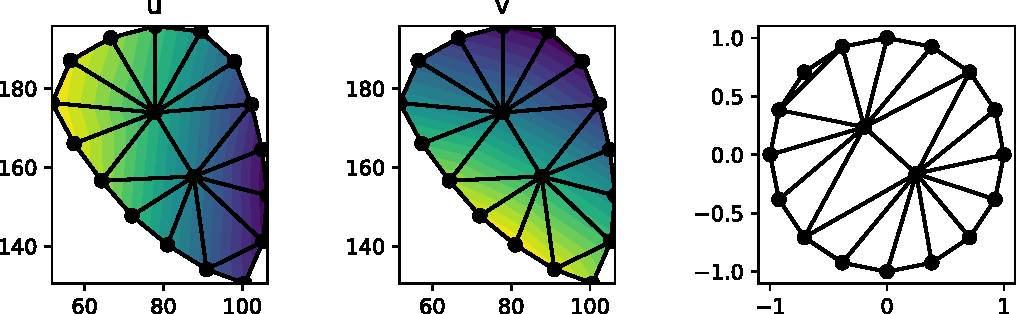
\includegraphics[width=\textwidth]{images/fiber_creation/harmonic_map_9b.pdf}%
  \caption{Triangulations and harmonic map for a slice $S_M$ of the biceps muscle. The first two plots show the solutions of $u$ and $v$ on the slice $S_M$. The third plot shows the image in $\Omega_P$ of the triangulation in $S_M$ under the harmonic map.}%
  \label{fig:harmonic_map_solution}%
\end{figure}%

\subsection{Construction of a regular grid in the parameter domain}
The next step in the \cref{alg:serial_algorithm_1} is the construction of a structured, regular grid in the parameter domain $\Omega_P$, as stated in line \algref{alg:serial_algorithm_1}{alg:1.4}. This grid will then be mapped to the slices $S_M$. Creating a structured grid in a given domain is also called \emph{quadrangulation}.

The parameter domain $\Omega_P$ can be selected to be either a unit square or a unit circle. For both choices, two different schemes how to generate a grid with given number of cells can be selected.
\Cref{fig:quads} shows all four possiblities.

The first scheme, \cref{fig:quad_1}, uses an equidistant regular grid. The grid will be mapped to a cross section of the muscle which has no sharp corners like the unit square. Therefore, the cells of the grid will be distorted at the corners, usually shortening diagonals that point towards the corners and stretching the other diagonals. This assumption motivates the second scheme in \cref{fig:quad_2}. Here, the elements are already distorted in the described manner, with increasing distortion closer to the corners.

A different approach is to use a unit circle, which has no corners and therefore might more resemble a muscle cross section. The first scheme of the unit circle is given in \cref{fig:quad_0}. It uses the radial and circumferential directions for the two dimensions of the grid. A disadvantage of this scheme is that the quadrilaterals at the center are degenerated to triangles. Additionally, the area of the cells varies significantly and the outer cells have unequal side lengths. To remedy this problem, the second scheme given in \cref{fig:quad_3} is constructed. When traversing from the outer border towards the center point and considering the circumferential lines of grid points, the circle morphs into a square as the number of grid points decreases. This approach has the disadvantage that some cells have an inner angle of nearly \SI{180}{\degree}, especially four elements at the border.

Each construction schemes allows to specify the (squared) number of nodes and in consequence the number of cells. The examples in \cref{fig:quad_1,fig:quad_2,fig:quad_3} have $11 \times 11$ nodes and $10 \times 10$ cells. For \cref{fig:quad_0}, the numbers are slightly different. There are $10 \times 11 + 1$ nodes resulting in $10 \times 11$ cells.

\begin{figure}%
  \centering%
  \begin{subfigure}[t]{0.48\textwidth}%
    \centering%
    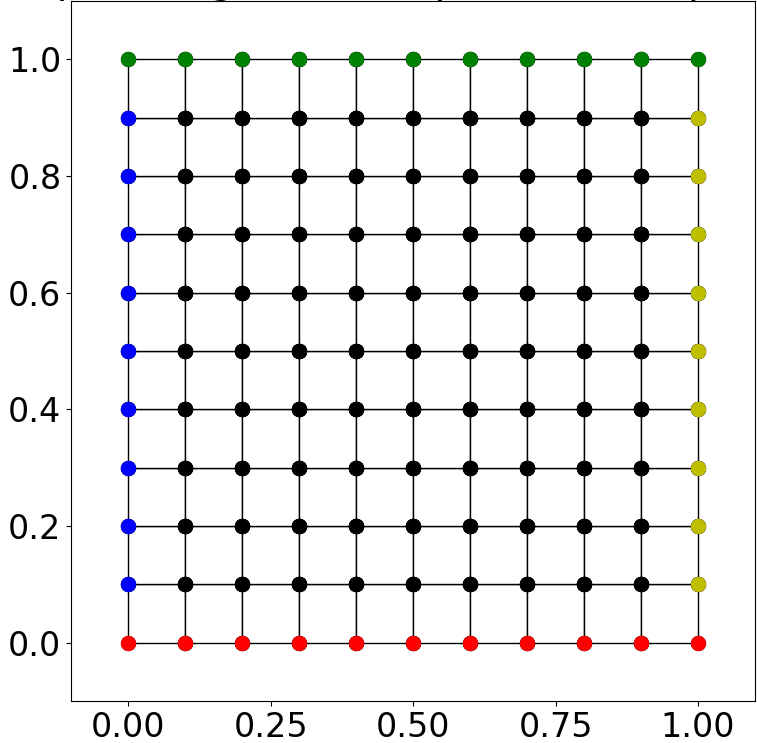
\includegraphics[width=\textwidth]{images/fiber_creation/quad_1.png}%
    \caption{Unit square, scheme 1}%
    \label{fig:quad_1}%
  \end{subfigure}
  \quad
  \begin{subfigure}[t]{0.48\textwidth}%
    \centering%
    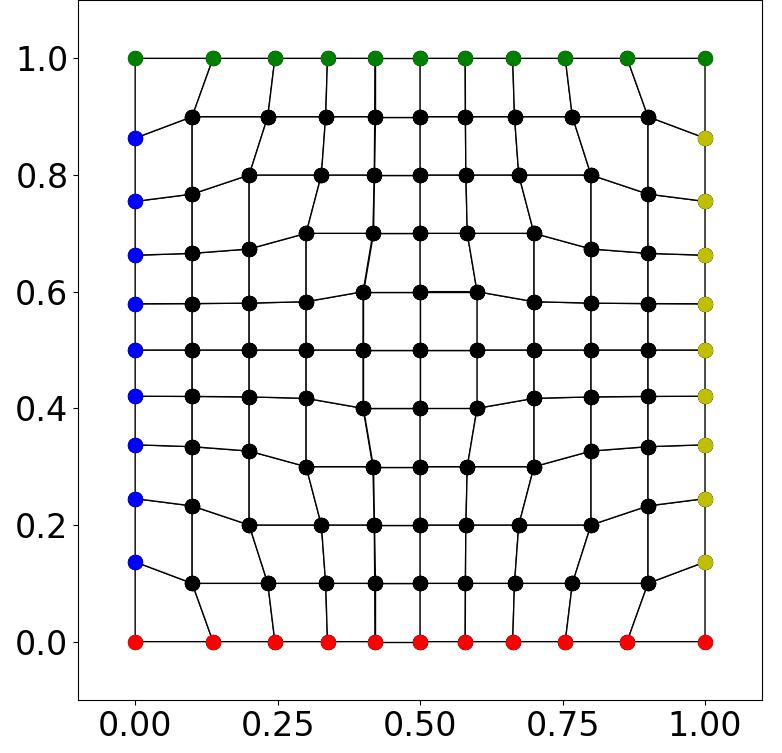
\includegraphics[width=\textwidth]{images/fiber_creation/quad_2.png}%
    \caption{Unit square, scheme 2}%
    \label{fig:quad_2}%
  \end{subfigure}
  \begin{subfigure}[t]{0.48\textwidth}%
    \centering%
    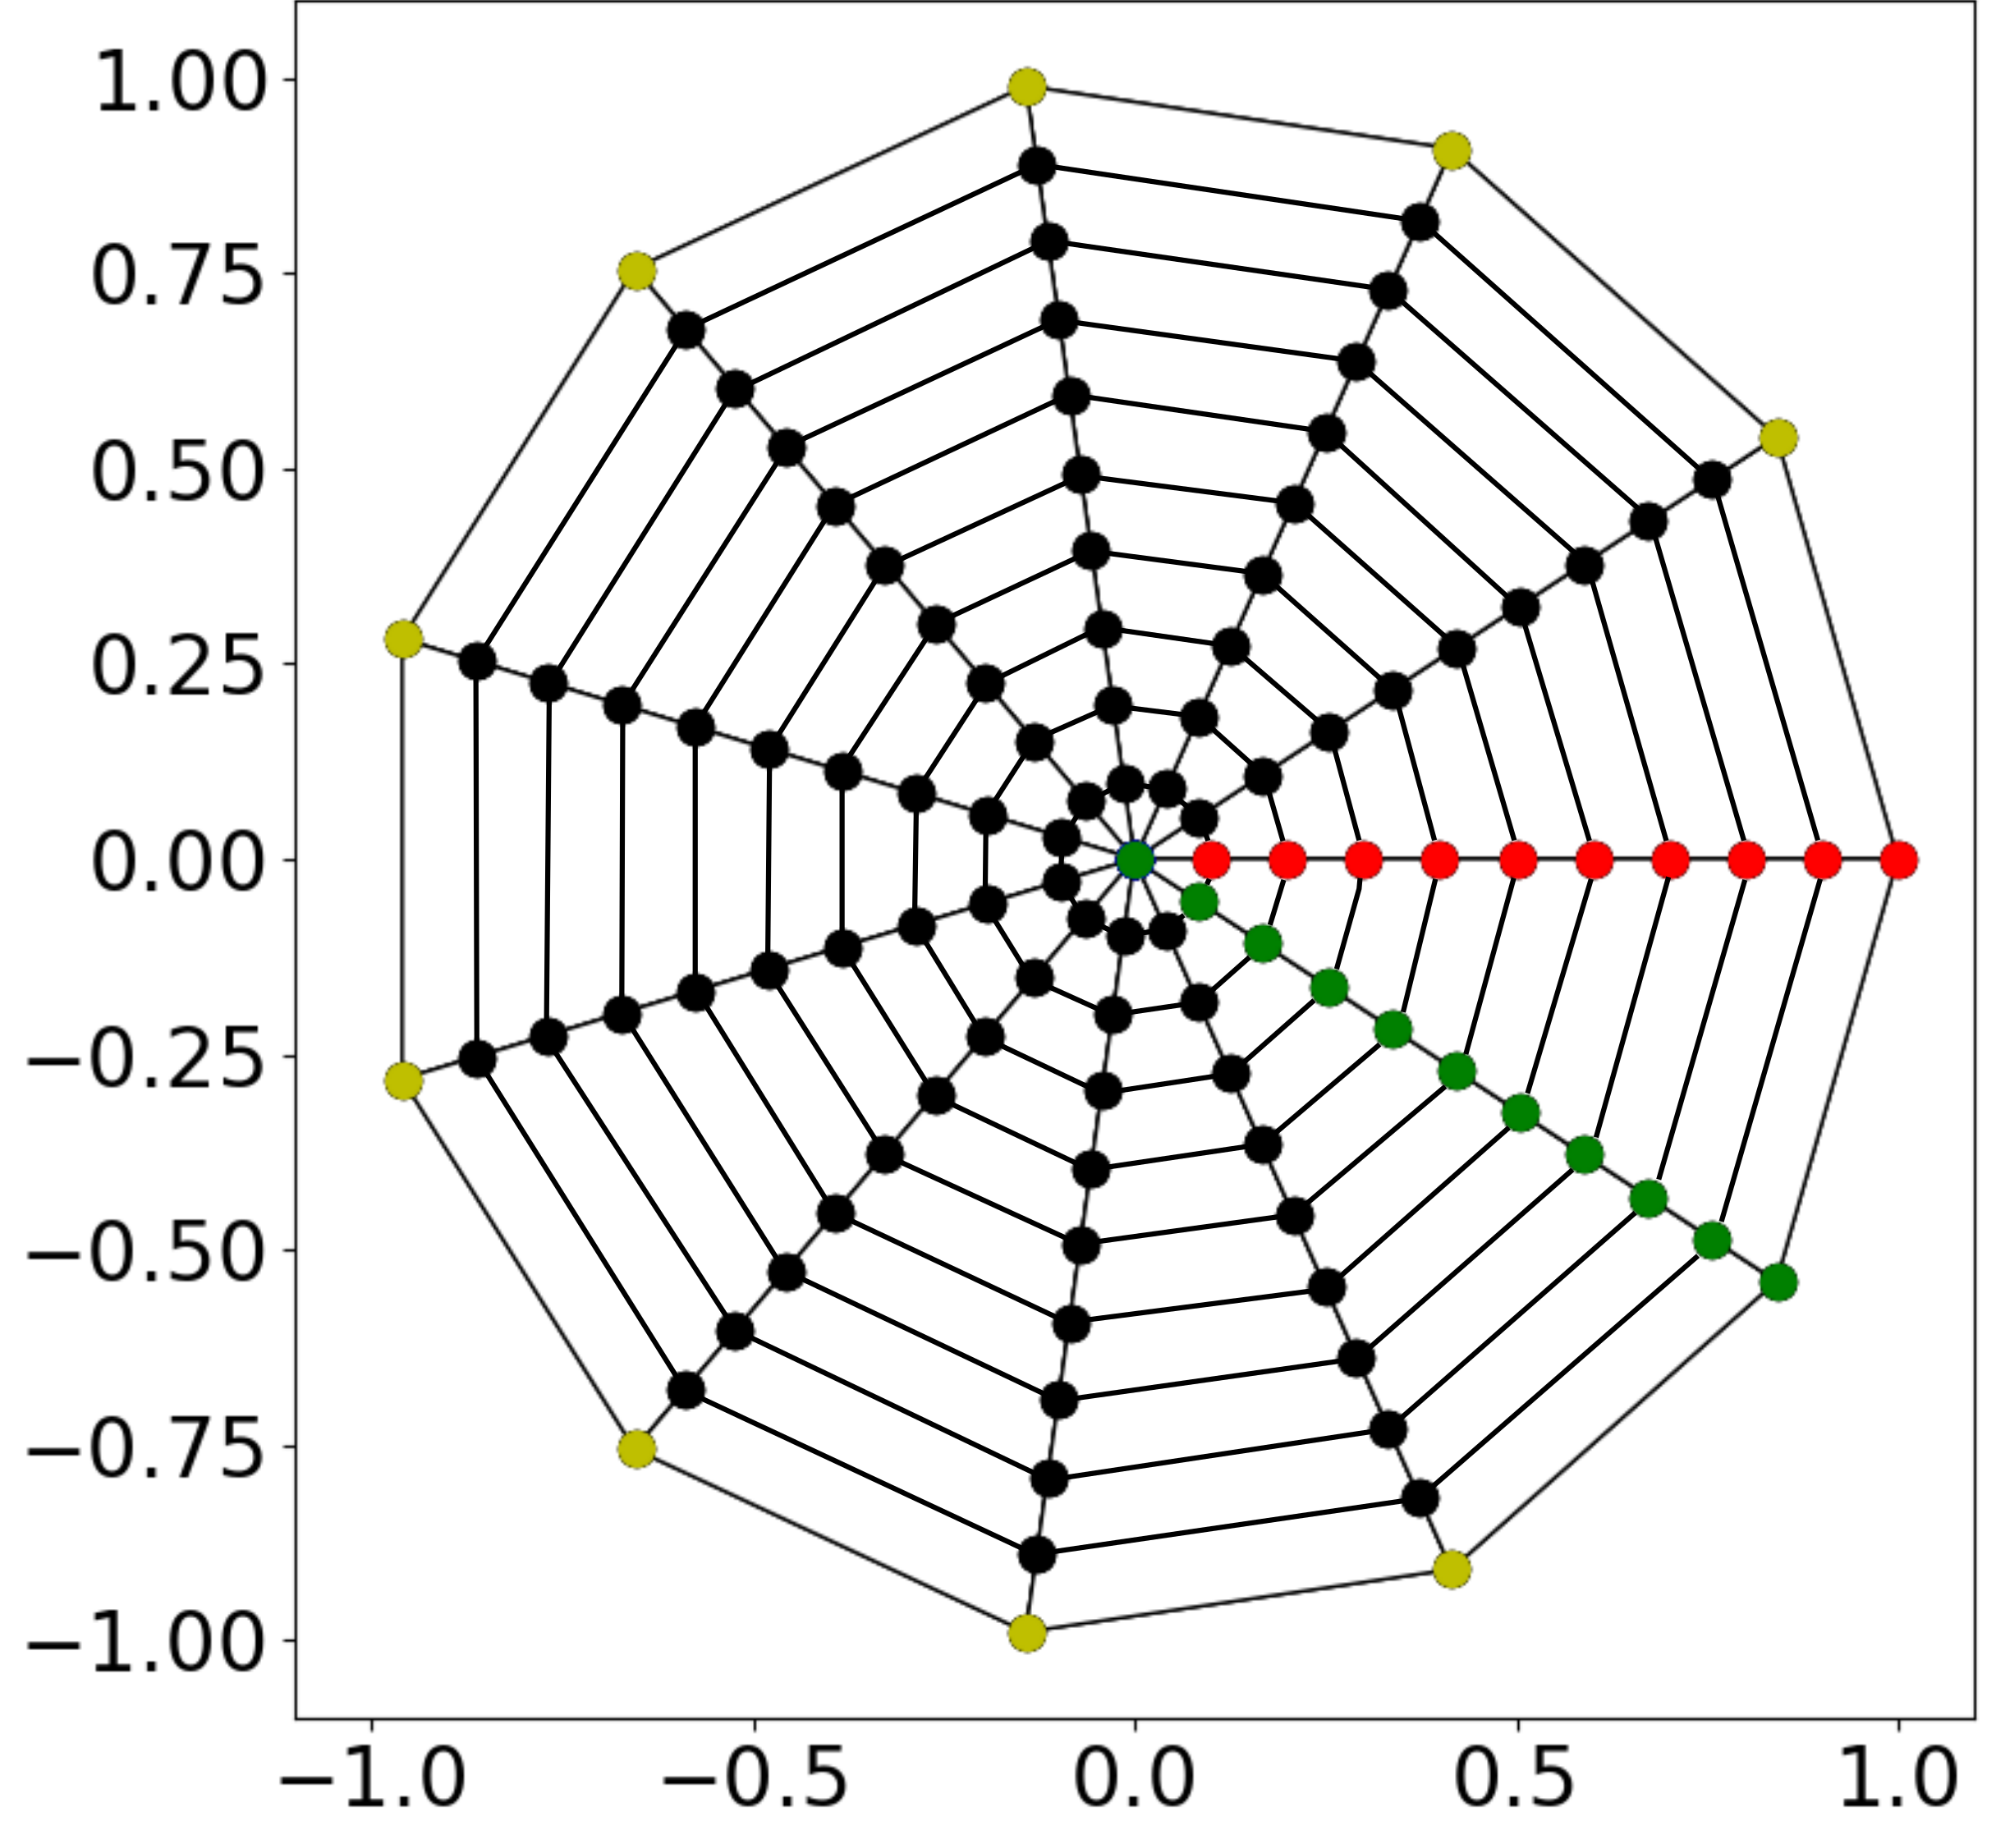
\includegraphics[width=\textwidth]{images/fiber_creation/quad_0.png}%
    \caption{Unit circle, scheme 1}%
    \label{fig:quad_0}%
  \end{subfigure}
  \quad
  \begin{subfigure}[t]{0.48\textwidth}%
    \centering%
    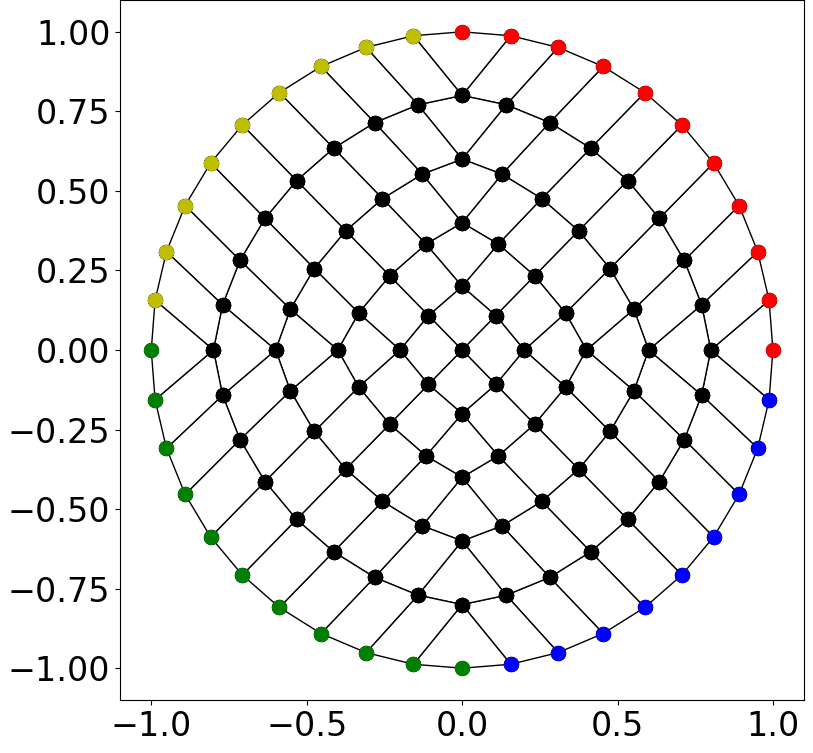
\includegraphics[width=\textwidth]{images/fiber_creation/quad_3.png}%
    \caption{Unit circle, scheme 2}%
    \label{fig:quad_3}%
  \end{subfigure}
  \caption{Different quadrangulation schemes of the parameter domain with $11\times 11$ nodes. The borders of the grid are colored for better perceptiblity.}%
  \label{fig:quads}%
\end{figure}%

Next, the grid in the parameter domain is transferred to the muscle domain by applying the harmonic map $\bfy(\bfx) \in S_M$ on every point of the quadrangulation $\bfx \in \Omega_P$. This is illustrated in \cref{fig:serial_alg_4} for a parameter domain consisting of the unit circle, with quadrangulation scheme 2 and $5 \times 5$ nodes. The cells of the grid in $\Omega_P$ are shown in the right-most stack of domains. The grid points are visualized left of the grids. The resulting image of the mesh in the slices $S_M$ is shown on the left. For visualization reasons, each quadrilateral has been split into two triangles.

\subsection{Formation of Three-Dimensional Elements}

The result of the previous steps is a number of quadrangulated muscle slices. The grid on every slice has the same number of nodes and elements. The nodes on the border of neighbouring slices are positioned similarly.

The final step of \cref{alg:serial_algorithm_1} is line \algref{alg:serial_algorithm_1}{alg:1.5}, the formation of 3D elements. Inserting edges between all corresponding nodes on two neighbouring slices creates a set of 3D elements and, thus, an overall 3D quadrilateral mesh of the muscle volume. This step is visualized in \cref{fig:serial_alg_8}.

\subsection{Generation of Fiber Meshes}

% idea, literature
% Laplace, BC, FEM
% Computation of gradient
% Streamlines in gradient
% resampling

\begin{algorithm}
  \begin{algorithmic}[1]%
    \Statex\Procedure{Create\_1D\_meshes}{}
    \Require structured 3D volume mesh
    \Ensure 1D fiber meshes
    \Statex
    \State Solve Laplacian flow problem
    \State Trace streamlines in the gradient field
    \State Sample 1D fiber meshes
    \EndProcedure
  \end{algorithmic}%
  \caption{Serial algorithm}%
  \label{alg:serial_algorithm_2}%
\end{algorithm}%



\begin{figure}%
  \centering%
  \begin{subfigure}[t]{0.49\textwidth}%
    \centering%
    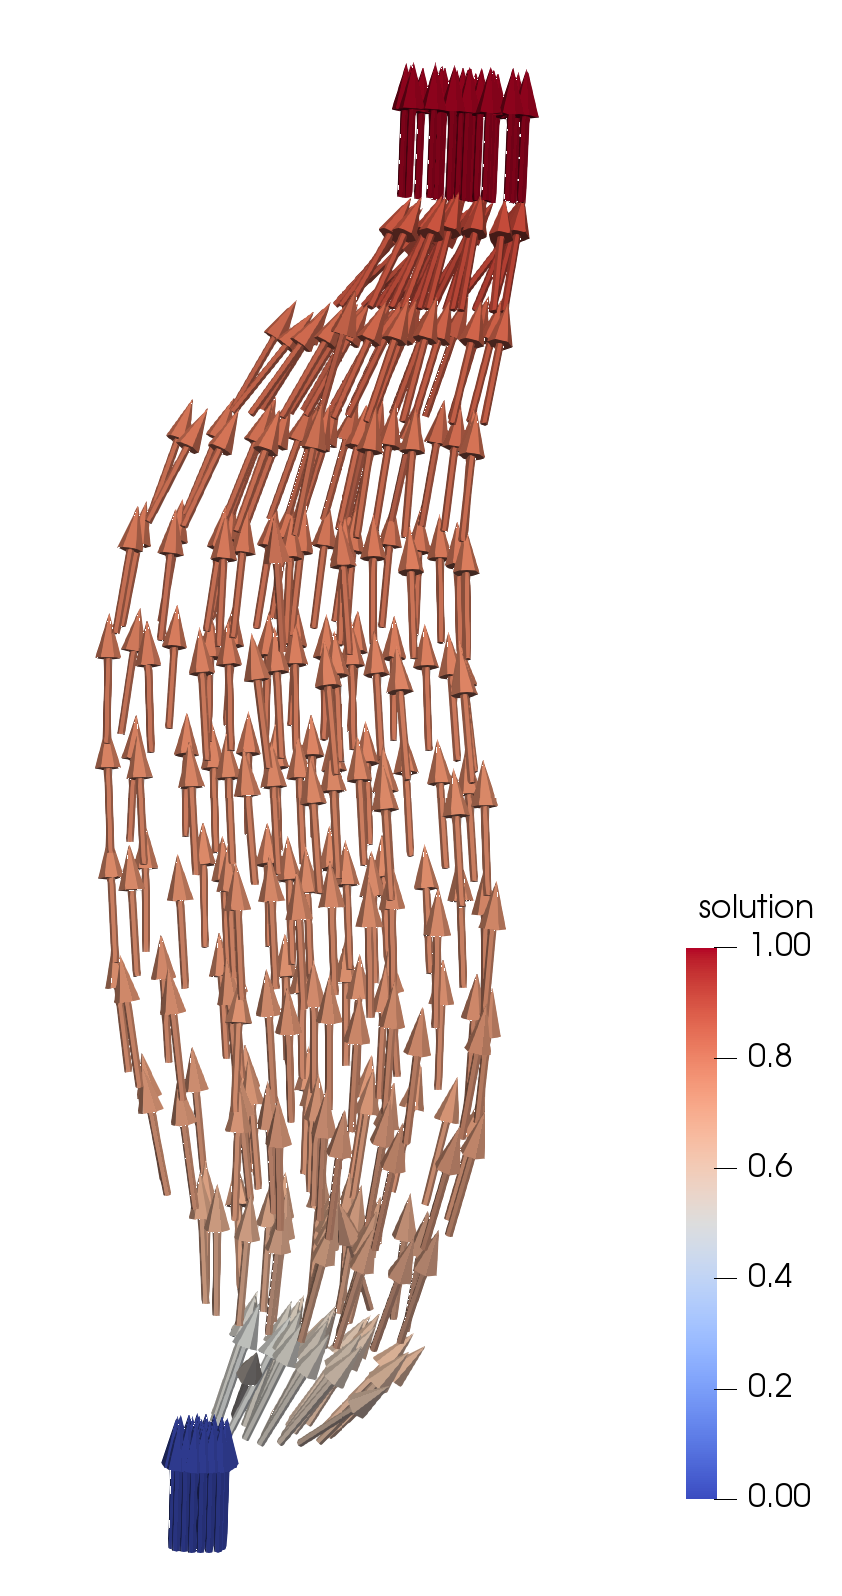
\includegraphics[height=10cm]{images/fiber_creation/potential_flow.png}%
    \caption{}%
    \label{fig:potential_flow}%
  \end{subfigure}
  \begin{subfigure}[t]{0.49\textwidth}%
    \centering%
    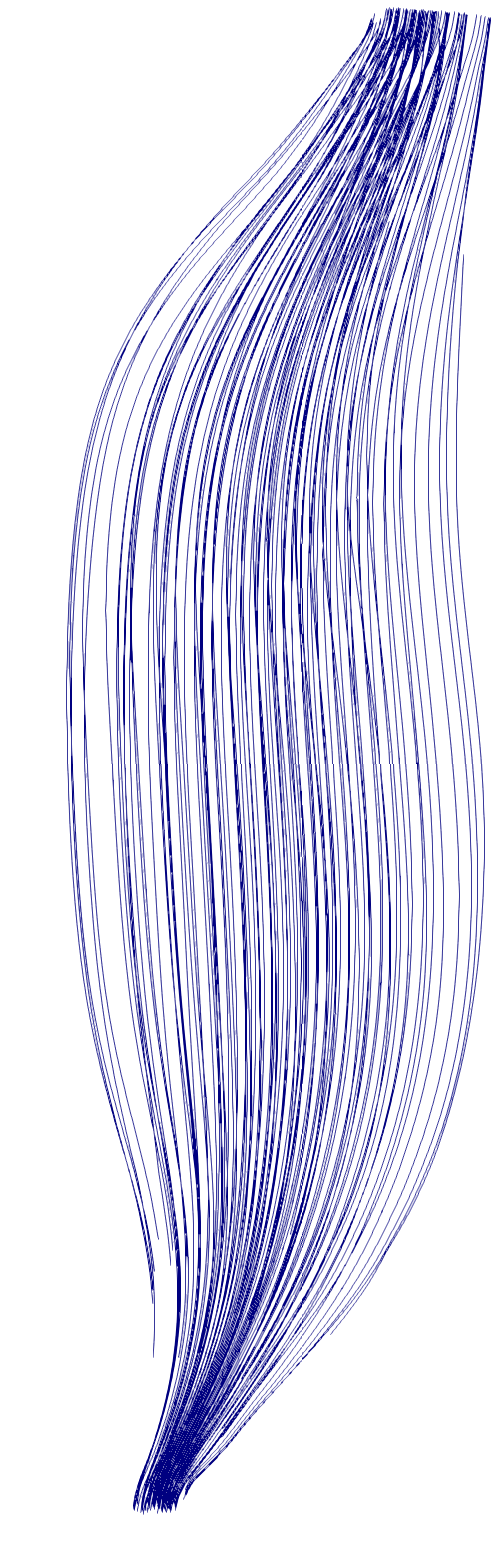
\includegraphics[height=10cm]{images/fiber_creation/streamlines.png}%
    \caption{}%
    \label{fig:streamlines}%
  \end{subfigure}
  \caption{.}%
  \label{fig:potential_flow_streamlines}%
\end{figure}%
%


\subsection{Results and Discussion}

% ------------------
% parameter space triangulations
\begin{figure}%
  \centering%
  \begin{subfigure}[t]{0.31\textwidth}%
    \centering%
    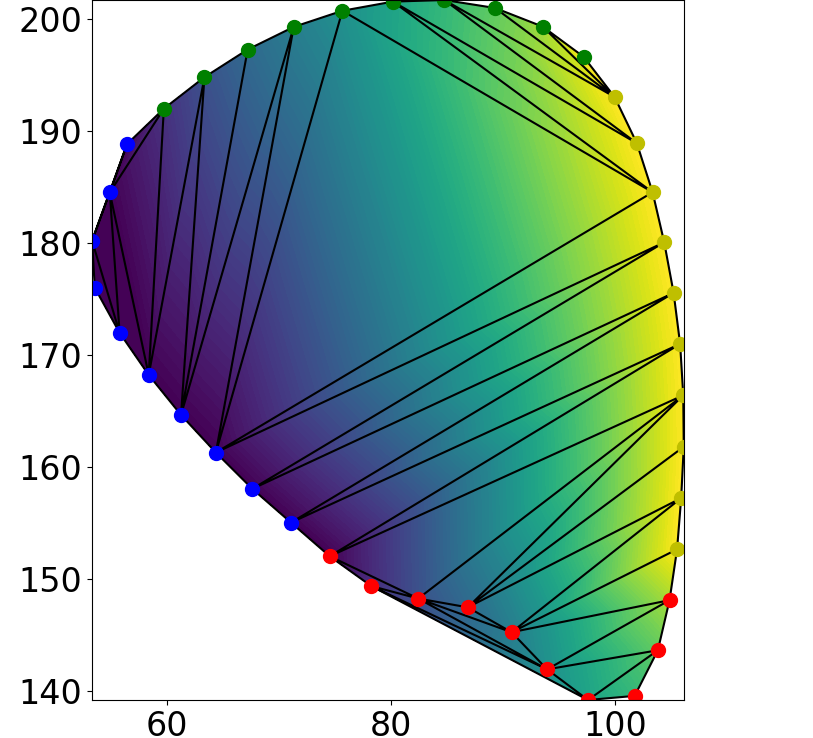
\includegraphics[width=\textwidth]{images/fiber_creation/u_0.png}%
    \caption{First method}%
    \label{fig:triu_0}%
  \end{subfigure}
  \quad
  \begin{subfigure}[t]{0.31\textwidth}%
    \centering%
    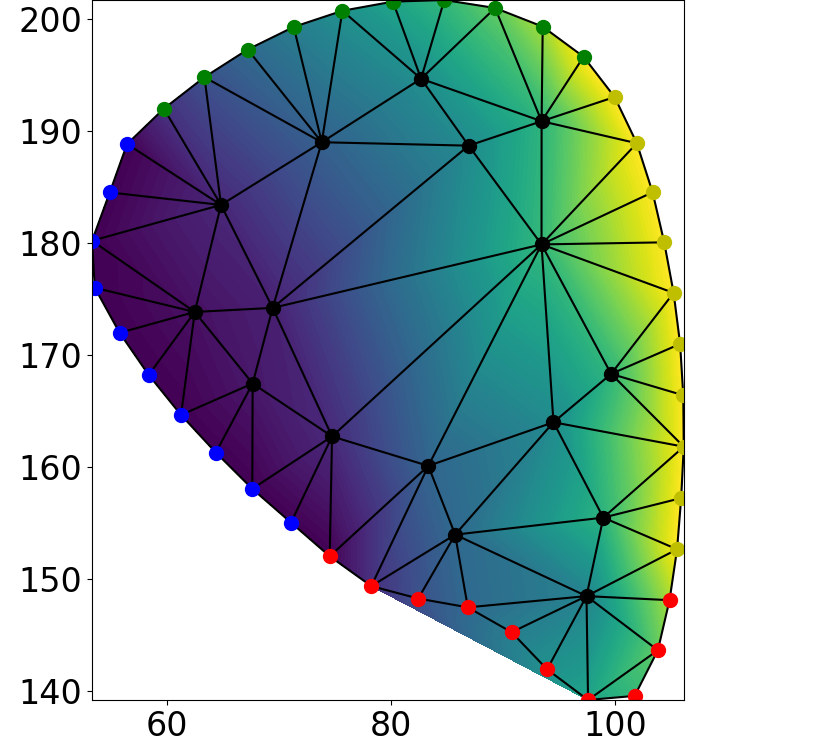
\includegraphics[width=\textwidth]{images/fiber_creation/u_1.png}%
    \caption{Second method}%
    \label{fig:triu_1}%
  \end{subfigure}
  \quad
  \begin{subfigure}[t]{0.31\textwidth}%
    \centering%
    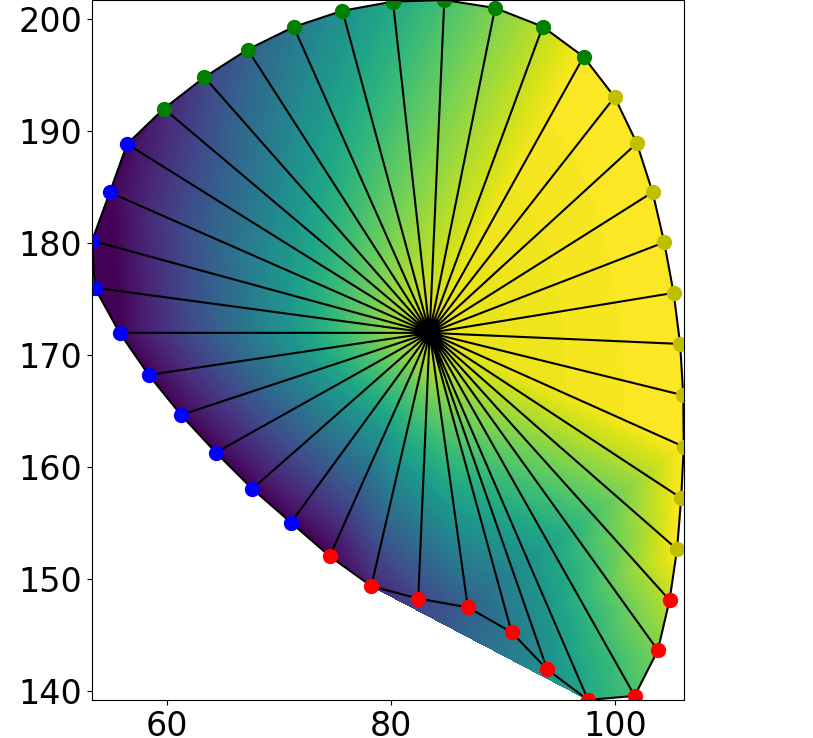
\includegraphics[width=\textwidth]{images/fiber_creation/u_2.png}%
    \caption{Third method}%
    \label{fig:triu_2}%
  \end{subfigure}\\
  
  % square
  \begin{subfigure}[t]{0.31\textwidth}%
    \centering%
    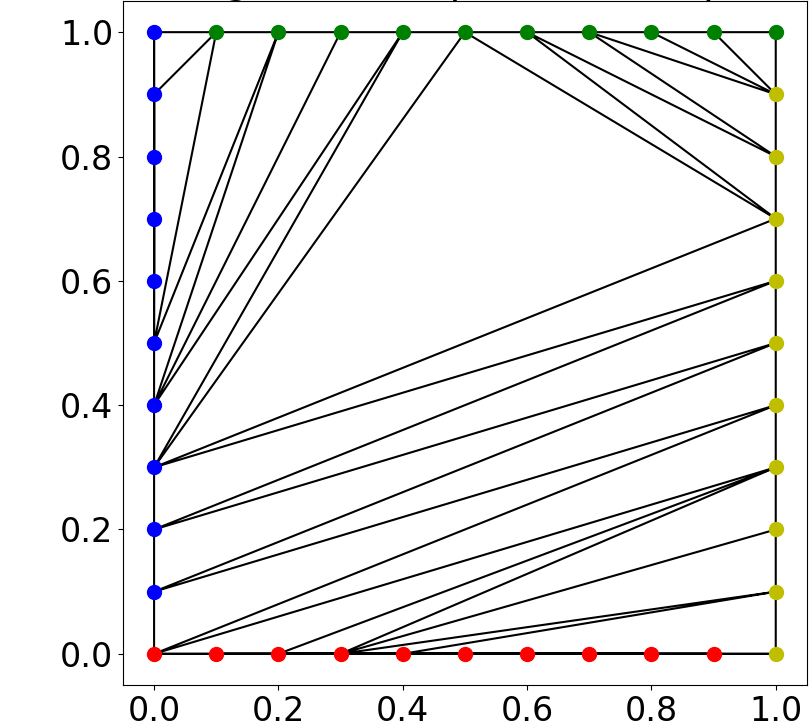
\includegraphics[width=0.9\textwidth, trim=37mm 14mm 6mm 6mm, clip]{images/fiber_creation/mesh_plots/out_0_1_0_tri.png}%
    %\caption{}%
    \label{fig:w_01}%
  \end{subfigure}
  \quad
  \begin{subfigure}[t]{0.31\textwidth}%
    \centering%
    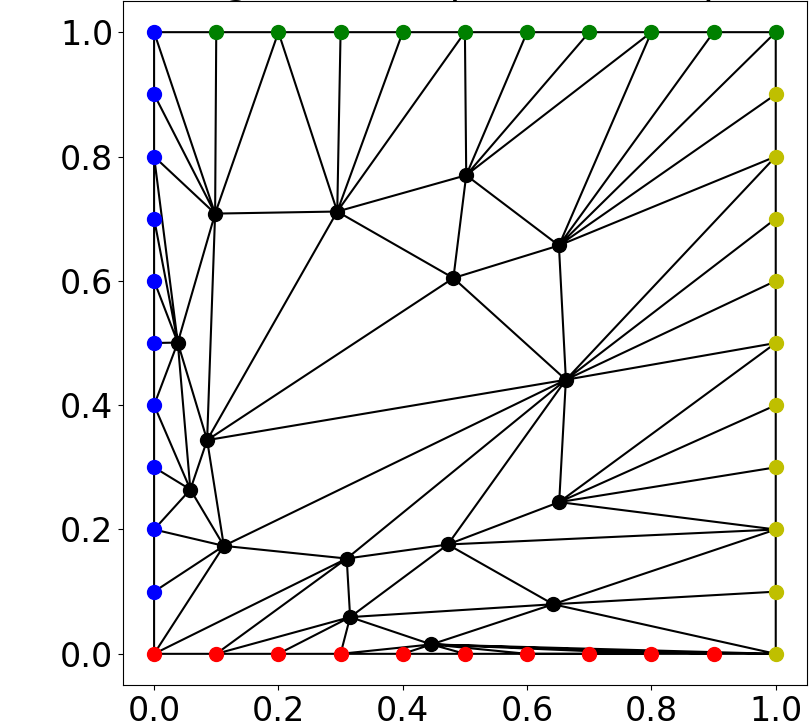
\includegraphics[width=0.9\textwidth, trim=37mm 14mm 6mm 6mm, clip]{images/fiber_creation/mesh_plots/out_1_1_0_tri.png}%
    %\caption{}%
    \label{fig:w_11}%
  \end{subfigure}
  \quad
  \begin{subfigure}[t]{0.31\textwidth}%
    \centering%
    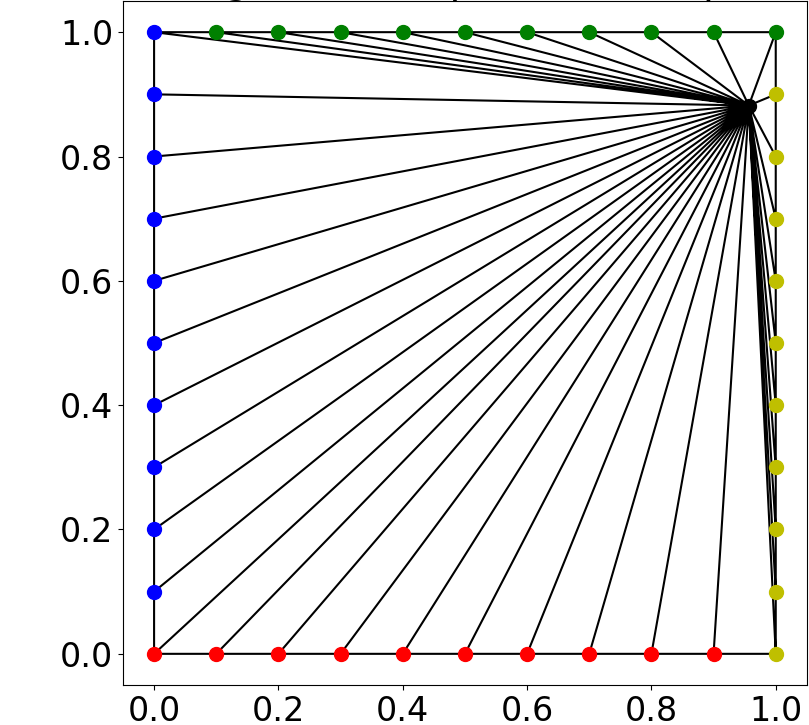
\includegraphics[width=0.9\textwidth, trim=37mm 14mm 6mm 6mm, clip]{images/fiber_creation/mesh_plots/out_2_1_0_tri.png}%
    %\caption{}%
    \label{fig:w_21}%
  \end{subfigure}\\
  
  % circle
  \begin{subfigure}[t]{0.31\textwidth}%
    \centering%
    \includegraphics[width=0.9\textwidth, trim=37mm 14mm 6mm 6mm, clip]{images/fiber_creation/mesh_plots/out_0_0_0_tri.png}% trim=left bottom right top, clip]
    %\caption{}%
    \label{fig:w_00}%
  \end{subfigure}
  \quad
  \begin{subfigure}[t]{0.31\textwidth}%
    \centering%
    \includegraphics[width=0.9\textwidth, trim=37mm 14mm 6mm 6mm, clip]{images/fiber_creation/mesh_plots/out_1_0_0_tri.png}%
    %\caption{}%
    \label{fig:w_10}%
  \end{subfigure}
  \quad
  \begin{subfigure}[t]{0.31\textwidth}%
    \centering%
    \includegraphics[width=0.9\textwidth, trim=37mm 14mm 6mm 6mm, clip]{images/fiber_creation/mesh_plots/out_2_0_0_tri.png}%
    %\caption{}%
    \label{fig:w_20}%
  \end{subfigure}
  
  \caption{Top row: Different triangulation methods for $S_M$, the color represents the solution $u$ of the harmonic map. Middle and bottom row: triangulation mapped to the parameter domain $\Omega_P$, for the unit square (middle) and the unit circle (bottom). Each column corresponds to one triangulation method.}%
  \label{fig:tri_triangulations}%
\end{figure}%



% ------------------
% resulting meshes
\begin{figure}%
  \centering%
  \hspace{0.24\textwidth}
  \begin{subfigure}[t]{0.24\textwidth}%
    \centering%
    \includegraphics[width=\textwidth]{images/fiber_creation/u_0.png}%
    \caption{First method}%
    \label{fig:tu_0}%
  \end{subfigure}
  \begin{subfigure}[t]{0.24\textwidth}%
    \centering%
    \includegraphics[width=\textwidth]{images/fiber_creation/u_1.png}%
    \caption{Second method}%
    \label{fig:tu_1}%
  \end{subfigure}
  \begin{subfigure}[t]{0.24\textwidth}%
    \centering%
    \includegraphics[width=\textwidth]{images/fiber_creation/u_2.png}%
    \caption{Third method}%
    \label{fig:tu_2}%
  \end{subfigure}\\
  
  % square
  \begin{subfigure}[t]{0.24\textwidth}%
    \centering%
    \includegraphics[width=\textwidth]{images/fiber_creation/quad_1.png}%
    \caption{Square, scheme 1}%
    \label{fig:tquad_1}%
  \end{subfigure}
  \begin{subfigure}[t]{0.24\textwidth}%
    \centering%
    \includegraphics[width=\textwidth, trim=26mm 14mm 6mm 6mm, clip]{images/fiber_creation/mesh_plots/out_0_1_0_w.png}%
    %\caption{}%
    \label{fig:tri_01}%
  \end{subfigure}
  \begin{subfigure}[t]{0.24\textwidth}%
    \centering%
    \includegraphics[width=\textwidth, trim=30mm 14mm 6mm 6mm, clip]{images/fiber_creation/mesh_plots/out_1_1_0_w.png}%
    %\caption{}%
    \label{fig:tri_11}%
  \end{subfigure}
  \begin{subfigure}[t]{0.24\textwidth}%
    \centering%
    \includegraphics[width=\textwidth, trim=30mm 14mm 6mm 6mm, clip]{images/fiber_creation/mesh_plots/out_2_1_0_w.png}%
    %\caption{}%
    \label{fig:tri_21}%
  \end{subfigure}\\[-4mm]
  
  % square adjusted
  \begin{subfigure}[t]{0.24\textwidth}%
    \centering%
    \includegraphics[width=\textwidth]{images/fiber_creation/quad_2.png}%
    \caption{Square, scheme 2}%
    \label{fig:tquad_2}%
  \end{subfigure}
  \begin{subfigure}[t]{0.24\textwidth}%
    \centering%
    \includegraphics[width=\textwidth, trim=26mm 14mm 6mm 6mm, clip]{images/fiber_creation/mesh_plots/out_0_2_0_w.png}%
    %\caption{}%
    \label{fig:tri_02}%
  \end{subfigure}
  \begin{subfigure}[t]{0.24\textwidth}%
    \centering%
    \includegraphics[width=\textwidth, trim=30mm 14mm 6mm 6mm, clip]{images/fiber_creation/mesh_plots/out_1_2_0_w.png}%
    %\caption{}%
    \label{fig:tri_12}%
  \end{subfigure}
  \begin{subfigure}[t]{0.24\textwidth}%
    \centering%
    \includegraphics[width=\textwidth, trim=30mm 14mm 6mm 6mm, clip]{images/fiber_creation/mesh_plots/out_2_2_0_w.png}%
    %\caption{}%
    \label{fig:tri_22}%
  \end{subfigure}\\[-4mm]
  
  % circle
  \begin{subfigure}[t]{0.24\textwidth}%
    \centering%
    \includegraphics[width=\textwidth]{images/fiber_creation/quad_0.png}%
    \caption{Circle, scheme 1}%
    \label{fig:tquad_0}%
  \end{subfigure}
  \begin{subfigure}[t]{0.24\textwidth}%
    \centering%
    \includegraphics[width=\textwidth, trim=26mm 14mm 6mm 6mm, clip]{images/fiber_creation/mesh_plots/out_0_0_0_w.png}% trim=left bottom right top, clip]
    %\caption{}%
    \label{fig:tri_00}%
  \end{subfigure}
  \begin{subfigure}[t]{0.24\textwidth}%
    \centering%
    \includegraphics[width=\textwidth, trim=26mm 14mm 6mm 6mm, clip]{images/fiber_creation/mesh_plots/out_1_0_0_w.png}%
    %\caption{}%
    \label{fig:tri_10}%
  \end{subfigure}
  \begin{subfigure}[t]{0.24\textwidth}%
    \centering%
    \includegraphics[width=\textwidth, trim=30mm 14mm 6mm 6mm, clip]{images/fiber_creation/mesh_plots/out_2_0_0_w.png}%
    %\caption{}%
    \label{fig:tri_20}%
  \end{subfigure}\\[-4mm]
  
  % circle adjusted
  \begin{subfigure}[t]{0.24\textwidth}%
    \centering%
    \includegraphics[width=\textwidth]{images/fiber_creation/quad_3.png}%
    \caption{Circle, scheme 2}%
    \label{fig:lquad_3}%
  \end{subfigure}
  \begin{subfigure}[t]{0.24\textwidth}%
    \centering%
    \includegraphics[width=\textwidth, trim=30mm 14mm 6mm 6mm, clip]{images/fiber_creation/mesh_plots/out_0_3_0_w.png}%
    %\caption{}%
    \label{fig:tri_03}%
  \end{subfigure}
  \begin{subfigure}[t]{0.24\textwidth}%
    \centering%
    \includegraphics[width=\textwidth, trim=30mm 14mm 6mm 6mm, clip]{images/fiber_creation/mesh_plots/out_1_3_0_w.png}%
    %\caption{}%
    \label{fig:tri_13}%
  \end{subfigure}
  \begin{subfigure}[t]{0.24\textwidth}%
    \centering%
    \includegraphics[width=\textwidth, trim=30mm 14mm 6mm 6mm, clip]{images/fiber_creation/mesh_plots/out_2_3_0_w.png}%
    %\caption{}%
    \label{fig:tri_23}%
  \end{subfigure}
  \caption{Meshes in $S_M$ for quadrangulations (rows) and triangulations (columns).}%
  \label{fig:tri_meshes}%
\end{figure}%


\section{Parallel Algorithm to Create Muscle and Fiber Meshes}\label{sec:parallel_algorithm}
parallel algorihm

\begin{algorithm}
  \begin{algorithmic}[1]%
    \Procedure{Create\_3D\_meshes\_parallel}{}
    \Require triangulated tubular surface
    \Ensure structured 3D volume mesh
    \Ensure 1D fiber meshes
    \Statex
    \State Solve Laplacian flow problem
    \State Trace streamlines in the gradient field
    \State Sample 1D fiber meshes
    \EndProcedure
  \end{algorithmic}%
  \caption{Parallel algorithm}%
  \label{alg:parallel_algorithm_1}%
\end{algorithm}%


\section{Results and Discussion}

conclusion for automatic segmentation: doesn't work for muscles, only for bones

If the quality of the images should be improved, it is also possible to manually edit the intermediate results of segmentations.

\section{Motor unit distribution}


\begin{equation*}
  \begin{array}{lll}
    p_\text{unscaled}(x) = \alpha^x, \quad \text{with }\alpha = 1.2\\[4mm]
    p(x) = \dfrac{p_\text{unscaled}(x) }{\ds\i{1}{n_\text{MU}} p_\text{unscaled}(x) \,\d x}\\[4mm]
    c(x) = \ds\i{1}{x}p(x)\,\d x\\[4mm]
    c^{-1}(x) 
    draw\_sample(): return round (c^{-1}(Y)), Y \sim N\big(c(0.5, n\text{MU}+0.5)\big) \text{ Zufallsvariable}
    p_\text{distance,unscaled}(\bff,(i,j)^\top,x) = \text{rbf} \vert \bfp_{\text{MU},x} - (i,j)^\top \vert * \bff
    p_\text{distance}(\bff,(i,j)^\top,x) = p_\text{distance,unscaled}(\bff,(i,j)^\top,x) / \ds\sum_{k=1}^{n_\text{MU}} p_\text{distance,unscaled}(\bff,(i,j)^\top,k)
    c_\text{distance}(\bff,(i,j)^\top,x) = \s{k=1}{x} p_\text{distance}(\bff,(i,j)^\top,k)
    \texttt{objective}(\bff) = \s{k=1,n_\text{MU}} a
  \end{array}
\end{equation*}



%  \chapter{An algorithm for mesh generation}
%    - introduction, need for fiber and 3d mesh
%    \section{State of the art}
%    - literature, laplace potential flow idea
%    \section{Data preprocessing}
%    - visual human dataset, methods to extract surface, approximation by spline surfaces
%    \section{Outline of the algorithm}
%    - pseudo code
%    \section{Plane mesh smoothing}
%    \section{Parallelization}
%    \section{Generation of fiber meshes}
%    - generation of muscle mesh, 3D and fibers, also in parallel
%  
% \chapter{Simulation scenarios}
%    \section{Simulation of electromyography with fiber-based formulation}
%      - scenario static-biceps-emg, composite meshes
%    \section{Simulation of electromyography with multidomain formulation}
%    \section{Muscle contraction with fiber-based formulation}
%      - fibers with contraction
%    \section{Muscle contraction with multidomain formulation}
% \chapter{Technical simulation results}
%    \section{Runtime evaluation}
%    - results and experiments, runtime, peak performance\\
%    - monodomain runtime comparison OpenCMISS opendihu
%    \section{parallel partitioning}
%    - parallel partitioning and weak scaling, opencmiss and opendihu 
%    \section{memory consumption}
%    - memory scaling OpenCMISS
% \chapter{biomechanical simulation results}
%    \section{Simulation of fatigue}
%    - monodomain, hh  shorten, fatigue effects
%    \section{Simulation of EMG}
%    - static biceps emg\\
%    - fibers with contraction\\
%    - multidomain with fat layer\\
%    - multidomain with contraction\\
%
%\part{Soft tissue robotics}
%\chapter{...}
%  - introduction, handling flexible objects, overview of different object types\\
%  - basics Lagrange formulation of cable\\
%  - cable with friction on surface\\
%  - placing cable\\
%  - peg-in-hole, with sparse grids\\
%  - simulation of 2d tissue\\
%  - gripping point estimation\\
%  
%  \cite{Maier2021}
%  
%\part{Conclusion}

% -------------- Literaturseite --------------------
\newpage

%\acsetup{pages/display=first,pages/name=true}

% Abbreviations
\printacronyms[include-classes=abbrev,name=Abbreviations]

% Nomenclature
\printacronyms[include-classes=nomencl,name=Nomenclature]


%\bibliography{references}{}
%\bibliographystyle{abbrv}
\printbibliography[%
  % change title
  title=Bibliography
]


% -------------- Anhang ------------
%\appendix
%\input{8_anhang.tex}

\end{document}

%\input{preambule/footer}
